\documentclass{article}
\usepackage{gensymb}
\usepackage[utf8]{inputenc}
\usepackage[spanish]{babel}
\usepackage{graphicx}
\usepackage{amsmath}
\usepackage{siunitx}
\usepackage{float}
\usepackage{booktabs}
\usepackage[top=1.9cm,bottom=3.67cm,left=1.9cm,right=1.32cm]{geometry}
\usepackage{fancyhdr}
\usepackage{lastpage}
\usepackage{subcaption}
\usepackage{amssymb}
\usepackage{amsmath}
\usepackage{cancel}

\pagestyle{fancy}
\fancyhf{}
\renewcommand{\headrulewidth}{0.4pt}
\renewcommand{\footrulewidth}{0.4pt}

\fancyhead[L]{UNCUYO -- Ing. Mecatrónica\\Mendoza -- Argentina}
\fancyhead[C]{AUTOMÁTICA Y MÁQUINAS ELÉCTRICAS\\ PROYECTO GLOBAL INTEGRADOR (Año 2024)}
\fancyhead[R]{Alumnos: Quiroga -- Armani\\17/02/2025}
\fancyfoot[C]{Página \thepage\ de \pageref{LastPage}}

\title{\textbf{PROYECTO GLOBAL\\INTEGRADOR:\\Control de Accionamiento de CA\\ con Motor Sincrónico de Imanes Permanentes}}
\author{
Armani, Matías\\
    \vspace{1cm}
Quiroga, Juan\\
    \textbf{Profesor:} \\
    Ing. Gabriel L. Julián
}
\date{Febrero 2025 \\ Universidad Nacional de Cuyo \\ Facultad de Ingeniería \\ Ingeniería Mecatrónica}

\begin{document}
\maketitle
\begin{abstract}
Este trabajo desarrolla un sistema de control automático para un accionamiento eléctrico basado en un motor síncrono de imanes permanentes (PMSM), aplicado al control de un brazo manipulador robótico de un grado de libertad. El proyecto integra modelado matemático, simulación dinámica y diseño de controladores, siguiendo los lineamientos establecidos para un sistema de lazo cerrado con control en cascada.

El análisis incluye un modelo dinámico no lineal del sistema físico, que abarca los subsistemas mecánico, electromagnético y térmico. Se diseñaron estrategias de control vectorial con desacoplamiento de torque y flujo magnético, utilizando un controlador PID optimizado para garantizar precisión en el seguimiento de consignas de posición y velocidad.

Los resultados de simulaciones en MATLAB/Simulink muestran la estabilidad y el desempeño del sistema bajo diferentes condiciones de operación y perturbaciones. Las conclusiones destacan la eficacia del diseño para aplicaciones didácticas y posibles mejoras en robustez térmica y precisión dinámica.
\end{abstract}



\newpage
\tableofcontents



\newpage
\section{Introducción}
En el presente trabajo se desarrolla un sistema de control automático para la posición y velocidad de un brazo manipulador robótico elemental (péndulo rígido actuado) de un solo grado de libertad, eje de rotación horizontal fijo a una base en el sistema de referencia inercial, con parámetros equivalentes variables según sea la carga útil transportada en el extremo. Dicho accionamiento va a realizarse con una máquina eléctrica de corriente alterna trifásica sincrónica con excitación por imanes permanentes, un inversor trifásico, un reductor de velocidad planetario, un sensor de posición en el eje mecánico del motor, tres sensores de corriente instantánea en la salida del inversor y un sensor de temperatura en los bobinados del estator.

En la primera parte del trabajo, se desarrollan modelos matemáticos adecuados para describir el comportamiento de los distintos subsistemas que componen al sistema global (mecánico, electromagnético y térmico); para describir el comportamiento del sistema y realizar una simulación dinámica a lazo abierto. Se analiza el modelo equivalente lineal invariante en el tiempo (LTI) y el modelo equivalente lineal de parámetros variables (LPV). Además, se realiza un análisis de estabilidad, controlabilidad y observabilidad.

En la segunda parte del trabajo, se diseñará, analizará y simulará un sistema de control de movimiento PID en cascada con modulador de torque equivalente, que incluye a su vez un observador de estado parcial, con el fin de manipular el brazo robótico para realizar las operaciones que se le solicite en forma óptima y precisa, verificando que los valores de trabajo se encuentren dentro de los valores permitidos mediante la realización de una simulación.



\section{Modelado, Análisis y Simulación dinámica del sistema físico a "Lazo Abierto"}

\textbf{Carga mecánica.}
La carga mecánica consiste en la articulación de un brazo manipulador robótico elemental (péndulo rígido actuado) con un solo grado de libertad (1 g.d.l.), eje de rotación horizontal fijo a una base en el sistema de referencia inercial; sometido a la acción externa de la aceleración de gravedad \( g \) (perturbación externa vertical constante), esquematizado en la Figura~\ref{fig:brazo_robotico}; con parámetros equivalentes variables según sea la carga útil transportada en el extremo (ver Ec.~\ref{eq:carga_mecanica}). La ecuación que describe el sistema es:

\begin{equation}
    J_l \frac{d\omega_l}{dt} = T_q - b_l \omega_l - T_l(t); \quad T_l(t) = g \cdot k_l \cdot \sin(\theta_l(t)) + T_{ld}(t),
    \label{eq:carga_mecanica}
\end{equation}
donde:
\begin{itemize}
    \item \( J_l \): Momento de inercia total (a eje de rotación).
    \item \( \omega_l \): Velocidad angular de la articulación del brazo robótico.
    \item \( T_q \): Torque impulsor (salida del tren de transmisión).
    \item \( b_l \): Coeficiente de fricción viscosa en la articulación.
    \item \( T_l(t) \): Torque de carga.
    \item \( g \): Aceleración gravitatoria.
    \item \( k_l \): Coeficiente \( k_l = m \cdot l_{cm} + m_l \cdot l_l \) en Torque de carga \( T_l \).
    \item \( \theta_l(t) \): Posición angular del eje de la carga.
    \item \( T_{ld}(t) \): Torque de perturbación por contacto.
\end{itemize}

Además, la posición angular \( \theta_l(t) \) del eje mecánico está relacionada con la velocidad angular mediante:
\begin{equation}
    \frac{d\theta_l(t)}{dt} = \omega_l(t) \iff \theta_l(t) = \int_{0}^{t} \omega_l(\xi) d\xi + \theta_l(0).
\end{equation}

\begin{figure}[H]
    \centering
    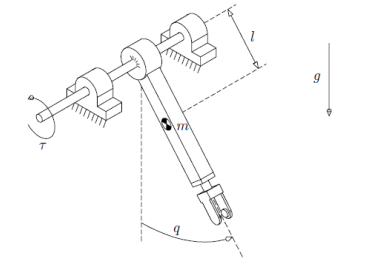
\includegraphics[width=0.5\textwidth]{Imagenes/brazo_robotico.png}
    \caption{Representación del brazo manipulador robótico.}
    \label{fig:brazo_robotico}
\end{figure}


\textbf{Tren de transmisión.}
Se considera una caja reductora reversible con sistema de engranajes planetarios (Figura~\ref{fig:tren_transmision}), asumiendo acoplamiento rígido
(sin elasticidad torsional y sin juego, holgura o “backlash”); momento de inercia equivalente y pérdidas de energía por fricción
interna, reflejados al eje de entrada y considerados junto con el motor.

Al considerar acoplamiento rígido podemos realizar una simplificación o compactación del subsistema mecánico completo,
ya que no se tiene en cuenta la deformación elástica que se produce en los engranajes cuando se transmite el torque. Es decir,
que podemos considerar la carga mecánica y el motor eléctrico como una unidad, obteniendo así un subsistema mecánico
completo de un grado de libertad “1 g.d.l.”.

Asumiendo un acoplamiento rígido, las relaciones entre las variables son:
\begin{equation}
\label{eq:transmision_velocidades}
    \omega_l(t) = \frac{1}{r} \omega_m(t),
\end{equation}
\begin{equation}
\label{eq:transmision_torques}
    T_q(t) = r T_d(t),
\end{equation}

donde:
\begin{itemize}
    \item \( r \): Relación de reducción del tren de transmisión.
    \item \( \omega_m(t) \): Velocidad angular del eje del motor.
    \item \( T_d(t) \): Torque de entrada al tren de transmisión.
    \item \( T_q(t) \): Torque de salida al tren de transmisión.
\end{itemize}

\textbf{Parámetro (constante):}
\begin{itemize}
    \item Relación de reducción total: \( r = 120.0 : 1 \).
\end{itemize}

\textbf{Especificaciones de operación (valores límite, no sobrepasar):}
\begin{itemize}
    \item Velocidad nominal (salida): \( n_{l,nom} = 60 \, \text{rpm} \) (\( \omega_{l,nom} = 6.28 \, \text{rad/s} \)).
    \item Torque nominal (salida): \( T_{q,nom} = 17.0 \, \text{N.m} \) (régimen continuo o rms).
    \item Torque pico (salida): \( T_{q,max} = 45.0 \, \text{N.m} \) (corta duración, aceleración).
\end{itemize}

\begin{figure}[H]
    \centering
    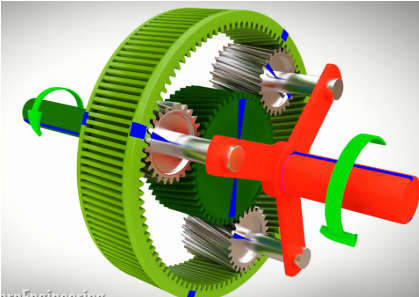
\includegraphics[width=0.5\textwidth]{Imagenes/tren_transmision.png}
    \caption{Representación del tren de transmisión planetario.}
    \label{fig:tren_transmision}
\end{figure}



\textbf{Máquina Eléctrica PMSM.}
Se considera una Máquina eléctrica de CA trifásica sincrónica con excitación por imanes permanentes (PMSM) y estator simétrico y equilibrado, con bornes de fases abc (coordenadas reales y “estacionarias”) conectados externamente en estrella (Y), con centro de estrella O (punto “neutro”) flotante (no accesible) y bornes de línea ABC accesibles desde el inversor electrónico trifásico.
El modelo matemático equivalente del subsistema mecánico del rotor de la máquina eléctrica (referido a Estator estacionario = fijo al sistema inercial de referencia) se describe mediante la ecuación:
\begin{equation}
    \label{eq:subsistema_mecanico_maquina_pmsm}
    J_m \frac{d\omega_m}{dt} = T_m - b_m \omega_m - T_d,
\end{equation}

\begin{equation}
    \frac{d\theta_m(t)}{dt} = \omega_m(t) \iff \theta_m(t) = \int_{0}^{t} \omega_m(\xi) d\xi + \theta_m(0).
\end{equation}

donde:
\begin{itemize}
    \item $J_m$: Momento de inercia (motor y caja).
    \item $\omega_m$: Velocidad angular del motor.
    \item $T_m$: Torque electromagnético generado por el motor.
    \item $b_m$: Coeficiente de fricción viscosa (motor y caja).
\end{itemize}


\subsection{Modelo matemático equivalente del subsistema mecánico completo}

Sustituyendo \( \omega_l(t) \) de (Ec.~\ref{eq:transmision_velocidades}) y \( T_q(t) \) de (Ec.~\ref{eq:transmision_torques}) en (Ec.~\ref{eq:carga_mecanica}):

\begin{equation}
    \frac{J_l}{r} \frac{d\omega_m(t)}{dt} = r T_d(t) - \frac{b_l}{r} \omega_m(t) - T_l(t),
\end{equation}

Despejando \( T_d(t) \) y reemplazando \( T_l(t) \) por su expresión equivalente:
\begin{equation}
\label{eq:expresion_Td_despejado}
    T_d(t) = \frac{J_l}{r^2} \frac{d\omega_m}{dt} + \frac{b_l}{r^2} \omega_m + \frac{1}{r} \left(g \cdot k_l \cdot \sin\left(\frac{\theta_m(t)}{r}\right) + T_{ld}(t)\right),
\end{equation}

y reemplazando \( T_d(t) \) de (Ec.~\ref{eq:expresion_Td_despejado}) en (Ec.~\ref{eq:subsistema_mecanico_maquina_pmsm}) se obtiene:
\begin{align}
    J_{\text{eq}} \frac{d\omega_m}{dt} &= -b_{\text{eq}} \omega_m + T_m - \frac{1}{r} \left(g \cdot k_l \cdot \sin\left(\frac{\theta_m(t)}{r}\right) + T_{ld}(t)\right), \\
    J_{\text{eq}} &= J_m + \frac{J_l}{r^2}, \\
    b_{\text{eq}} &= b_m + \frac{b_l}{r^2}, \\
    \theta_l(t) &= \frac{\theta_m(t)}{r}.
\end{align}

\textbf{Ecuaciones de estado.}
Las ecuaciones de estado del subsistema mecánico completo son:
\begin{equation}
\left\{
\begin{aligned}
    \dot{\theta}_m(t) &= \omega_m(t), \\
    \dot{\omega}_m(t) &= -\frac{b_{\text{eq}}}{J_{\text{eq}}} \omega_m(t) - \frac{g \cdot k_l}{J_{\text{eq}} r} \cdot \sin\left(\frac{\theta_m(t)}{r}\right) + \frac{1}{J_{\text{eq}}} T_m(t) - \frac{1}{J_{\text{eq}} r} T_{ld}(t), \\
    y(t) &= \theta_m(t).
\end{aligned}
\right.
\end{equation}

\textbf{Forma matricial.}
La representación del subsistema mecánico completo en espacio de estados es:


\begin{equation}
\left\{
\begin{aligned}
\begin{bmatrix}
    \dot{\theta}_m(t) \\
    \dot{\omega}_m(t)
\end{bmatrix}
&=
\underbrace{
\begin{bmatrix}
    \omega_m(t) \\
    -\frac{g \cdot k_l}{J_{\text{eq}} r} \cdot \sin\left(\frac{\theta_m(t)}{r}\right) -\frac{b_{\text{eq}}}{J_{\text{eq}}} \cdot \omega_m(t) 
\end{bmatrix}
}_{f(\theta_m(t),\omega_m(t))}
+
\begin{bmatrix}
    0 & 0 \\
    \frac{1}{J_{\text{eq}}} & -\frac{1}{J_{\text{eq}} r}
\end{bmatrix}
\begin{bmatrix}
    T_m(t) \\
    T_{ld}(t)
\end{bmatrix}, \\
y(t) &=
\begin{bmatrix}
    1 & 0
\end{bmatrix}
\begin{bmatrix}
    \theta_m(t) \\
    \omega_m(t)
\end{bmatrix}.
\end{aligned}
\right.
\end{equation}

Como se observa en (Ec. 14), este subsistema mecánico presenta una No Linealidad en el término senoidal de la expresión de la derivada de la segunda variable de estado, esto impide armar la matriz de estado A. En lugar de la matriz A, se tiene un campo vectorial No Lineal que relaciona las derivadas de las variables de estado con sus primitivas.

\begin{figure}[H]
    \centering
    % Subfigura (a) - Diagrama de bloques desagregado
    \begin{subfigure}[t]{\textwidth}
        \centering
        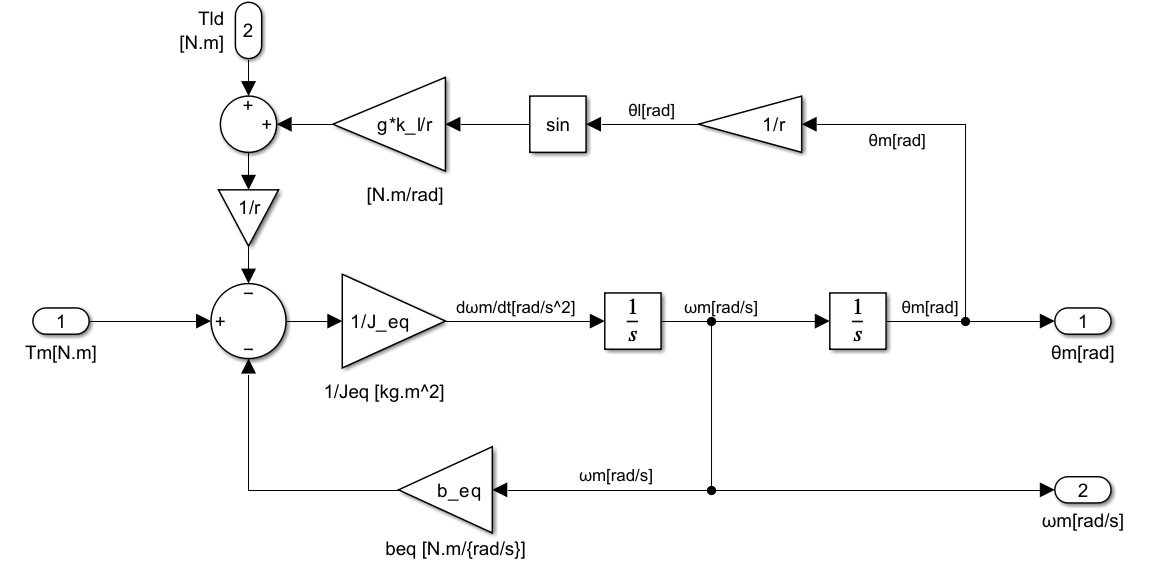
\includegraphics[width=0.75\textwidth]{Imagenes/bloque_subsistema_mecanico.png}
        \caption{Diagrama de bloques desagregado del subsistema mecánico completo.}
        \label{fig:diagrama_bloques_actualizado}
    \end{subfigure}
    
    \vspace{0.5cm} % Espacio entre subfiguras
    
    % Subfigura (b) - Bloque compacto
    \begin{subfigure}[t]{\textwidth}
        \centering
        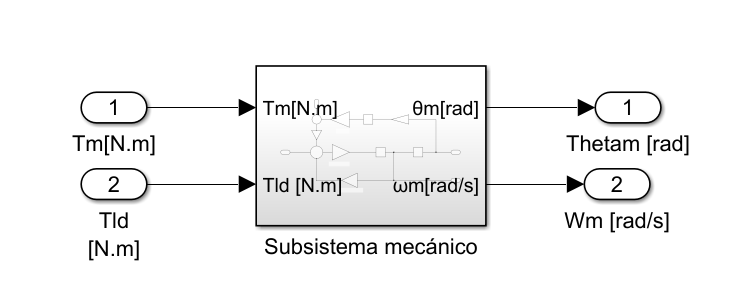
\includegraphics[width=0.5\textwidth]{Imagenes/bloque_subsistema_mecanico_compacto.png}
        \caption{Bloque compacto del subsistema mecánico.}
        \label{fig:bloque_subsistema_mecanico_compacto}
    \end{subfigure}
    
    \caption{Comparación entre el diagrama desagregado y el bloque compacto del subsistema mecánico.}
    \label{fig:subsistema_mecanico_comparacion}
\end{figure}


\subsection{Modelo dinámico del sistema físico completo}

El modelo dinámico del sistema físico completo considera la integración de los subsistemas mecánico, electromagnético y térmico de la máquina eléctrica. En esta sección se presenta el desarrollo del modelo global no lineal (NL), el modelo linealizado con parámetros variables (LPV) y el modelo simplificado lineal invariante (LTI).

\subsubsection{Modelo global no lineal (NL)}

Obtendremos el modelo no lineal (NL), para ``\(i_{ds}^r(t) \neq 0\)'' (caso general). Se obtendrán las ecuaciones vectoriales NL de estado y de salida (con estado inicial genérico, en coordenadas virtuales qd0) y luego se realizará el diagrama de bloques de estado (forma desagregada o escalar) incorporando las Transformaciones de Park virtuales.


\textbf{Subsistema electromagnético}

La velocidad del campo magnético rodante, llamada velocidad de sincronismo, debido a que es un motor síncrono, es igual a la velocidad angular del rotor $\omega_m$. Esta velocidad depende de la cantidad de pares de polos magnéticos y de las frecuencias de las señales eléctricas aplicadas en el estator $\omega_r$, a través de la siguiente relación:

\begin{equation}
    \frac{d\theta_r(t)}{dt} \equiv \omega_r(t) \iff \theta_r(t) = \int_{0}^{t} \omega_r(\xi) \, d\xi + \theta_r(0)
\end{equation}

\begin{equation}
    \theta_r(t) \equiv P_p \cdot \theta_m(t) \therefore \omega_r(t) = P_p \cdot \omega_m(t)
\end{equation}

El subsistema electromagnético del motor PMSM utiliza las transformaciones de Park para simplificar el análisis de variables trifásicas en coordenadas estacionarias, convirtiéndolas en un sistema de referencia rotativo que facilita el control y modelado del sistema.

\textbf{Transformación de Park Directa}

La transformación de Park directa convierte las coordenadas trifásicas de fase del estator (\(abc\)) en coordenadas \((qd0)\) que están fijadas al rotor y son virtuales. Esto permite expresar las variables en un marco rotativo, eliminando componentes oscilatorias en régimen estacionario. La matriz de transformación se expresa como:

\[
\begin{bmatrix}
    f_{qs}^r(t) \\
    f_{ds}^r(t) \\
    f_{0s}^r(t)
\end{bmatrix}
=
\frac{2}{3}
\begin{bmatrix}
    \cos(\theta_r(t)) & \cos\left(\theta_r(t) - \frac{2\pi}{3}\right) & \cos\left(\theta_r(t) + \frac{2\pi}{3}\right) \\
    \sin(\theta_r(t)) & \sin\left(\theta_r(t) - \frac{2\pi}{3}\right) & \sin\left(\theta_r(t) + \frac{2\pi}{3}\right) \\
    \frac{1}{2} & \frac{1}{2} & \frac{1}{2}
\end{bmatrix}
\begin{bmatrix}
    f_{as}(t) \\
    f_{bs}(t) \\
    f_{cs}(t)
\end{bmatrix}.
\]


\begin{figure}[H]
    \centering
    % Subfigura (a) - Diagrama de bloques desagregado
    \begin{subfigure}[t]{\textwidth}
        \centering
        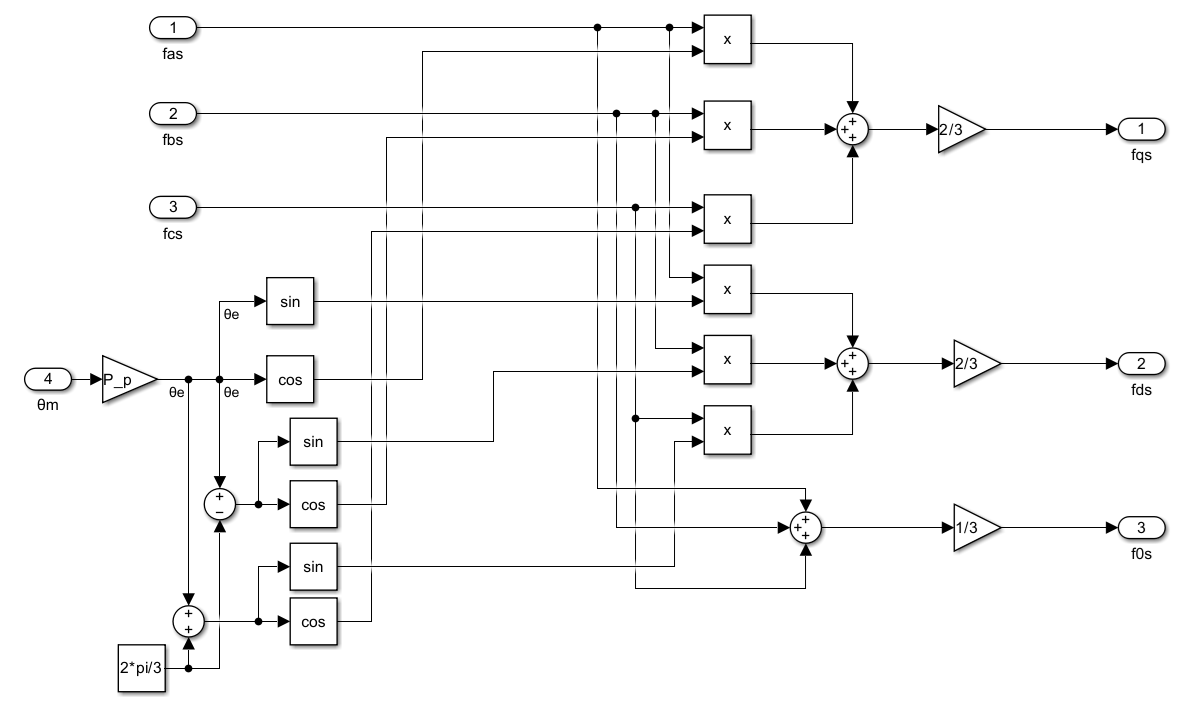
\includegraphics[width=0.85\textwidth]{Imagenes/ParkDirecta.png}
        \caption{Diagrama de bloques de la transformación directa de Park.}
        \label{fig:bloques_park_directa_desagregado}
    \end{subfigure}
    
    \vspace{0.5cm} % Espacio entre subfiguras
    
    % Subfigura (b) - Bloque compacto
    \begin{subfigure}[t]{\textwidth}
        \centering
        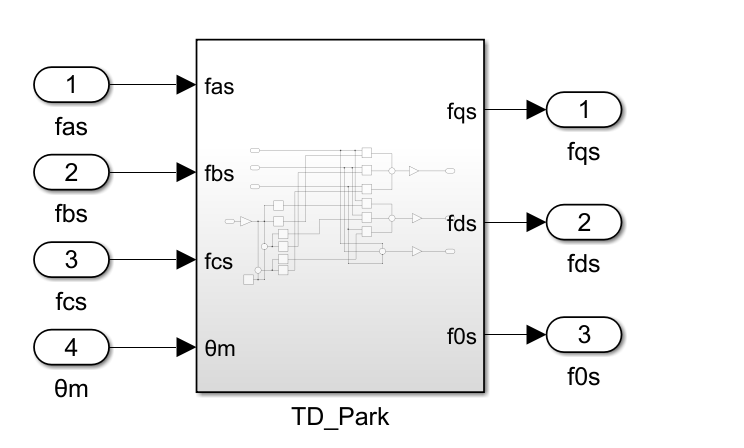
\includegraphics[width=0.45\textwidth]{Imagenes/CompactoParkDirecta.png}
        \caption{Bloque compacto de la transformación directa de Park.}
        \label{fig:bloque_park_directa_compacto}
    \end{subfigure}
    
    \caption{Comparación entre el diagrama desagregado y el bloque compacto de la transformada directa de Park.}
    \label{fig:bloques_park_directa}
\end{figure}

\textbf{Transformación de Park Inversa}

La transformación de Park inversa convierte las coordenadas \((qd0)\) de vuelta al sistema trifásico (\(abc\)), lo cual es útil para reconstruir las señales en el dominio original. La matriz inversa se define como:

\[
\begin{bmatrix}
    f_{as}(t) \\
    f_{bs}(t) \\
    f_{cs}(t)
\end{bmatrix}
=
\begin{bmatrix}
    \cos(\theta_r(t)) & \sin(\theta_r(t)) & 1 \\
    \cos\left(\theta_r(t) - \frac{2\pi}{3}\right) & \sin\left(\theta_r(t) - \frac{2\pi}{3}\right) & 1 \\
    \cos\left(\theta_r(t) + \frac{2\pi}{3}\right) & \sin\left(\theta_r(t) + \frac{2\pi}{3}\right) & 1
\end{bmatrix}
\begin{bmatrix}
    f_{qs}^r(t) \\
    f_{ds}^r(t) \\
    f_{0s}^r(t)
\end{bmatrix}.
\]


\begin{figure}[H]
    \centering
    % Subfigura (a) - Diagrama de bloques desagregado
    \begin{subfigure}[t]{\textwidth}
        \centering
        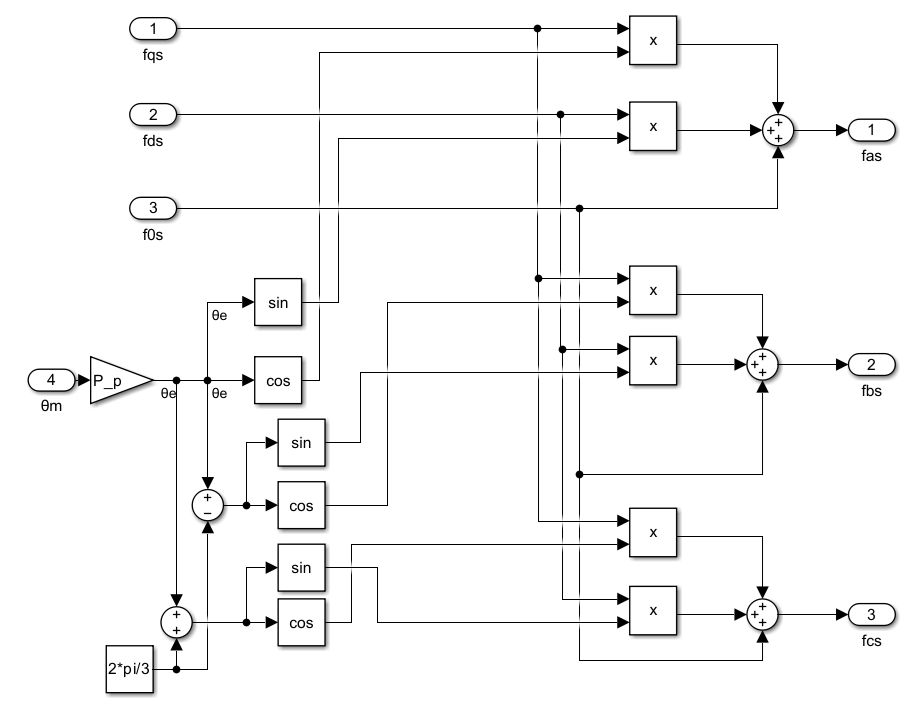
\includegraphics[width=0.80\textwidth]{Imagenes/ParkInversa.png}
        \caption{Diagrama de bloques de la transformación inversa de Park.}
        \label{fig:bloques_park_inversa_desagregado}
    \end{subfigure}
    
    \vspace{0.5cm} % Espacio entre subfiguras
    
    % Subfigura (b) - Bloque compacto
    \begin{subfigure}[t]{\textwidth}
        \centering
        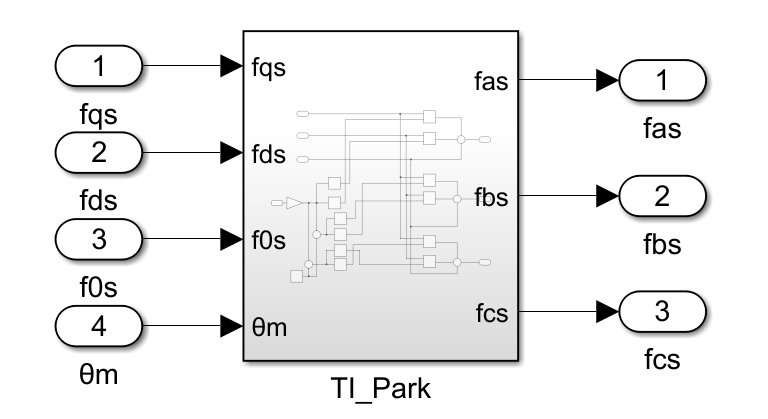
\includegraphics[width=0.4\textwidth]{Imagenes/CompactoParkInversa.png}
        \caption{Bloque compacto de la transformación inversa de Park.}
        \label{fig:bloque_park_inversa_compacto}
    \end{subfigure}
    
    \caption{Comparación entre el diagrama desagregado y el bloque compacto de la transformada inversa de Park.}
    \label{fig:bloques_park_inversa}
\end{figure}


Las transformaciones de coordenadas, tales como la transformada de Clark y la transformada de Park, se utilizan comúnmente en control de campo orientado de máquinas de CA trifásicas. La transformada de Clarke convierte las componentes del dominio del tiempo de un sistema trifásico (de un marco abc) a dos componentes de un marco estacionario ortogonal (\(\alpha \beta\)). La transformada de Park convierte las dos componentes del marco \(\alpha \beta\) a un marco de referencia giratorio ortogonal (dq). Implementar estas dos transformaciones de manera consecutiva simplifica los cálculos, ya que se convierte la forma de onda de corriente y tensión de CA en señales de CC.

\begin{figure}[H]
    \centering
    \begin{subfigure}[b]{0.45\textwidth}
        \centering
        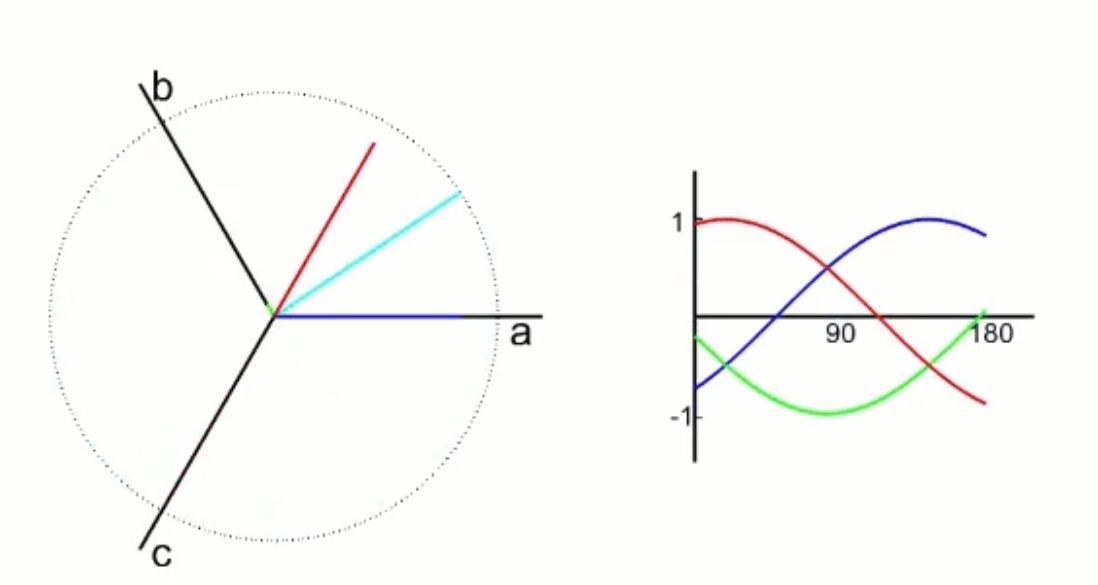
\includegraphics[width=\textwidth]{Imagenes/SistTrifasico(marcoABC).png}
        \caption{Componentes del dominio del tiempo de un sistema trifásico (de un marco abc).}
        \label{fig:componentes_marco_abc}
    \end{subfigure}
    \hfill
    \begin{subfigure}[b]{0.45\textwidth}
        \centering
        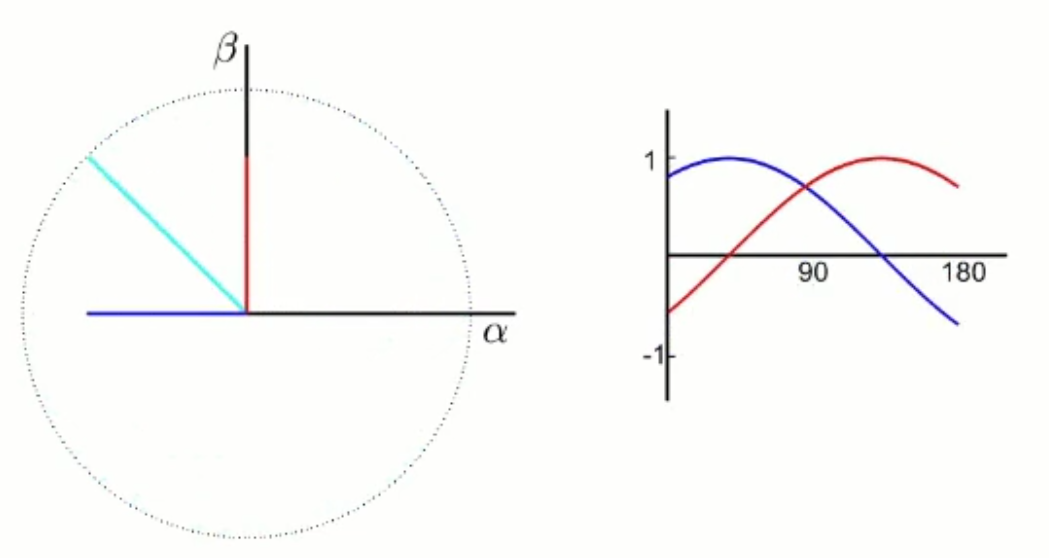
\includegraphics[width=\textwidth]{Imagenes/TransformadaClark.png}
        \caption{Señales resultantes de la transformación de Clarke (\(\alpha \beta\)).}
        \label{fig:transformacion_clark}
    \end{subfigure}
    \vskip\baselineskip
    \begin{subfigure}[b]{0.6\textwidth}
        \centering
        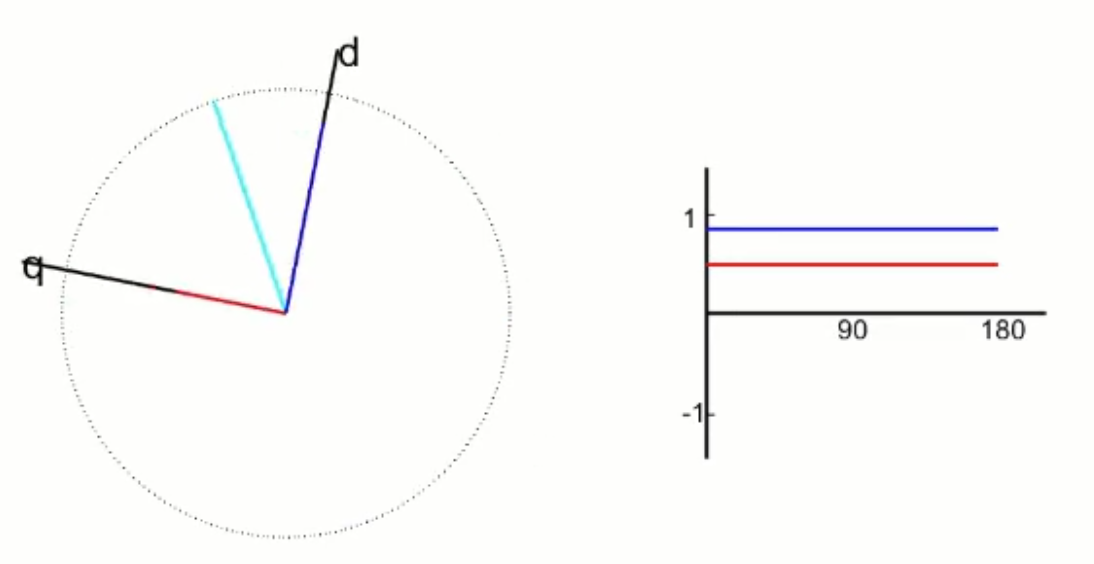
\includegraphics[width=\textwidth]{Imagenes/TransformadaPark.png}
        \caption{Señales resultantes de la transformación de Park (dq).}
        \label{fig:transformacion_park}
    \end{subfigure}
    \caption{Diagramas relacionados con las transformaciones de Clarke y Park.}
    \label{fig:transformaciones_clarke_park}
\end{figure}



\textbf{Modelo del subsistema electromagnético}

A continuación, se plantean las ecuaciones del balance de tensiones eléctricas equivalentes de estator referidas a coordenadas \(qd0^r\), incluyendo la expresión del torque electromagnético:


\begin{equation}
\left\{
\begin{aligned}
    v_{qs}^r(t) &= R_s(t) i_{qs}^r(t) + L_q \frac{d i_{qs}^r(t)}{dt} + \big(\lambda_m' + L_d i_{ds}^r(t)\big) \omega_r(t), \\
    v_{ds}^r(t) &= R_s(t) i_{ds}^r(t) + L_d \frac{d i_{ds}^r(t)}{dt} - L_q i_{qs}^r(t) \omega_r(t), \\
    v_{0s}^r(t) &= R_s(t) i_{0s}^r(t) + L_{ls} \frac{d i_{0s}^r(t)}{dt}, \\
    T_m(t) &= \frac{3}{2} P_p \lambda_m' i_{qs}^r(t) + \frac{3}{2} P_p (L_d - L_q) i_{ds}^r(t) i_{qs}^r(t).
\end{aligned}
\right.
\label{eq:SubsistemaElectromagnetico}
\end{equation}

Resolviendo el sistema anterior, se obtienen las expresiones para las derivadas de las corrientes en coordenadas \(qd0\):

\begin{equation}
\left\{
\begin{aligned}
    \frac{d i_{qs}^r(t)}{dt} &= \frac{1}{L_q} \Big( v_{qs}^r(t) - R_s(t) i_{qs}^r(t) - \big(\lambda_m' + L_d i_{ds}^r(t)\big) \omega_r(t) \Big), \\
    \frac{d i_{ds}^r(t)}{dt} &= \frac{1}{L_d} \Big( v_{ds}^r(t) - R_s(t) i_{ds}^r(t) + L_q i_{qs}^r(t) \omega_r(t) \Big), \\
    \frac{d i_{0s}^r(t)}{dt} &= \frac{1}{L_{ls}} \Big( v_{0s}^r(t) - R_s(t) i_{0s}^r(t) \Big).
\end{aligned}
\right.
\end{equation}

\textbf{Variación de la resistencia de los bobinados con la temperatura}

La resistencia de los bobinados del estator varía con la temperatura del bobinado (\(T_s^\circ(t)\)) de acuerdo con la siguiente ecuación:

\begin{equation}
    R_s(T_s^\circ(t)) = R_{s, \text{REF}} \cdot \Big( 1 + \alpha_\text{cu} \cdot (T_s^\circ(t) - T_{s, \text{REF}}) \Big),
\end{equation}

donde:
\begin{itemize}
    \item \(R_{s, \text{REF}}\): Resistencia de referencia medida a la temperatura \(T_{s, \text{REF}}\).
    \item \(\alpha_\text{cu}\): Coeficiente de variación de resistencia con la temperatura (pendiente de la recta).
    \item \(T_s^\circ(t)\): Temperatura del bobinado en el instante \(t\).
    \item \(T_{s, \text{REF}}\): Temperatura de referencia del bobinado.
\end{itemize}

La relación muestra un comportamiento lineal de incremento de la resistencia con la temperatura. Este fenómeno es crítico para el modelado térmico del motor.


\textbf{Parámetros eléctricos}

Los valores que se presentan a continuación son valores nominales medidos, con una tolerancia de error de \(\pm 1\%\), salvo aclaración específica.

\begin{table}[H]
\centering
\label{tabla_parametros_electricos}
\begin{tabular}{|l|l|l|}
\hline
\textbf{Parámetro} & \textbf{Símbolo} & \textbf{Valor medido} \\ \hline
Resistencia del estator & $R_s$ & $1.02 \, \Omega$ \\ \hline
Inductancia eje directo & $L_d$ & $6.6 \, \text{mH}$ \\ \hline
Inductancia eje en cuadratura & $L_q$ & $5.8 \, \text{mH}$ \\ \hline
Inductancia de dispersión & $L_{ls}$ & $0.8 \, \text{mH}$ \\ \hline
Flujo magnético del estator & $\lambda_m'$ & $0.016 \, \text{Wb}$ \\ \hline
Número de pares de polos & $P_p$ & $3$ \\ \hline
\end{tabular}
\caption{Parámetros eléctricos del subsistema eléctrico}
\end{table}

\textbf{Especificaciones de operación eléctricas}

Las especificaciones presentadas corresponden a bornes de fases \(abc\) del estator y son valores límite que no se deben sobrepasar.

\begin{table}[H]
\centering
\label{tabla_especificaciones_electricas}
\begin{tabular}{|l|l|l|}
\hline
\textbf{Especificación} & \textbf{Símbolo} & \textbf{Valor límite} \\ \hline
Velocidad nominal del rotor & $\omega_m$ & $691.15 \, \text{rad/s}$ \\ \hline
Tensión nominal de línea & $V_{sl}$ & $30 \, \text{\(V_{CA RMS}\)}$ \\ \hline
Corriente nominal & $I_s$ & $0.4 \, \text{A RMS}$ \\ \hline
Corriente máxima & $I_{s, \text{max}}$ & $2.0 \, \text{A RMS}$ \\ \hline
\end{tabular}
\caption{Especificaciones de operación del subsistema eléctrico}
\label{tabla:especificaciones_operacion_electricas}
\end{table}

\begin{figure}[H]
    \centering
    % Subfigura (a) - Diagrama de bloques desagregado
    \begin{subfigure}[t]{\textwidth}
        \centering
        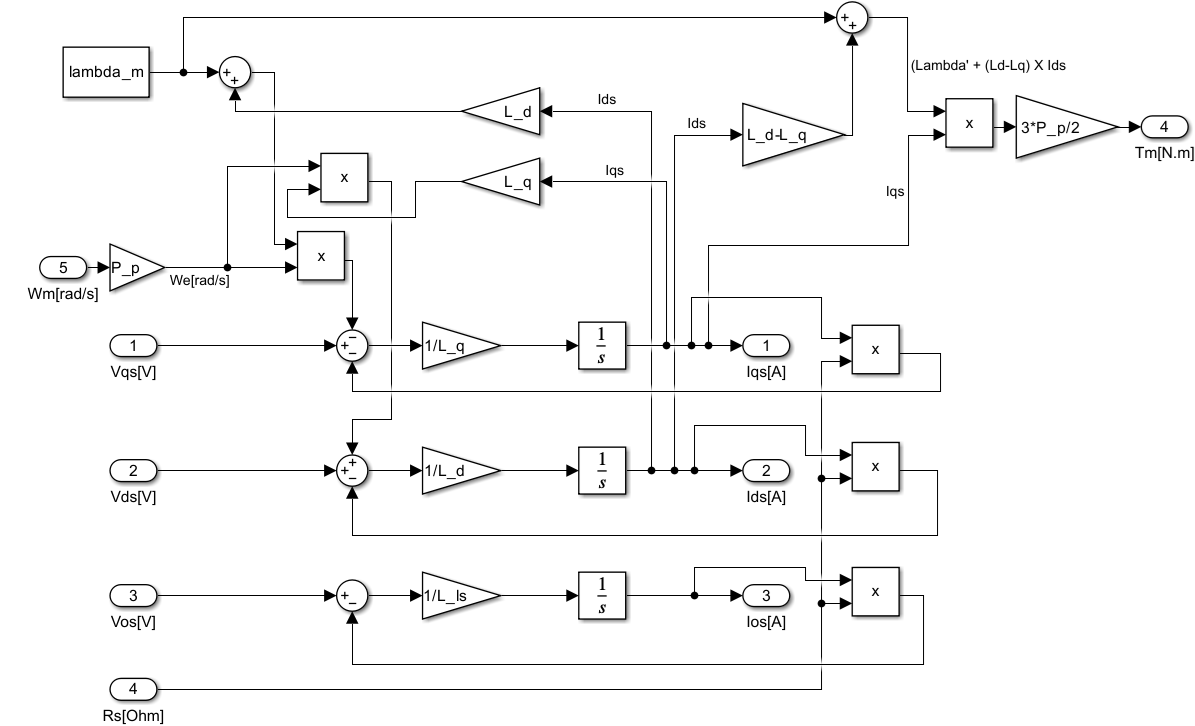
\includegraphics[width=0.90\textwidth]{Imagenes/BloquesSistElectromagnetico.png}
        \caption{Diagrama de bloques desagregado del subsistema electromagnético.}
        \label{fig:BloquesElectromagnetico}
    \end{subfigure}
    
    \vspace{0.5cm} % Espacio entre subfiguras
    
    % Subfigura (b) - Bloque compacto
    \begin{subfigure}[t]{\textwidth}
        \centering
        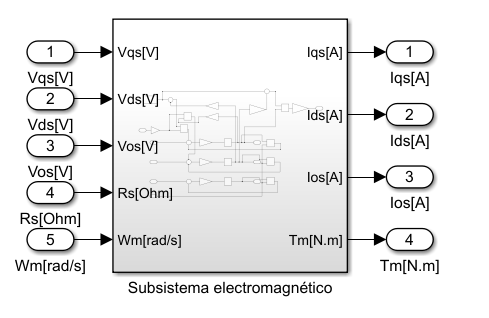
\includegraphics[width=0.4\textwidth]{Imagenes/CompactoSistElectromagnetico.png}
        \caption{Bloque compacto del subsistema electromagnético.}
        \label{fig:bloque_electromagnetico_compacto}
    \end{subfigure}
    
    \caption{Comparación entre el diagrama desagregado y el bloque compacto del subsistema electromagnético.}
    \label{fig:bloques_park_inversa}
\end{figure}

\textbf{Subsistema térmico}

El subsistema térmico de la máquina eléctrica se modela mediante el balance energético en el estator, considerando las pérdidas resistivas y los intercambios de calor con el entorno. Este modelo permite evaluar las temperaturas en diferentes componentes de la máquina.

\textbf{Modelo del subsistema térmico}

El balance energético en el estator se expresa mediante la siguiente ecuación diferencial, donde \( T_s(t) \) es la temperatura del estator en un instante \( t \):

\begin{equation}
\frac{dT_s(t)}{dt} = \frac{1}{C_{ts}} \cdot \Big( P_{\text{perd}}(t) - \frac{1}{R_{ts-\text{amb}}} \big( T_s(t) - T_{\text{amb}} \big) \Big)
\end{equation}


Potencia disipada real en coordenadas abc:

\begin{equation}
P_{\text{perd, abc}}(t) = R_s(t) \cdot \Big( i_{as}^2(t) + i_{bs}^2(t) + i_{cs}^2(t) \Big)
\end{equation}

Potencia equivalente virtual en coordenadas qd0:

\begin{equation}
P_{\text{perd, qd0}}(t) = \frac{3}{2} \cdot R_s(t) \cdot \Big( i_{qs}^r(t)^2 + i_{ds}^r(t)^2 + 2 \cdot i_{0s}^r(t)^2 \Big)
\end{equation}

Sustituyendo \( P_{\text{perd, qd0}}(t) \) en el balance térmico, obtenemos:

\begin{equation}
\label{eq:subsistema_termico}
\frac{dT_s(t)}{dt} = \frac{1}{C_{ts}} \Big[ \frac{3}{2} \cdot R_s(t) \cdot \Big( i_{qs}^r(t)^2 + i_{ds}^r(t)^2 + 2 \cdot i_{0s}^r(t)^2 \Big) - \frac{1}{R_{ts-\text{amb}}} \big( T_s(t) - T_{\text{amb}} \big) \Big]
\end{equation}

Esta es la expresión final que describe el modelo del subsistema térmico de la máquina eléctrica. Tal ecuación es fundamental para el análisis del comportamiento térmico bajo diferentes condiciones de operación.


\textbf{Parámetros térmicos}

Los parámetros utilizados en el modelo térmico tienen valores nominales medidos y se presentan con una tolerancia de error de \(\pm 1\%\).

\begin{table}[H]
\centering
\label{tabla_parametros_termicos}
\begin{tabular}{|l|l|l|}
\hline
\textbf{Parámetro} & \textbf{Símbolo} & \textbf{Valor medido} \\ \hline
Capacidad térmica del estator & $C_{ts}$ & $0.818 \, \text{Js/°C}$ \\ \hline
Resistencia térmica estator-ambiente & $R_{\text{ts-amb}}$ & $146.7 \, \text{°C/W}$ \\ \hline
Constante de tiempo térmica & $\tau_{\text{ts-amb}}$ & $120 \, \text{s}$ \\ \hline
\end{tabular}
\caption{Parámetros térmicos del subsistema térmico}
\end{table}

\textbf{Especificaciones de operación térmica}

Las siguientes especificaciones corresponden a valores límite del subsistema térmico que no se deben sobrepasar.

\begin{table}[H]
\centering
\label{tabla_especificaciones_termicas}
\begin{tabular}{|l|l|l|}
\hline
\textbf{Especificación} & \textbf{Símbolo} & \textbf{Valor límite} \\ \hline
Temperatura máxima del estator & $T_{s, \text{max}}$ & $115 \, \text{°C}$ \\ \hline
Rango de Temperatura Ambiente de Operación & $T^\circ_{amb}$ & $[-15,40]\,\text{°C}$ \\ \hline
\end{tabular}
\caption{Especificaciones de operación térmica del subsistema}
\end{table}

\begin{figure}[H]
    \centering
    % Subfigura (a) - Diagrama de bloques desagregado
    \begin{subfigure}[t]{\textwidth}
        \centering
        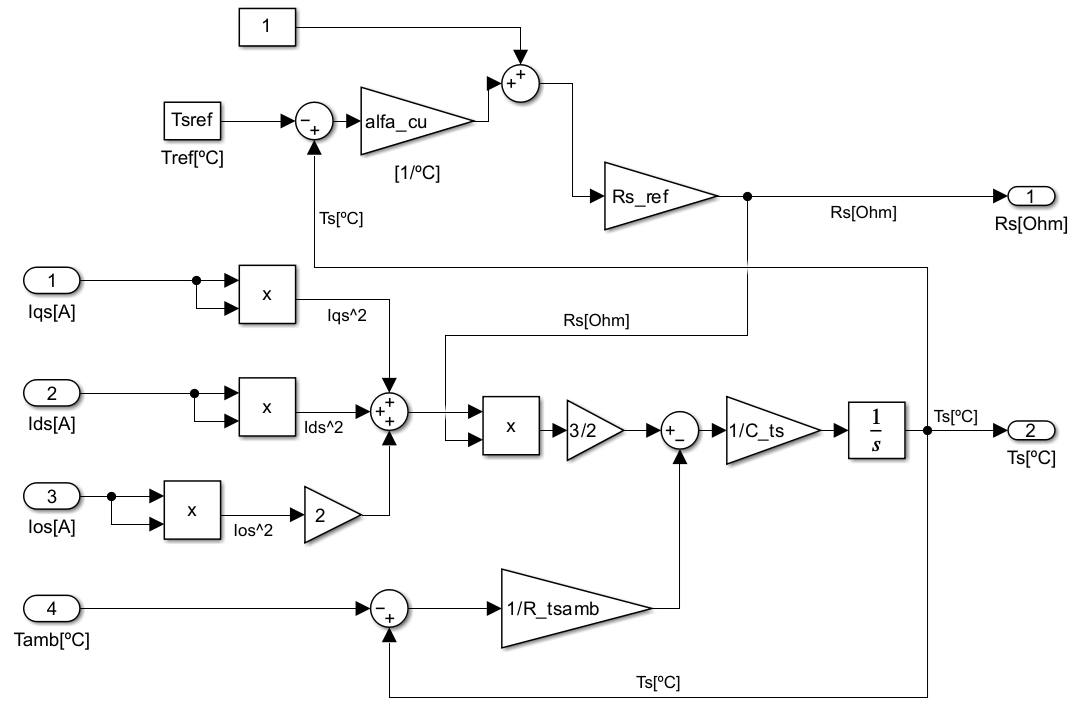
\includegraphics[width=0.85\textwidth]{Imagenes/BloquesSistTermico.png}
        \caption{Diagrama de bloques desagregado del subsistema térmico.}
        \label{fig:bloques_termico_desagregado}
    \end{subfigure}
    
    \vspace{0.5cm} % Espacio entre subfiguras
    
    % Subfigura (b) - Bloque compacto
    \begin{subfigure}[t]{\textwidth}
        \centering
        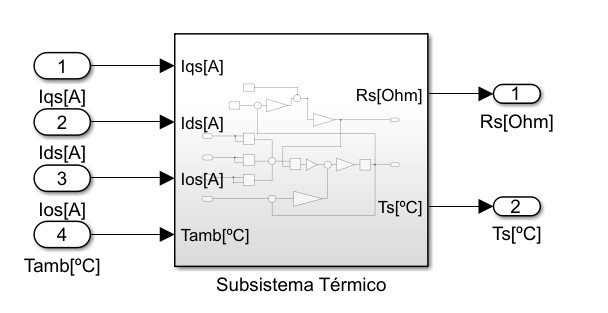
\includegraphics[width=0.4\textwidth]{Imagenes/CompactoSistTermico.png}
        \caption{Bloque compacto del subsistema térmico.}
        \label{fig:bloques_termico_compacto}
    \end{subfigure}
    
    \caption{Comparación entre el diagrama desagregado y el bloque compacto del subsistema térmico.}
    \label{fig:bloques_termico}
\end{figure}

\textbf{Modelo Global No Lineal}

A partir de las ecuaciones obtenidas en las secciones anteriores, se integran en un sistema de ecuaciones diferenciales no lineales, donde las derivadas de las variables de estado están despejadas. Este modelo se presenta en forma desagregada escalar y en el espacio de estado matricial. La matriz \(\mathbf{A}\) en este caso no es cuadrada, ya que contiene los términos no lineales que relacionan las derivadas de las variables de estado con las mismas variables de estado no derivadas.

El sistema incluye:

\begin{itemize}
    \item Las ecuaciones de la posición angular \(\theta_m(t)\) y velocidad angular \(\omega_m(t)\) del eje mecánico del motor, donde \(T_m(t)\) es sustituido por su equivalente en función de \(i_{qs}^r(t)\) e \(i_{ds}^r(t)\).
    \item Las ecuaciones de las corrientes virtuales \(i_{qs}^r(t)\), \(i_{ds}^r(t)\) e \(i_{0s}^r(t)\), donde \(\omega_r(t)\) es sustituido por \(P_p \cdot \omega_m(t)\).
    \item La ecuación del balance térmico para la temperatura del estator \(T_s(t)\).
\end{itemize}

\textbf{Ecuaciones del sistema desagregado escalar}

\begin{equation}
\left\{
\begin{aligned}
    \dot{\theta}_m(t) &= \omega_m(t), \\
    \dot{\omega}_m(t) &= \frac{1}{J_{eq}} \Bigg[ \frac{3}{2} P_p \Big( \lambda_m' i_{qs}^r(t) + (L_d - L_q) i_{ds}^r(t) i_{qs}^r(t) \Big) - b_{eq} \omega_m(t) - g \cdot k_l \sin\Bigg(\frac{\theta_m(t)}{r}\Bigg) - \frac{1}{r} T_{ld}(t) \Bigg], \\
    \frac{d i_{qs}^r(t)}{dt} &= \frac{1}{L_q} \Big( v_{qs}^r(t) - R_s(t) i_{qs}^r(t) - (\lambda_m' + L_d i_{ds}^r(t)) P_p \cdot \omega_m(t) \Big), \\
    \frac{d i_{ds}^r(t)}{dt} &= \frac{1}{L_d} \Big( v_{ds}^r(t) - R_s(t) i_{ds}^r(t) + L_q i_{qs}^r(t) P_p \cdot \omega_m(t) \Big), \\
    \frac{d i_{0s}(t)}{dt} &= \frac{1}{L_{ls}} \Big( v_{0s}(t) - R_s(t) i_{0s}(t) \Big), \\
    \frac{d T_s(t)}{dt} &= \frac{1}{C_{ts}} \Bigg[ \frac{3}{2} R_s(t) \Big( (i_{qs}^r(t))^2 + (i_{ds}^r(t))^2 + 2 \cdot (i_{0s}(t))^2 \Big) - \frac{1}{R_{ts-amb}} \big( T_s(t) - T_{amb}(t) \big) \Bigg].
\end{aligned}
\right.
\end{equation}


Las variables de estado, las manipuladas y las de perturbación se definen como:

\[
\mathbf{x}(t) = 
\begin{bmatrix}
    \theta_m(t) \\
    \omega_m(t) \\
    i_{qs}^r(t) \\
    i_{ds}^r(t) \\
    i_{0s}(t) \\
    T_s(t)
\end{bmatrix}, \quad
\mathbf{u}(t) = 
\begin{bmatrix}
    v_{qs}^r(t) \\
    v_{ds}^r(t) \\
    v_{0s}(t)
\end{bmatrix}, \quad
\mathbf{d}(t) = 
\begin{bmatrix}
    T_{ld}(t) \\
    T_{amb}(t)
\end{bmatrix}.
\]

\noindent\textbf{Forma matricial.}
La representación del sistema global no lineal completo en el espacio de estados es:

\begin{equation}
\left\{
\begin{aligned}
\begin{bmatrix}
    \dot{\theta}_m(t) \\
    \dot{\omega}_m(t) \\
    \dot{i_{qs}^r}(t) \\
    \dot{i_{ds}^r}(t) \\
    \dot{i_{0s}^r}(t) \\
    \dot{T}_s(t)
\end{bmatrix}
&=
\underbrace{
\begin{bmatrix}
    \omega_m(t) \\
    \frac{1}{J_{eq}} \Bigg[ \frac{3}{2} P_p \Big( \lambda_m' i_{qs}^r(t) + (L_d - L_q) i_{ds}^r(t) i_{qs}^r(t) \Big) - b_{eq} \omega_m(t) - g \cdot k_l \sin\Bigg(\frac{\theta_m(t)}{r}\Bigg) \Bigg] \\
    \frac{1}{L_q} \Big(- R_s(t) i_{qs}^r(t) - (\lambda_m' + L_d i_{ds}^r(t)) P_p \cdot \omega_m(t) \Big) \\
    \frac{1}{L_d} \Big( - R_s(t) i_{ds}^r(t) + L_q i_{qs}^r(t) P_p \cdot \omega_m(t) \Big) \\
    \frac{1}{L_{0s}} \Big( - R_s(t) i_{0s}(t) \Big) \\
    \frac{1}{C_{ts}} \Bigg[ \frac{3}{2} R_s(t) \Big( (i_{qs}^r(t))^2 + (i_{ds}^r(t))^2 + 2 \cdot (i_{0s}(t))^2 \Big) - \frac{1}{R_{ts-amb}} T_s(t) \Bigg]
\end{bmatrix}
}_{f(\theta_m(t),\omega_m(t),i_{qs}^r(t),i_{ds}^r(t),i_{0s}^r(t),T^\circ_s(t))}
 \\ &+
\underbrace{
\begin{bmatrix}
0 & 0 & 0 \\
0 & 0 & 0 \\
\frac{1}{L_q} & 0 & 0 \\
0 & \frac{1}{L_d} & 0 \\
0 & 0 & \frac{1}{L_{\mathrm{ls}}} \\
0 & 0 & 0
\end{bmatrix} }_{B_c}
\, u(t)
+
\underbrace{\begin{bmatrix}
0 & 0 \\
\frac{1}{J_{\mathrm{eq}} r} & 0 \\
0 & 0 \\
0 & 0 \\
0 & 0 \\
0 & \frac{1}{C_{\mathrm{ts}} R_{\mathrm{ts},\mathrm{amb}}}
\end{bmatrix} }_{B_d}
\, d(t), \\
y(t) &=
\underbrace{\begin{bmatrix}
    1 & 0 & 0 & 0 & 0 & 0
\end{bmatrix}}_{C}
\, x(t).
\end{aligned}
\right.
\end{equation}

\begin{figure}[H]
    \centering
    % Subfigura (a) - Diagrama de bloques desagregado
    \begin{subfigure}[t]{\textwidth}
        \centering
        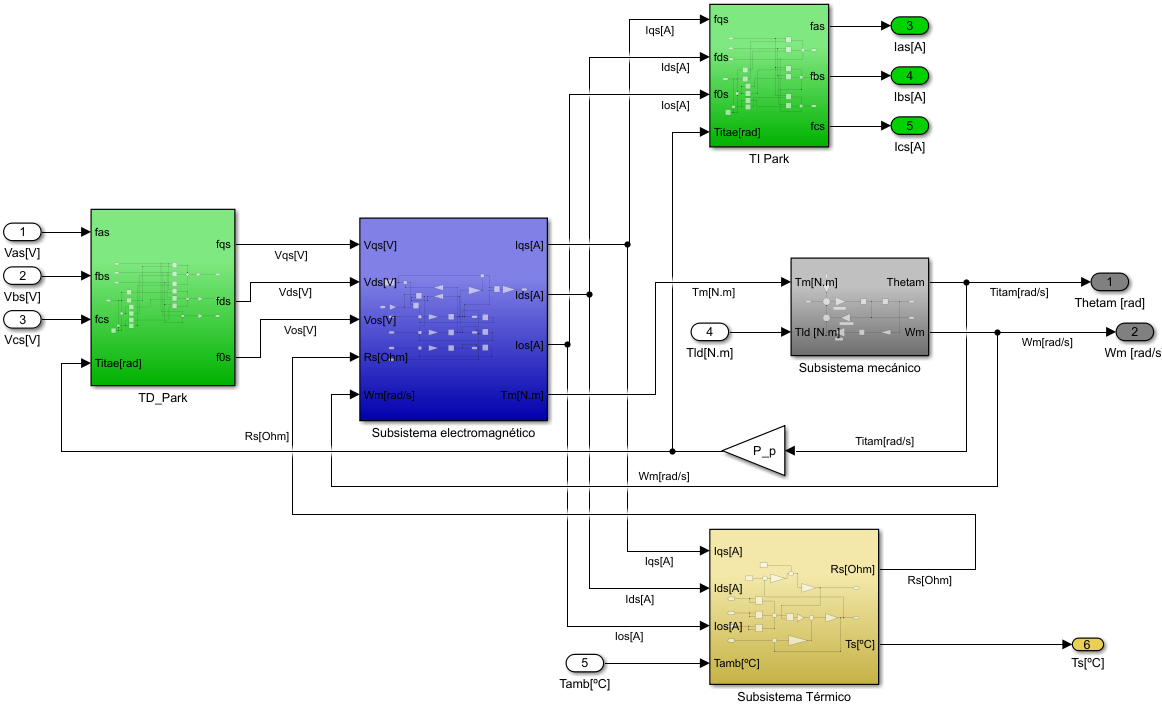
\includegraphics[width=0.9\textwidth]{Imagenes/Diagrama_Global_NoLineal.png}
        \caption{Diagrama de bloques desagregado del sistema global no lineal.}
        \label{fig:bloques_global_nolineal}
    \end{subfigure}
    
    \vspace{0.5cm} % Espacio entre subfiguras
    
    % Subfigura (b) - Bloque compacto
    \begin{subfigure}[t]{\textwidth}
        \centering
        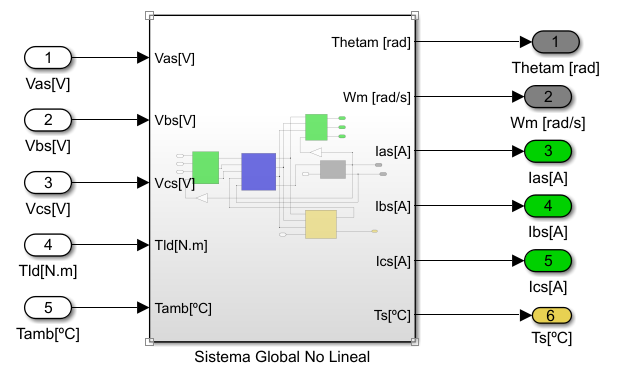
\includegraphics[width=0.45\textwidth]{Imagenes/CompactoGlobalNoLineal.png}
        \caption{Bloque compacto del sistema global no lineal.}
        \label{fig:modelo_global_nolineal}
    \end{subfigure}
    
    \caption{Comparación entre el diagrama desagregado y el bloque compacto del sistema global no lineal .}
    \label{fig:bloques_global}
\end{figure}



\subsubsection{Modelo global linealizado con parámetros variables (LPV)}

Para obtener el modelo global linealizado con parámetros variables (LPV), para ``\(i_{ds}^r(t) \neq 0\)'' (caso general), se parte del modelo Global No Lineal mediante aproximación con serie de Taylor truncada de 1° orden. El problema se divide en 2 partes, un espacio de operación global No Lineal (cuasi-estacionario) y un modelo dinámico LPV (pequeñas variaciones locales), que es función de parámetros variables según el punto de operación. El sistema dinámico no-lineal se puede representar como:

\begin{equation}
\label{eq:representacion_no_lineal_sistema_dinamico}
\left\{
\begin{aligned}
    \dot{x}(t) &= f(x(t),u(t)); && x(t_0) = x_0, \\ 
    y(t) &= C \cdot x(t) 
\end{aligned}
\right.
\end{equation}

Teniendo en cuenta que para una variable genérica: $z(t) = Z_0(t) + \Delta z(t)$ donde $Z_0(t)$ es el movimiento del sistema en el espacio de operación, los cuales son constates o cuasiestacionarios y $\Delta z(t)$ representa la dinámica local en cada punto de operación, teniendo una magnitud pequeña pero con variaciones rápidas en el tiempo. De esta manera, el sistema dinámico no-lineal anterior se transforma en:

\begin{equation}
\left\{
\begin{aligned}
\dot{x}(t) &= \dot{X_0}(t) + \Delta \dot{x}(t) = f(X_0(t) + \Delta x(t), U_0(t) + \Delta u(t)) \\
X_0(0) + \Delta x(0) &= x_0 & \Longrightarrow X_0(0) \equiv x_0, \Delta x(0) \equiv 0 \\
Y_0(t) + \Delta y(t) &= C(X_0(t) + \Delta x(t)) & \Longrightarrow Y_0(t) = CX_0(t); \Delta y(t) = C\Delta x(t)
\end{aligned}
\right.
\end{equation}

En los sistemas no lineales los puntos de equilibrio son todos aquellos en donde la variación de energía se ha disipado completamente (equilibrio dinámico). Es decir, los puntos de equilibrio son todos aquellos en donde las derivadas de las variables de estado son nulas.

\begin{equation*}
\text{Equilibrios:} \quad \dot{x}(t) = 0 = f(x(t),u(t))
\end{equation*}

A todos los pares valores de $x(t)$ e $u(t)$ que satisfacen la igualdad se lo denomina puntos de operación $(X_0,U_0)$. Los puntos de operación pueden ser constantes $\{X_0,U_0\}$ o presentar variaciones relativamente lentas en el tiempo (cuasi-estacionarios) $\{X_0(t),U_0(t)\}$.

Realizamos una expansión en serie de Taylor truncada a 1° orden (despreciando términos orden superior):
\begin{equation}
f(X_0(t) + \Delta x(t), U_0(t) + \Delta u(t)) \approx f(X_0(t),U_0(t)) + \left.\frac{\partial f}{\partial x}\right|_0 (t) \cdot \Delta x(t) + \left.\frac{\partial f}{\partial u}\right|_0 (t) \cdot \Delta u(t)
\end{equation}

Si sustituimos esta última expresión en la (Ec.~\ref{eq:representacion_no_lineal_sistema_dinamico}), vemos la división del problema en dos partes anteriormente mencionada:

1. Una parte no lineal, que representa el espacio de operación global NL (cuasi-estacionario):
  \begin{equation}
  \dot{X}_0(t) = f(X_0(t),U_0(t)) \approx 0/ete; \quad X_0(0) = x_0
  \label{Ec.25}
  \end{equation}

Que en nuestro sistema en particular esta formado por el siguiente sistema de ecuaciones:

\begin{equation}
\left\{
\begin{aligned}
\frac{d\theta_{mO}}{dt}(t) &= \omega_{mO}(t) = cte \\
\frac{d\omega_{mO}}{dt}(t) &= \frac{1}{J_{eq}}\left[-b_{eq}\omega_{mO}(t) + \frac{3}{2}P_p[\lambda_m' + (L_d - L_q)i^r_{dsO}(t)]i^r_{qsO}(t) - g \cdot k_l \sin\Bigg(\frac{\theta_{mO}}{r}\Bigg) - \frac{1}{r} T_{ld}(t)\right] = 0 \\
\frac{di^r_{qsO}}{dt}(t) &= \frac{1}{L_q}\left[v^r_{qsO}(t) - R_s(T^\circ_{sO}(t))i^r_{qsO}(t) - (\lambda_m' + L_di^r_{dsO}(t))P_p\omega_{mO}(t)\right] = 0 \\
\frac{di^r_{dsO}}{dt}(t) &= \frac{1}{L_d}\left[v^r_{dsO}(t) - R_s(T^\circ_{sO}(t))i^r_{dsO}(t) + L_qi^r_{qsO}(t)P_p\omega_{mO}(t)\right] = 0 \\
\frac{di^r_{0sO}}{dt}(t) &= \frac{1}{L_{ls}}(v^r_{0sO}(t) - R_s(T^\circ_{sO}(t))i^r_{0sO}(t)) = 0 \\
\frac{dT^\circ_{sO}}{dt}(t) &= \frac{1}{C_{ts}}\left[\frac{3}{2}R_s(t)(i^r_{qsO}(t)^2 + i^r_{dsO}(t)^2 + 2i^r_{0sO}(t)^2) - \frac{1}{R_{ts-amb}}(T^\circ_{sO}(t) - T^\circ_{ambO}(t))\right] = 0 
\end{aligned}
\right.
\end{equation}

2. Una parte lineal dinámica, que representa las pequeñas variaciones alrededor de puntos de Operación (Modelo dinámico lineal LPV):
\begin{equation}
\Delta\dot{x}(t) = \underbrace{\left.\frac{\partial f}{\partial x}\right|_0}_{A_o}(t)\cdot\Delta x(t) + \underbrace{\left.\frac{\partial f}{\partial u}\right|_0}_{B_o}(t)\cdot\Delta u(t); \quad \Delta x(0) = 0
\label{Ec.30}
\end{equation}

\begin{equation}
\small
\left\{
\begin{aligned}
\Delta\dot{\theta}_m(t) &= \Delta\omega_m(t) \\
\Delta\dot{\omega}_m(t) &= \frac{1}{J_{eq}}\left[\frac{3}{2} P_p\{[\lambda_m' + (L_d - L_q)\cdot i^r_{dsO}]\cdot\Delta i^r_{qs}(t) + (L_d - L_q)\cdot i^r_{qsO}\cdot\Delta i^r_{ds}(t)\} - b_{eq}\cdot\Delta\omega_m(t)\right. \\
&\quad \left. -\frac{g\cdot k_l}{r^2} \cdot cos(\frac{\theta_{mO}}{r})\cdot\Delta\theta_m(t) - \frac{\Delta T_{ld}(t)}{r}\right] \\
\Delta\dot{i}^r_{qs}(t) &= \frac{1}{L_q}\left[\Delta v^r_{qs}(t) - R_{sO}\cdot\Delta i^r_{qs}(t) - R_{s, \text{REF}}\alpha_\text{cu}\Delta T^\circ_s(t)\cdot i^r_{qsO} - \{\lambda_m' + L_d\cdot i^r_{dsO}\} P_p\cdot\Delta\omega_m(t)\right. \\
&\quad \left. - L_d P_p\omega_{mO}\cdot\Delta i^r_{ds}(t)\right] \\
\Delta\dot{i}^r_{ds}(t) &= \frac{1}{L_d}\left[\Delta v^r_{ds}(t) - R_{sO}\cdot\Delta i^r_{ds}(t) - R_{s, \text{REF}}\alpha_\text{cu}\Delta T^\circ_s(t)\cdot i^r_{dsO} + L_q\cdot i^r_{qsO}\cdot P_p\cdot\Delta\omega_m(t)\right. \\
&\quad \left. + L_q\cdot P_p\cdot\omega_{mO}\cdot\Delta i^r_{qs}(t)\right] \\
\Delta\dot{i}^r_{0s}(t) &= \frac{1}{L_{ls}}\left[\Delta v^r_{0s}(t) - R_{sO}\cdot\Delta i^r_{0s}(t) - R_{s, \text{REF}}\alpha_\text{cu}\Delta T^\circ_s(t)\cdot i^r_{0sO}\right] \\
\Delta\dot{T}_s(t) &= \frac{1}{C_{ts}}\left[\frac{3}{2}\cdot R_{sO}\cdot(2\cdot i^r_{qsO}\cdot\Delta i^r_{qs}(t) + 2\cdot i^r_{dsO}\cdot\Delta i^r_{ds}(t) + 4\cdot i_{0sO}\cdot\Delta i_{0s}(t))\right. \\
&\quad + \left. \frac{3\alpha_{cu}R_{sREF}}{2}(i^r_{qsO}(t)^2 + i^r_{dsO}(t)^2 + 2i^r_{0sO}(t)^2)\cdot\Delta T_s(t) - \frac{1}{R_{ts-amb}}(\Delta T_s(t) - \Delta T_{amb}(t))\right]
\end{aligned}
\right.
\label{eq:SistemaGlobalLPV}
\end{equation}

Donde:
\[
R_{sO} = R_{s, \text{REF}} \cdot \Big( 1 + \alpha_\text{cu} \cdot (T_{sO}^\circ - T_{s, \text{REF}}) \Big),
\]

La matriz de estado se define de la siguiente manera:

\[
A_0 = 
\begin{bmatrix}
0 & 1 & 0 & 0 & 0 & 0 \\
-\frac{g\,k_l\,\cos\left(\frac{\theta_{mO}}{r}\right)}{J_{\mathrm{eq}}\,r^2} & -\frac{b_{\mathrm{eq}}}{J_{\mathrm{eq}}} & \frac{3\,P_p\,\left(\lambda_m + i_{\mathrm{dsO}}\,(L_d - L_q)\right)}{2\,J_{\mathrm{eq}}} & \frac{3\,P_p\,i_{\mathrm{qsO}}\,(L_d - L_q)}{2\,J_{\mathrm{eq}}} & 0 & 0 \\
0 & -\frac{P_p\,\left(\lambda_m + L_d\,i_{\mathrm{dsO}}\right)}{L_q} & -\frac{R_s}{L_q} & -\frac{L_d\,P_p\,\omega_{mO}}{L_q} & 0 & -\frac{R_{s,\mathrm{ref}}\,\alpha_{\mathrm{cu}}\,i_{\mathrm{qsO}}}{L_q} \\
0 & \frac{L_q\,P_p\,i_{\mathrm{qsO}}}{L_d} & \frac{L_q\,P_p\,\omega_{mO}}{L_d} & -\frac{R_s}{L_d} & 0 & -\frac{R_{s,\mathrm{ref}}\,\alpha_{\mathrm{cu}}\,i_{\mathrm{dsO}}}{L_d} \\
0 & 0 & 0 & 0 & -\frac{R_s}{L_{\mathrm{ls}}} & -\frac{R_{s,\mathrm{ref}}\,\alpha_{\mathrm{cu}}\,i_{\mathrm{0sO}}}{L_{\mathrm{ls}}} \\
0 & 0 & \frac{3\,R_s\,i_{\mathrm{qsO}}}{C_{\mathrm{ts}}} & \frac{3\,R_s\,i_{\mathrm{dsO}}}{C_{\mathrm{ts}}} & \frac{6\,R_s\,i_{\mathrm{0sO}}}{C_{\mathrm{ts}}} & \psi_O
\end{bmatrix}
\]

 Donde: 
\[
\psi_O = -\frac{\frac{1}{R_{\mathrm{ts},\mathrm{amb}}} - \frac{3\,R_{s,\mathrm{ref}}\,\alpha_{\mathrm{cu}}\,\left(2\,i_{\mathrm{0sO}}^2 + i_{\mathrm{dsO}}^2 + i_{\mathrm{qsO}}^2\right)}{2}}{C_{\mathrm{ts}}},
\]

Las matrices de entradas de manipulación y perturbación para el modelo LPV son:

\[
B_o^c = 
\begin{bmatrix}
0 & 0 & 0 \\
0 & 0 & 0 \\
\frac{1}{L_q} & 0 & 0 \\
0 & \frac{1}{L_d} & 0 \\
0 & 0 & \frac{1}{L_{\mathrm{ls}}} \\
0 & 0 & 0
\end{bmatrix},
\]

\[
B_o^d = 
\begin{bmatrix}
0 & 0 \\
\frac{1}{J_{\mathrm{eq}} r} & 0 \\
0 & 0 \\
0 & 0 \\
0 & 0 \\
0 & \frac{1}{C_{\mathrm{ts}} R_{\mathrm{ts},\mathrm{amb}}}
\end{bmatrix}.
\]
\newpage

Finalmente, el modelo dinámico global LPV en forma matricial resulta:

\begin{equation}
\begin{bmatrix}
\Delta \dot{\theta}_m(t) \\
\Delta \dot{\omega}_m(t) \\
\Delta \dot{i}_{qs}^r(t) \\
\Delta \dot{i}_{ds}^r(t) \\
\Delta \dot{i}_{0s}(t) \\
\Delta \dot{T}_s(t)
\end{bmatrix}
=
A_o \cdot
\begin{bmatrix}
\Delta \theta_m(t) \\
\Delta \omega_m(t) \\
\Delta i_{qs}^r(t) \\
\Delta i_{ds}^r(t) \\
\Delta i_{0s}(t) \\
\Delta T_s(t)
\end{bmatrix}
+
B_o^c \cdot
\begin{bmatrix}
\Delta v_{qs}^r(t) \\
\Delta v_{ds}^r(t) \\
\Delta v_{0s}(t)
\end{bmatrix}
+
B_o^d \cdot
\begin{bmatrix}
\Delta T_{ld}(t) \\
\Delta T_{amb}(t)
\end{bmatrix}.
\end{equation}




\subsubsection{Modelo simplificado lineal invariante (LTI)}
\label{sec:modelo_LTI}
En esta sección se obtendrá el modelo simplificado lineal invariante (LTI) equivalente, para ello se tendrán en cuenta las siguientes consideraciones:
\begin{itemize}
    
    \item Se aplica la estrategia de ``Control Vectorial con campo orientado'' que consiste en desacoplar los canales de flujo magnético y torque, forzando corriente nula en el eje \( d \), es decir, \( i^r_{ds}(t) = 0 \). Esto se produce mediante la aplicación de una ``Restricción o Ley de Control mínima sobre la variable manipulada virtual \( v^r_{qd0s}(t) \)'' o su equivalente por \( T \) de Park, \( v_{abcs}(t) \).

    \item Como el estator de la maquina en
    estudio esta conectado en estrella trifilar con neutro flotante y ademas el sistema es simétrico y equilibrado. Se tiene que: 
    \begin{equation}
    i_{as}(t) + i_{bs}(t) + i_{cs}(t) = 0
    \end{equation}
    Aplicando transformada directa de Park:
    \begin{equation}
    \label{eq:neutro_flotante}
    i_{0s}(t) = \frac{2}{3}\cdot\frac{1}{2}\cdot(i_{as}(t) + i_{bs}(t) + i_{cs}(t)) = 0 \therefore \frac{di_{0s}(t)}{dt} = 0 \rightarrow v_{0s}(t) = 0
    \end{equation}

    \item Se desacoplará el subsistema térmico y para ello se considerará que, debido a las variaciones despreciables de \( R_s \) en el rango de temperaturas de trabajo, la temperatura no producirá ninguna variación importante en el sistema.
\end{itemize}

Con estas consideraciones, las ecuaciones vectoriales y matriciales de estado, y de salida del modelo LTI equivalente, quedan de la siguiente forma:

\begin{equation}
\left\{
\begin{aligned}
\frac{d\theta_m}{dt}(t) &= \omega_m(t) \\[1ex]
\frac{d\omega_m}{dt}(t) &= \frac{1}{J_{eq}}\left[\frac{3}{2}P_p\lambda'_m\cdot i^r_{qs}(t) - b_{eq}\cdot\omega_m(t) - \frac{1}{r}\cdot T_{ld}(t) - \frac{g \cdot k_l}{r}\sin(\frac{1}{r}\theta_m(t))\right] \\[1ex]
\frac{di^r_{qs}(t)}{dt} &= \frac{1}{L_q}\left[v^r_{qs}(t) - R_s\cdot i^r_{qs}(t) - \lambda'_mP_p\cdot\omega_m(t)\right] \\
\frac{d T_s(t)}{dt} &= \frac{1}{C_{ts}} \Bigg[ \frac{3}{2} R_s \cdot i_{qs}^r(t)^2 - \frac{1}{R_{ts-amb}} \big( T_s(t) - T_{amb}(t) \big) \Bigg].
\end{aligned}
\right.
\end{equation}

\begin{equation}
\left\{
\begin{aligned}
\frac{dx}{dt}(t) &= \begin{bmatrix} \dot{\theta}_m(t) \\ \dot{\omega}_m(t) \\ \dot{i}^r_{qs}(t) \end{bmatrix} = 
\begin{bmatrix} 
0 & 1 & 0 \\
0 & -\frac{b_{eq}}{J_{eq}} & \frac{3P_p\lambda'_m}{2J_{eq}} \\
0 & -\frac{P_p\lambda^r_m}{L_q} & -\frac{R_s}{L_q}
\end{bmatrix}
\begin{bmatrix} \theta_m(t) \\ \omega_m(t) \\ i^r_{qs}(t) \end{bmatrix} +
\begin{bmatrix} 0 \\ 0 \\ \frac{1}{L_q} \end{bmatrix}v^r_{qs}(t) +
\begin{bmatrix} 0 \\ -\frac{1}{rJ_{eq}} \\ 0 \end{bmatrix}T_{ld}(t) +
\begin{bmatrix} 0 \\ -\frac{k_l}{rJ_{eq}} \\ 0 \end{bmatrix}\sin(\frac{1}{r}\theta_m(t)) \\[2ex]
y(t) &= \begin{bmatrix} 1 & 0 & 0 \end{bmatrix}\cdot x(t), \quad
x(0) = \begin{bmatrix} \theta_m(0) \\ \omega_m(0) \\ i^r_{qs}(0) \end{bmatrix}
\end{aligned}
\right.
\end{equation}

\newpage
\noindent\textbf{Restricción o Ley de control mínima}

Para cumplir la especificación ``$i^r_{ds}(t) = 0$'', asumiendo estado inicial de \(i^r_{ds}\) nulo ``$i^r_{ds}(0) = 0$'' (desacoplamiento de canales de flujo magnético y torque) la restricción o ley de control mínima que es necesario aplicar sobre la variable manipulada virtual ``$v^r_{ds}$'' se obtiene de una de las ecuaciones de estado del sistema:
\begin{equation}
i_{ds}(t) =  0 \rightarrow \frac{di_{ds}(t)}{dt} = 0
\end{equation}
\begin{equation}
\cancel{\frac{d i_{ds}^r(t)}{dt}} = \frac{1}{L_d} \Big( v_{ds}^r(t) - \cancel{R_s(t) i_{ds}^r(t)} + L_q i_{qs}^r(t) P_p \cdot \omega_m(t) \Big)
\label{eq:ExpresionIds}
\end{equation}
\begin{equation}
\frac{1}{L_d}\left[v^r_{ds}(t) + L_qi^r_{qs}(t)P_p\omega_m(t)\right] = 0 \rightarrow v^r_{ds}(t) = -L_q\cdot i^r_{qs}(t)\cdot P_p\cdot\omega_m(t)
\end{equation}

La variable que se manipula en el sistema es la tensión, pero expresada en el sistema coordenado ``abc'', de modo que será necesario aplicar la transformación inversa de Park para regresar al sistema original.

Aplicamos la transformación inversa a las tensiones de entrada, para aplicar el control que nos permita lograr las restricciones propuestas anteriormente:

\begin{equation}
\begin{bmatrix}
v_{as}(t) \\
v_{bs}(t) \\
v_{cs}(t)
\end{bmatrix} = 
\begin{bmatrix}
\cos \theta_r(t) & \sin \theta_r(t) & 1 \\
\cos(\theta_r(t)-\frac{2\pi}{3}) & \sin(\theta_r(t)-\frac{2\pi}{3}) & 1 \\
\cos(\theta_r(t)+\frac{2\pi}{3}) & \sin(\theta_r(t)+\frac{2\pi}{3}) & 1
\end{bmatrix}
\begin{bmatrix}
v^r_{qs}(t) \\
v^r_{ds}(t) \\
v^r_{0s}(t)
\end{bmatrix}
\label{Ec.37}
\end{equation}

\begin{equation}
\begin{cases}
v_{as}(t) &= \cos \theta_r(t)\cdot v^r_{qs}(t) + \sin \theta_r(t)\cdot v^r_{ds}(t) + v^r_{0s}(t) \\
v_{bs}(t) &= \cos\left(\theta_r(t)-\frac{2\pi}{3}\right)\cdot v^r_{qs}(t) + \sin\left(\theta_r(t)-\frac{2\pi}{3}\right)\cdot v^r_{ds}(t) + v^r_{0s}(t) \\
v_{cs}(t) &= \cos\left(\theta_r(t)+\frac{2\pi}{3}\right)\cdot v^r_{qs}(t) + \sin\left(\theta_r(t)+\frac{2\pi}{3}\right)\cdot v^r_{ds}(t) + v^r_{0s}(t)
\end{cases}
\end{equation}

Sustituimos los valores de $v^r_{qs}(t)$ y $v^r_{ds}(t)$ ya conocidos, y teniendo la Ec.~\ref{eq:neutro_flotante}:

\begin{equation}
\begin{cases}
v_{as}(t) = \cos \theta_r(t)\cdot v^r_{qs}(t) - \sin \theta_r(t)\cdot L_q\cdot i^r_{qs}(t)\cdot P_p\cdot\omega_m(t) \\
v_{bs}(t) = \cos\left(\theta_r(t)-\frac{2\pi}{3}\right)\cdot v^r_{qs}(t) - \sin\left(\theta_r(t)-\frac{2\pi}{3}\right)\cdot L_q\cdot i^r_{qs}(t)\cdot P_p\cdot\omega_m(t) \\
v_{cs}(t) = \cos\left(\theta_r(t)+\frac{2\pi}{3}\right)\cdot v^r_{qs}(t) - \sin\left(\theta_r(t)+\frac{2\pi}{3}\right)\cdot L_q\cdot i^r_{qs}(t)\cdot P_p\cdot\omega_m(t)
\end{cases}
\end{equation}
De forma similar para los valores de corriente se tendrá:
\begin{equation}
\begin{cases}
i_{as}(t) = \cos \theta_r(t)\cdot i^r_{qs}(t)  \\
i_{bs}(t) = \cos\left(\theta_r(t)-\frac{2\pi}{3}\right)\cdot i^r_{qs}(t) \\
i_{cs}(t) = \cos\left(\theta_r(t)+\frac{2\pi}{3}\right)\cdot i^r_{qs}(t)
\end{cases}
\end{equation}
De esta forma determinamos la Restricción o Ley de Control mínima que es necesario aplicar para lograr el desacoplamiento de canales de flujo magnético y torque. Es decir, la realimentación necesaria en la entrada para cumplir con las restricciones propuestas.

En la figura~\ref{fig:BloquesControladorParcialNoLineal} se observa la implementación de
la realimentación no lineal para lograr la Ley de Control mínima en el modelo de la planta no lineal mediante un controlador parcial. Para esto se incluyó un modulador de tensión trifásico y sensores ideales. En la figura~\ref{fig:SistEqLTI} se observa el diagrama de bloques del sistema LTI equivalente correspondiente a la ecuación de estado (Ec.36).

\begin{figure}[H]
    \centering
    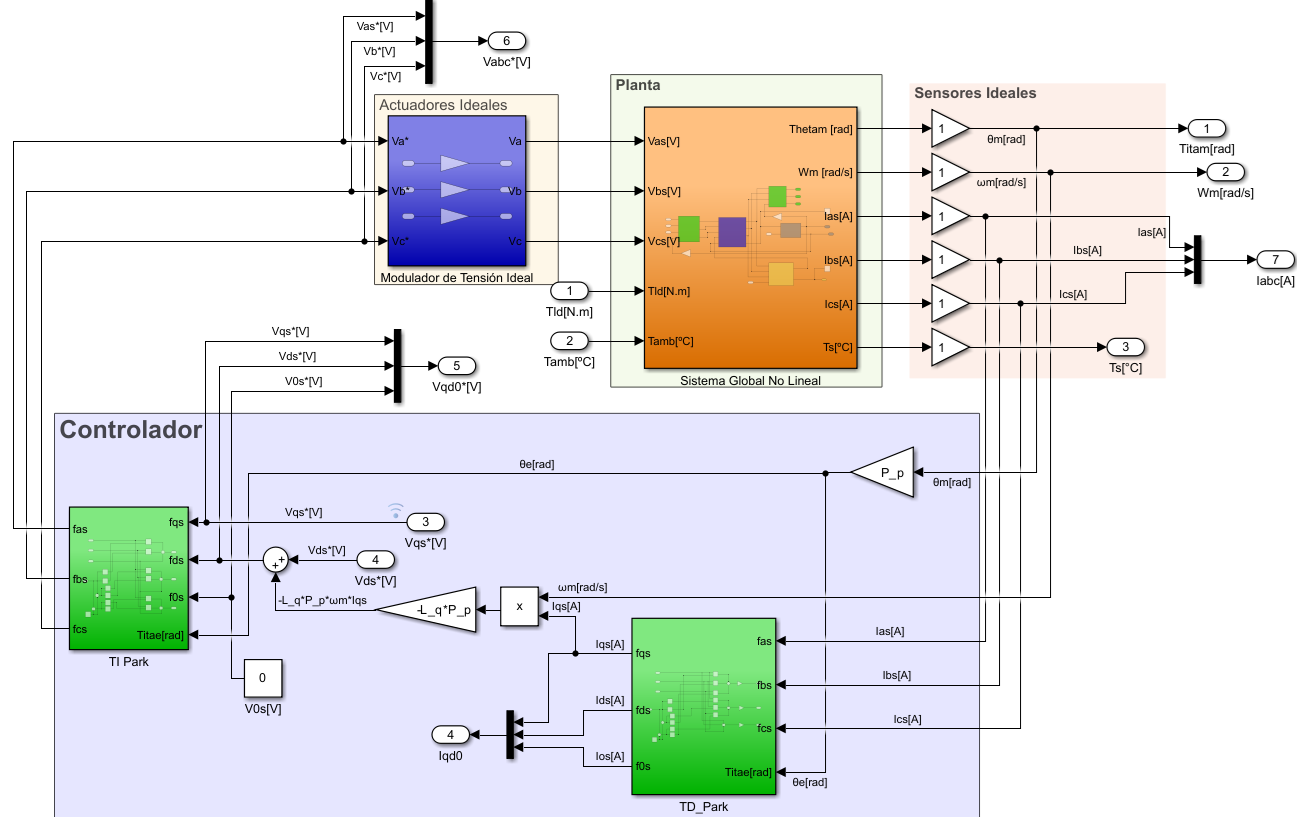
\includegraphics[width=0.9\textwidth]{Imagenes/BloquesLinealizacionRealimentacionNoLineal.png}
    \caption{Diagrama de bloques del sistema linealizado por realimentación parcial de estados mediante un controlador parcial externo.}
    \label{fig:BloquesControladorParcialNoLineal}
\end{figure}
\begin{figure}[H]
    \centering
    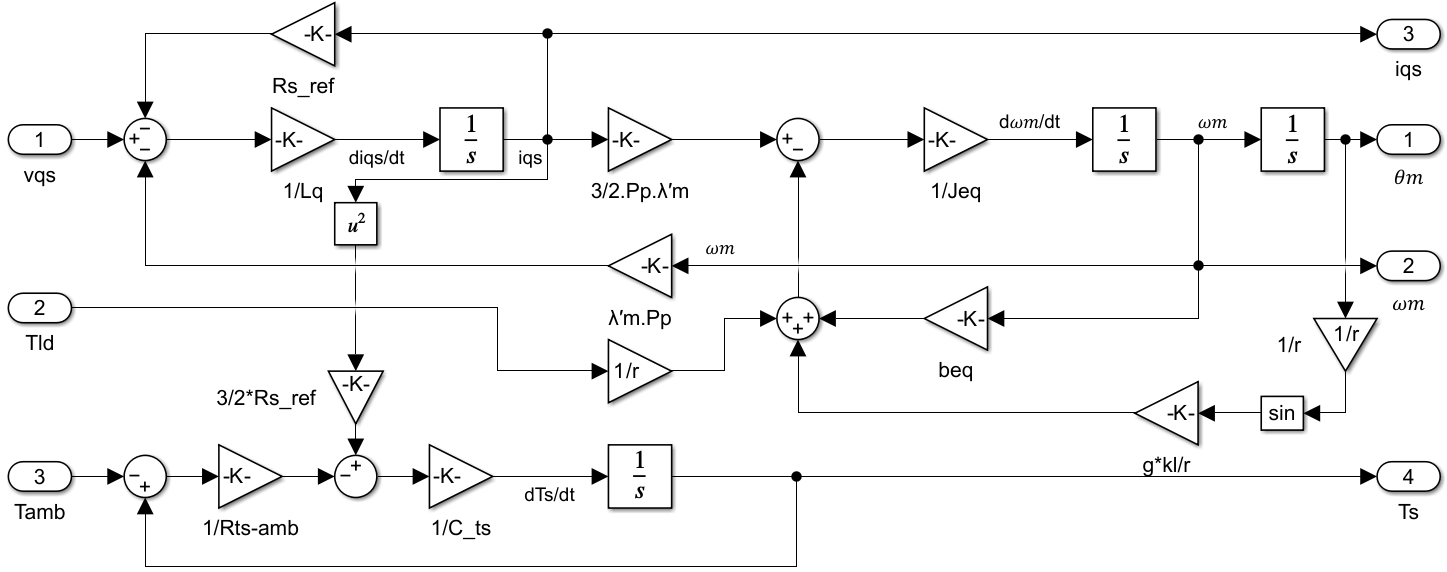
\includegraphics[width=0.9\textwidth]{Imagenes/SistEqLTI.png}
    \caption{Diagrama de bloques de estado modelo LTI equivalente.}
    \label{fig:SistEqLTI}
\end{figure}

\noindent\textbf{Inversor trifásico de alimentación (modulador de tensión)}
Inversor trifásico de 4 cuadrantes (regenerativo), consistente en un puente trifásico con llaves electrónicas semiconductoras (ej. transistores de potencia MOSFETs ó IGBTs) alimentado desde fuente de CC de tensión constante, conmutado con modulación de ancho de pulso, PWM (existen distintas configuraciones y métodos, con ventajas y desventajas).
A continuación se muestra el \textbf{Modelo instantáneo promediado equivalente} de \textit{tensiones sintetizadas de salida} (componente fundamental, sin armónicos): sistema trifásico de tensiones de fase en bornes de fase de estator, senoidales de secuencia positiva abc, equilibrado o balanceado (igual módulo, desfasaje 120° eléctricos), variable en Módulo $V_{st}(t)$ y Frecuencia $\omega_e(t)$:

\begin{equation}
\left\{
\begin{aligned}
v_{as}(t) &= \sqrt{2}\frac{V_{st}(t)}{\sqrt{3}}\cos(\theta_{ev}(t)) \\
v_{bs}(t) &= \sqrt{2}\frac{V_{st}(t)}{\sqrt{3}}\cos(\theta_{ev}(t) - \frac{2\pi}{3}) \\
v_{cs}(t) &= \sqrt{2}\frac{V_{st}(t)}{\sqrt{3}}\cos(\theta_{ev}(t) + \frac{2\pi}{3}) \\
\omega_e(t) &\equiv 2\pi.f_e(t) \equiv \frac{d\theta_{ev}(t)}{dt} \Leftrightarrow \theta_{ev}(t) = \int_0^t \omega_e(\xi).d\xi + \theta_{ev}(0)
\end{aligned}
\right.
\end{equation}
\textbf{Parámetros variables:}
$V_{sl}(t)$ y $\omega_e(t) \equiv 2\pi.f_e(t)$ pueden variarse a voluntad (dentro de ciertos límites) mediante el control vectorial con modulación PWM.

\textbf{Especificaciones de operación} (valores límite, no sobrepasar):
\begin{itemize}
\item Módulo de tensión de línea: $V_{st} = [0.0 ... 48] V_{ca rms}$
\item Frecuencia sincrónica: $f_e = [-330.0 ... 0.0 ... +330.0] Hz$
\end{itemize}
Signo $\pm$ de $f_e$: determina secuencia de fases positiva (abc) ó negativa (acb) y por consiguiente, el sentido de giro $\pm$ del campo magnético rotante y del rotor.

\noindent\textbf{Sensores de retroalimentación}

El sistema cuenta con los siguientes dispositivos físicos y sus canales de medición y acondicionamiento:
\begin{itemize}
\item 1 sensor de posición angular (codificador incremental o ``encoder'') montado en el eje de motor, asumiendo proceso de ``homing'' y decodificación idealizados $\rightarrow$ variable medida: $\theta_m(t)$, posición angular absoluta ``rectificada'' (al girar más de una revolución); tal que $\theta_l(t) = \frac{1}{r}\theta_m(t)$ y ajuste $\theta_m = 0$ (Origen o ``Home'') para $\theta_l = 0$.
\item 3 sensores de corriente instantánea de fase, montados en salida trifásica del inversor hacia bornes del estator $\rightarrow$ variables medidas: $i_{as}(t), i_{bs}(t), i_{cs}(t)$.
\item 1 sensor de temperatura (ej. RTD) en bobinado de estator $\rightarrow$ variable medida: $T^\circ_s(t)$, para monitoreo de calentamiento y estimación de resistencia de estator $R_s\left(T^\circ_s(t)\right)$.

\end{itemize}

\noindent\textbf{Modelo de la dinámica residual}

Con el propósito de modelar la dinámica residual equivalente para $i^r_{ds}(t)$ en el caso general donde no se cumpla la hipótesis asumida para el estado inicial de $i^r_{ds}(t)$ se aplica la ley de control mínima encontrada para $v^r_{ds}(t)$ de la ecuación de estado.
Es así que llegamos a la siguiente EDO que modela el comportamiento de la corriente $i^r_{ds}(t)$:
\begin{equation}
\frac{d i_{ds}^r(t)}{dt} = \frac{1}{L_d} \Big( \cancel{v_{ds}^r(t)} - R_s(t) i_{ds}^r(t) + \cancel{L_q i_{qs}^r(t) P_p \cdot \omega_m(t)} \Big)
\end{equation}
\begin{equation}
L_d \cdot\frac{di^r_{ds}}{dt}(t) + R_s(t)\cdot i^r_{ds}(t) = 0 \quad \rightarrow \quad \frac{di^r_{ds}}{dt}(t) = \frac{1}{L_d}\left[-R_s(t)\cdot i^r_{ds}(t)\right]
\end{equation}
Al resolver esta ecuación encontramos que:
\begin{equation}
i^r_{ds}(t) = i^r_{ds}(0)\cdot e^{-\frac{R_s(t)}{L_d}\cdot t}
\end{equation}
Analizando esta expresión vemos que la corriente decae exponencialmente. Es así que el error de la dinámica residual es debido a un valor inicial de la corriente distinta de cero ``$i^r_{ds}(0) \neq 0$'', lo cual genera un acoplamiento en el eje q y produce un comportamiento no lineal del sistema que desaparecerá al cabo del tiempo, afectando la respuesta natural del sistema pero no así en régimen forzado y es por dicha razón que se puede despreciarlo.
\begin{equation}
\label{eq:acoplamiento_residual_NL}
v^r_{qs}(t) = L_q\cdot \frac{di^r_{qs}}{dt}(t) + R_s(t)\cdot i^r_{ds}(t) + \lambda'_m\cdot P_p\cdot\omega_m(t) + \boldsymbol{L_d\cdot P_p\cdot\omega_m(t)\cdot i^r_{ds}(t)}
\end{equation}
Si incorporamos esta dinámica residual, despreciando el acoplamiento residual NL con el eje q, al modelo LTI equivalente:
\begin{equation}
\left\{
\begin{aligned}
\frac{d\theta_m}{dt}(t) &= \omega_m(t) \\[1ex]
\frac{d\omega_m}{dt}(t) &= \frac{1}{J_{eq}}\left[\frac{3}{2}P_p\lambda^r_mi^r_{qs}(t) - b_{eq}\omega_m(t) - \frac{1}{r}T_{ld}(t) - \frac{g \cdot k_l}{r} \sin\Bigg(\frac{\theta_m(t)}{r}\Bigg)\right] \\[1ex]
\frac{di^r_{qs}}{dt}(t) &= \frac{1}{L_q}\left[v^r_{qs}(t) - R_si^r_{qs}(t) - \lambda^r_mP_p\omega_m(t)\right] \\[1ex]
\frac{di^r_{ds}}{dt}(t) &= -\frac{1}{L_d}R_s\cdot i^r_{ds}(t) \\[1ex]
\frac{d T_s(t)}{dt} &= \frac{1}{C_{ts}} \Bigg[ \frac{3}{2} R_s \cdot \big(i_{qs}^r(t)^2+i_{ds}^r(t)^2\big) - \frac{1}{R_{ts-amb}} \big( T_s(t) - T_{amb}(t) \big) \Bigg]
\end{aligned}
\right.
\label{eq:sistema_LTI_aumentado}
\end{equation}

\noindent\textbf{Restricción o Ley de Control complementaria mínima}

Se puede implementar una Restricción o Ley de Control complementaria mínima en el eje q para eliminar completamente este acoplamiento residual NL aún en régimen natural
y obtener un modelo equivalente completamente lineal, independiente del estado inicial de
\(i^r_{ds}(t)\). Para ello, se realimenta el término no lineal \(L_d\cdot P_p\cdot\omega_m(t)\cdot i^r_{ds}(t)\) de la Ec.~\ref{eq:acoplamiento_residual_NL} en la entrada \(v^r_{qs}\) del sistema. 

\begin{equation}
v^r_{qs}(t) + \cancel{\boldsymbol{L_d\cdot P_p\cdot\omega_m(t)\cdot i^r_{ds}(t)}} = L_q\cdot \frac{di^r_{qs}}{dt}(t) + R_s(t)\cdot i^r_{qs}(t) + \lambda'_m\cdot P_p\cdot\omega_m(t) + \cancel{\boldsymbol{L_d\cdot P_p\cdot\omega_m(t)\cdot i^r_{ds}(t)}}
\end{equation}
Agregamos esta realimentación al controlador parcial de la figura~\ref{fig:BloquesControladorParcialNoLineal}:

\begin{figure}[H]
    \centering
    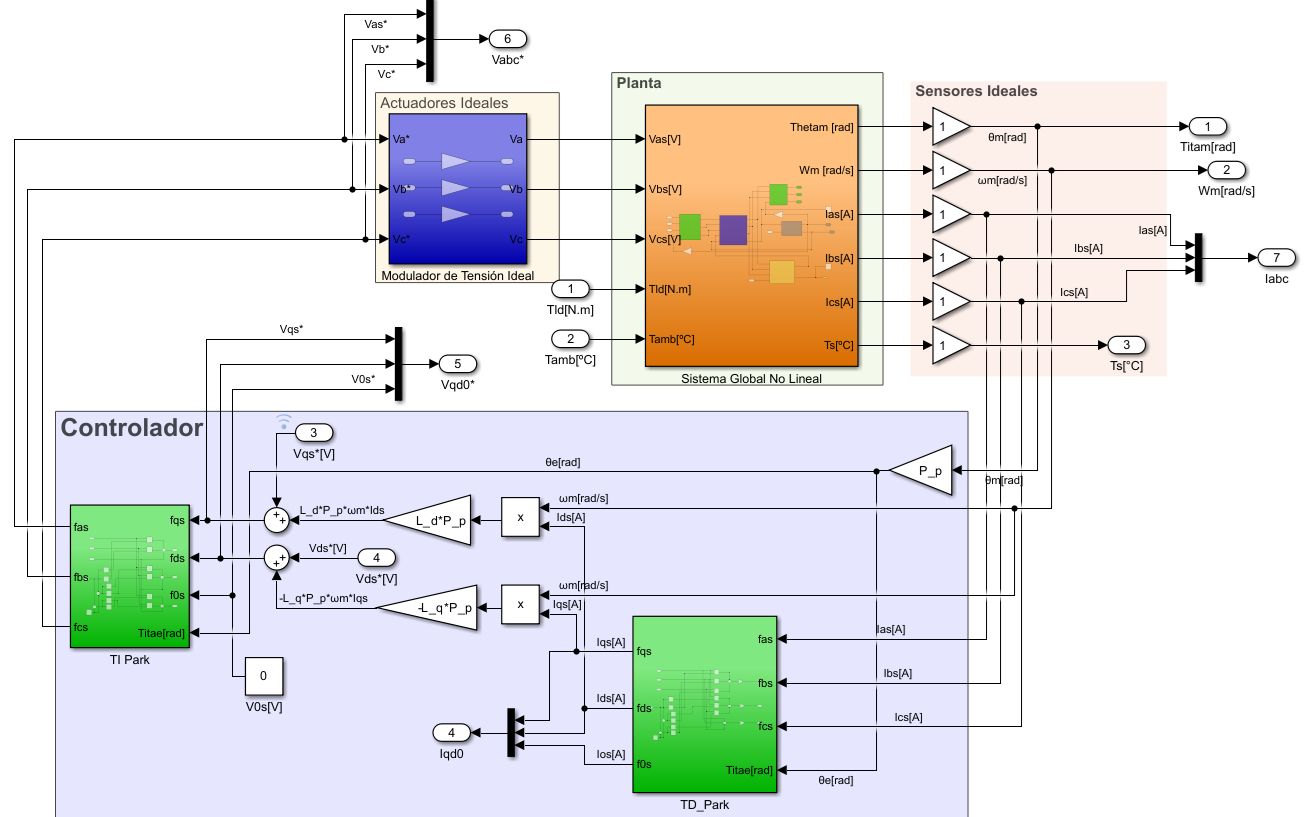
\includegraphics[width=0.9\textwidth]{Imagenes/BloquesLinealizacionRealimentacionNoLinealDesacoplo.png}
    \caption{Implementación de Ley de Control complementaria mínima en el eje q mediante el controlador parcial.}
    \label{fig:BloquesControladorParcialNoLinealDesacoplo}
\end{figure}

En la Figura~\ref{fig:diagrama_sistema_LTI_aumentado} se puede observar el sistema LTI aumentado correspondiente al sistema de ecuaciones~\eqref{eq:sistema_LTI_aumentado}. La diferencia entre este modelo con el modelo Global No Lineal con las leyes de control para desacoplar los canales de flujo magnético y torque, es que en el modelo LTI aumentado no se considera la variación de la resistencia con la temperatura \(T^\circ_s(t)\). Esto provocará leves diferencias en las curvas de las simulaciones de ambos modelos que se analizarán más adelante.

\begin{figure}[H]
    \centering
    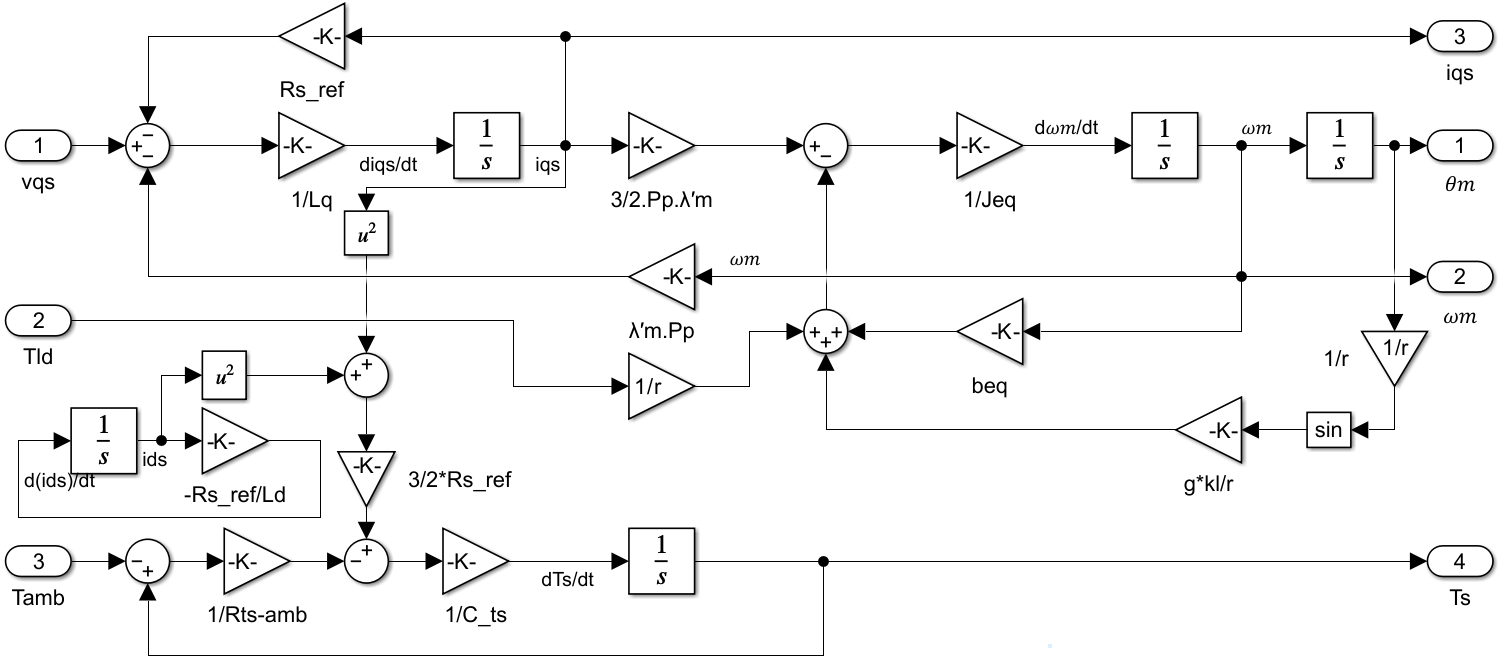
\includegraphics[width=0.9\textwidth]{Imagenes/SistEqLTI_aumentado.png}
    \caption{Diagrama de bloques desagregado del sistema LTI aumentado.}
    \label{fig:diagrama_sistema_LTI_aumentado}
\end{figure}


\noindent\textbf{Modelo Dinámico LTI Equivalente Aumentado vs. Modelo Dinámico Global LPV forzando \(I^r_{dso}\equiv 0 \)}

\textbf{Aspectos principales}
\begin{itemize}
    \item El modelo dinámico global LPV para el caso general ``\(i^r_{ds} \neq 0\)'' representa mejor al sistema real, ya que se tiene un espacio con mayor cantidad de puntos de operación.
    \item El modelo dinámico LTI equivalente aumentado es un caso particular del modelo dinámico global LPV, en donde \(i^r_{ds} = 0\). Realizar esta simplificación implica reducir el espacio de puntos de operación, pero presenta como ventaja un modelo con mucha mayor simplicidad en comparación con el modelo dinámico global LPV.
    \item El modelo dinámico global LPV considera la variación de \(R_{s}(T^\circ_{s}(t))\), en cambio el modelo dinámico LTI equivalente aumentado toma la simplificación de considerar \(R_{s}\) constante.
\end{itemize}
Podemos ver la similitud entre el modelo dinámico global LPV presentado en la (Ec.~\ref{eq:SistemaGlobalLPV}), considerando \(I_{dsr_o} \equiv 0\) y el sistema LTI mostrado en la (Ec.~\ref{eq:sistema_LTI_aumentado}). Más adelante, en las simulaciones, se observará que ambos modelos presentan respuestas dinámicas similares.

\textbf{Análisis del comportamiento del sistema frente a variaciones en ``\(i^r_{ds}\)''}

Por otro lado, como la corriente directa está orientada en el mismo sentido que el campo
principal de la máquina, su variación tiene un efecto en el torque electromagnético $T_{m}$ y la velocidad de rotación
Al primer análisis lo realizamos con respecto al par electromagnético, recordando Ec.~\ref{eq:SubsistemaElectromagnetico}:
 \begin{equation*}
     T_m(t) = \frac{3}{2} P_p [\lambda'^r_m + (L_d - L_q) i_{ds}^r(t)] i_{qs}^r(t).
 \end{equation*}

\begin{itemize}
    \item \textbf{Corriente directa nula (\(i^r_{ds}(t) = 0\))}: Sólo existe flujo concatenado por imanes permanentes (\(\lambda'^r_m\)).
    
    \item \textbf{Reforzamiento de Campo (\(i^r_{ds}(t) > 0\))}: Sabemos que para motores de polos salientes \(L_d > L_q\) , entonces cuando \(i^r_{ds}(t)\) toma valores más positivos, el campo
    magnético principal se refuerza aumentando el torque en el motor. 
    
    \item \textbf{Debilitamiento de Campo (\(i^r_{ds}(t) < 0\))}: En este caso, según la Ec.~\ref{eq:SubsistemaElectromagnetico}, el torque disminuye debido al término \((L_d - L_q)i^r_{ds}(t)\).
\end{itemize}

Ahora analizando lo que pasa con la velocidad, recordando (Ec.~\ref{eq:ExpresionIds}):
 \begin{equation*}
     \frac{d i_{ds}^r(t)}{dt} = \frac{1}{L_d} \Big( v_{ds}^r(t) - R_s(t) i_{ds}^r(t) + L_q i_{qs}^r(t) P_p \cdot \omega_m(t) \Big) = 0 \rightarrow \omega_m(t) = \frac{-v^r_{ds}(t) + R_s(t).i^r_{ds}(t)}{L_q.i^r_{qs}(t).P_p}
 \end{equation*}

\begin{itemize}
    \item \textbf{Corriente directa nula (\(i^r_{ds}(t) = 0\))}: El flujo concatenado está afectado únicamente por los imanes permanentes, y el motor alcanza un estado de equilibrio dinámico entre el par motor y su velocidad.
    
    \item \textbf{Reforzamiento de Campo (\(i^r_{ds}(t) > 0\))}: La velocidad del motor disminuye (ya que el término positivo $R_s(t).i^r_{ds}(t)$ se opone al término negativo $-v^r_{ds}(t)$). 
    
    \item \textbf{Debilitamiento de Campo (\(i^r_{ds}(t) < 0\))}: En este caso, pasa lo contrario al caso anterior con respecto al término $R_s(t).i^r_{ds}(t)$, y la velocidad del motor aumenta.
\end{itemize}


\textbf{Migración de Propiedades Dinámicas}

La variación de \(I_{dsr_o}\) afecta las propiedades dinámicas del sistema LPV, como la estabilidad y el tiempo de asentamiento. En el debilitamiento de campo, el sistema responde más rápidamente pero con menor torque, mientras que en el reforzamiento de campo, el aumento del torque mejora la estabilidad pero puede introducir sobreimpulsos si no se controla adecuadamente.\\



\textbf{Análisis de Variación de Parámetros en sistema LPV}\\
\textbf{Migración de Propiedades ante Variación de \( i_{ds} \)}

Para comprender cómo la corriente directa del estator (\( i_{ds} \)) afecta la dinámica del sistema, se realizó un análisis de variación de \( i_{ds} \) dentro de un rango \([i_{ds}^{\text{init}} - 1,\ i_{ds}^{\text{init}} + 1]\), donde \( i_{ds}^{\text{init}} \) es el valor inicial de la corriente directa. Este análisis permite observar cómo cambian las posiciones de los polos del sistema en el plano \( s \), influyendo en su estabilidad y respuesta transitoria.

\textbf{Resultados de la Variación de \( i_{ds} \)}

A continuación, se presentan los resultados obtenidos para diferentes valores de \( i_{ds} \). Cada fila muestra 6 autovalores del sistema para un valor dado de \( i_{ds} \):

\begin{table}[H]
    \centering
    \label{tab:variacion_i_ds}
    \begin{tabular}{|c|c|}
        \hline
        \textbf{i\_ds [A]} & \textbf{Autovalores (6 en total)} \\
        \hline
        -1.500 & $-0.1+0.0j \quad -88.4+54.6j \quad -88.4-54.6j \quad -154.5+0.0j \quad -0.0+0.0j \quad -1275.0+0.0j$ \\
        \hline
        -1.155 & $-0.1+0.0j \quad -88.4+85.0j \quad -88.4-85.0j \quad -154.5+0.0j \quad -0.0+0.0j \quad -1275.0+0.0j$ \\
        \hline
        -0.810 & $-0.1+0.0j \quad -88.4+107.7j \quad -88.4-107.7j \quad -154.5+0.0j \quad -0.0+0.0j \quad -1275.0+0.0j$ \\
        \hline
        -0.466 & $-0.1+0.0j \quad -88.5+127.0j \quad -88.5-127.0j \quad -154.5+0.0j \quad -0.0+0.0j \quad -1275.0+0.0j$ \\
        \hline
        -0.121 & $-0.1+0.0j \quad -88.5+144.3j \quad -88.5-144.3j \quad -154.5+0.0j \quad -0.0+0.0j \quad -1275.0+0.0j$ \\
        \hline
         0.224 & $-0.0+0.0j \quad -88.5+160.1j \quad -88.5-160.1j \quad -154.5+0.0j \quad -0.0+0.0j \quad -1275.0+0.0j$ \\
        \hline
    \end{tabular}
    \caption{Variación de los 6 autovalores ante cambios en \( i_{ds} \)}
\end{table}

\textbf{Migración de Polos}

En la Figura \ref{fig:migracion_polos_i_ds} se ilustra el diagrama de polos del sistema ante la variación de \( i_{ds} \). Al incrementar \( i_{ds} \) dentro del rango considerado, se observa principalmente un cambio en la parte imaginaria de los polos dominantes complejos conjugados, pasando de valores imaginarios menores (\(\pm 54.6j\)) hacia valores mayores (\(\pm 160.1j\)). Esto sugiere un incremento en la frecuencia de oscilación del sistema a medida que \( i_{ds} \) aumenta.

\begin{itemize}
    \item \textbf{Polos Complejos Conjugados Principales (\(-88.4 \pm bj\) y \(-88.5 \pm bj\))}: A medida que \( i_{ds} \) aumenta, la parte imaginaria de estos polos también aumenta, lo que indica una mayor frecuencia de oscilación. La parte real, sin embargo, permanece en torno a \(-88.4\) a \(-88.5\), indicando que la amortiguación y la estabilidad global del sistema no cambian de forma significativa.

    \item \textbf{Polos Reales:}  
    Algunos polos reales, como el ubicado en \(-154.5+0.0j\), permanecen inalterados ante la variación de \( i_{ds} \), lo que sugiere modos muy amortiguados y poco sensibles a esta corriente.

    \item \textbf{Otros Modos Rápidos:}  
    El polo extremadamente negativo \(-1275.0+0.0j\) tampoco se modifica, indicando un modo muy rápido e independiente de \( i_{ds} \).
\end{itemize}

\begin{figure}[H]
    \centering
    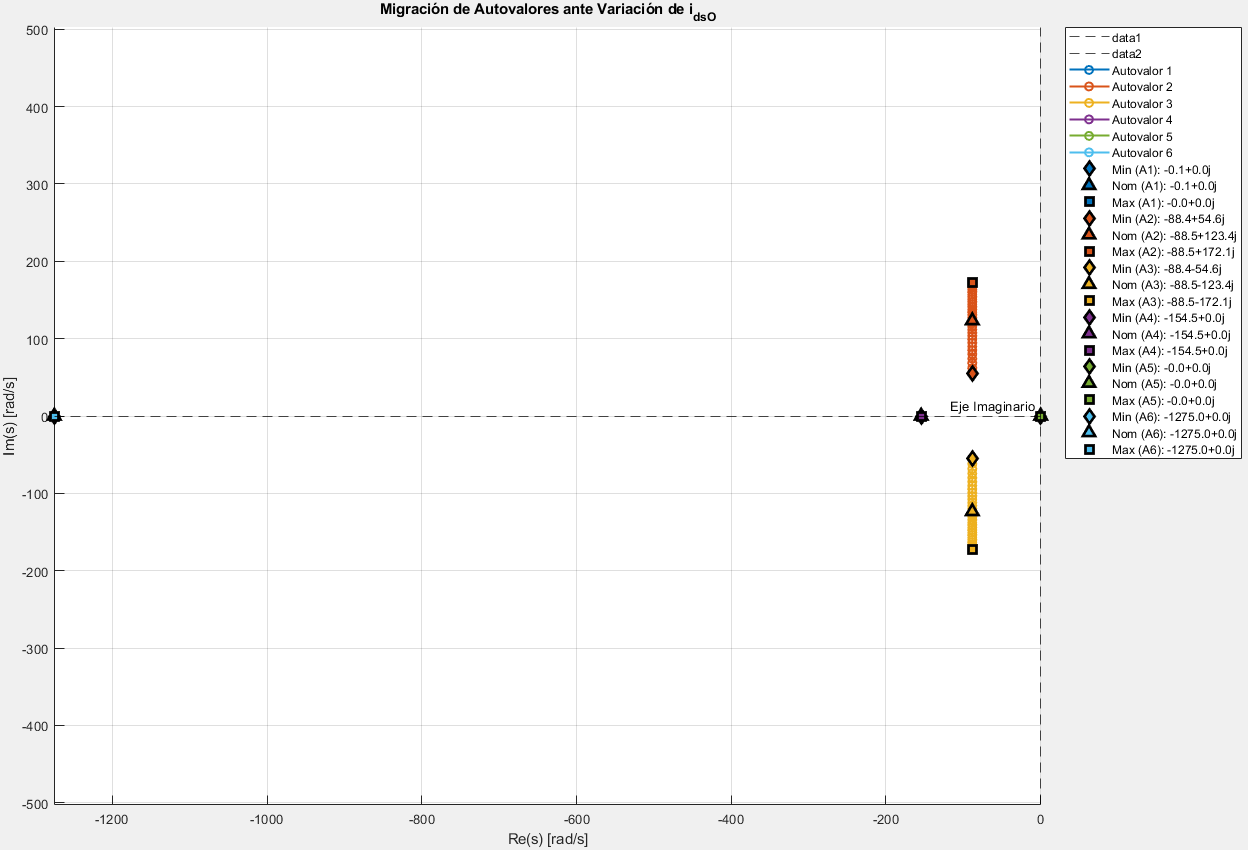
\includegraphics[width=0.55\textwidth]{Imagenes/MigracionLPV_1.png}
    \caption{Migración de Polos ante Variación de \( i_{ds} \)}
    \label{fig:migracion_polos_i_ds}
\end{figure}

\begin{figure}[H]
    \centering
    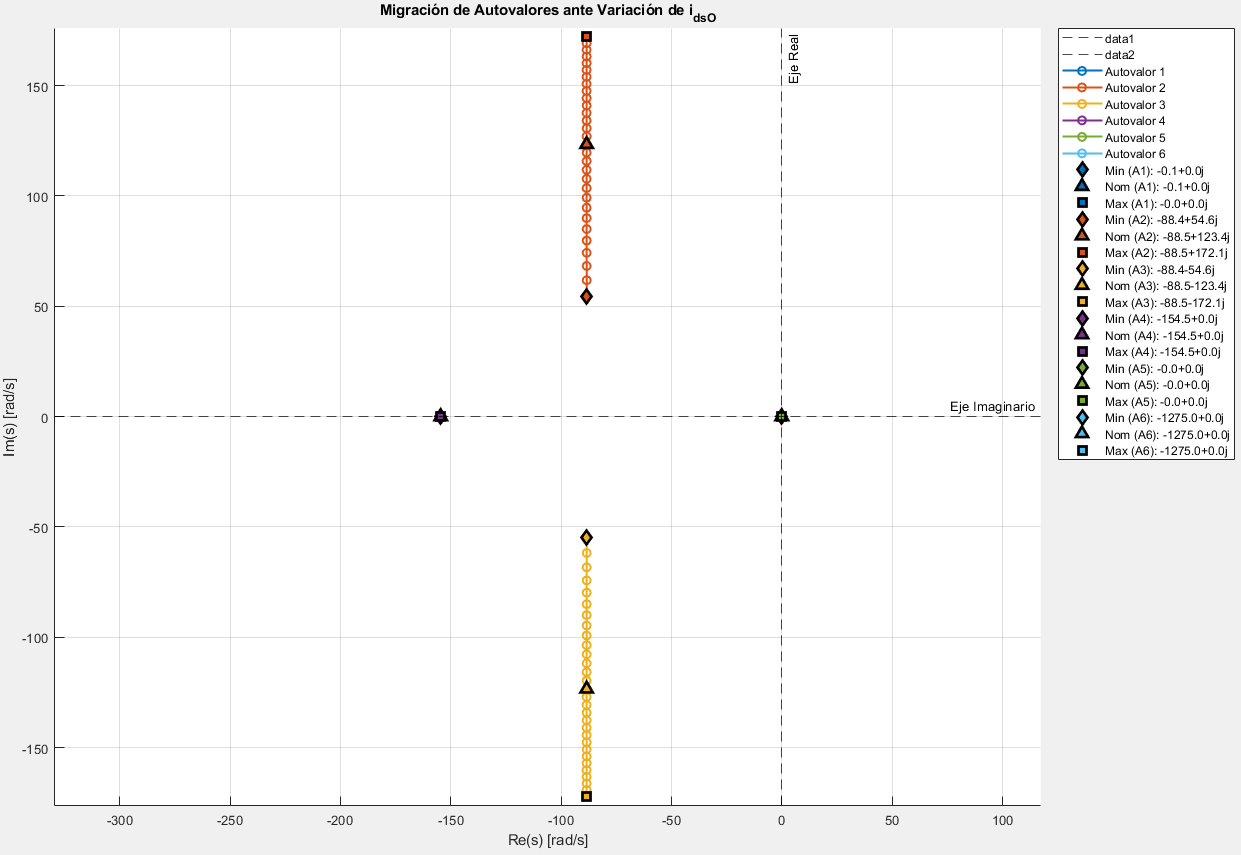
\includegraphics[width=0.55\textwidth]{Imagenes/MigracionLPV_2.png}
    \caption{Acercamiento: Migración de Polos ante Variación de \( i_{ds} \)}
    \label{fig:migracion_polos_i_ds}
\end{figure}

\textbf{Interpretación de Resultados}

El análisis sugiere que la variación de \( i_{ds} \) afecta principalmente la frecuencia de oscilación de los polos complejos conjugados, incrementando su parte imaginaria, pero sin alterar significativamente su parte real. Por ello, la estabilidad y el amortiguamiento del sistema permanecen prácticamente constantes.

En consecuencia, \( i_{ds} \) ejerce un efecto moderado sobre la dinámica del sistema, modificando de manera sutil la respuesta transitoria sin comprometer la estabilidad ni las características esenciales del mismo.


\newpage

\noindent\textbf{Funciones de Transferencia para el Modelo LTI Equivalente Aumentado}

Para obtener las funciones de transferencia desde las entradas \( v_{qsr}(t) \) y \( T_l(t) \) hacia la salida \( \theta_m(t) \) para el modelo LTI equivalente aumentado, partimos del sistema completo y aplicamos las siguientes consideraciones:

\begin{itemize}
    \item \textbf{Subsistema Térmico Desacoplado}: Consideramos \( R_s(t) = R_s \) constante.
    \item \textbf{Control Vectorial Orientado a Campo}: Se asume \( i_{ds}^r(t) = 0 \).
    \item \textbf{Condiciones Iniciales Nulas}: Todas las condiciones iniciales se consideran nulas para la aplicación de la transformada de Laplace.
\end{itemize}

\textbf{Definición de \( T_l(t) \)}

Definimos la variable \( T_l(t) \) como:

\[
T_l(t) = T_{ld}(t) + g \cdot k_l \sin\left(\frac{\theta_m(t)}{r}\right)
\]

Esta definición agrupa los términos no lineales y dependientes de \( \theta_m(t) \).

\textbf{Sistema Reducido con \( T_l(t) \)}

Sustituyendo los términos, el sistema se reduce a:

\[
\left\{
\begin{aligned}
\frac{d\theta_m}{dt}(t) &= \omega_m(t) \\[1ex]
\frac{d\omega_m}{dt}(t) &= \frac{1}{J_{eq}} \left[ \frac{3}{2} P_p \lambda'^r_m i^r_{qs}(t) - b_{eq} \omega_m(t) - \frac{1}{r}\cdot T_l(t) \right] \\[1ex]
\frac{di^r_{qs}}{dt}(t) &= \frac{1}{L_q} \left[ v^r_{qs}(t) - R_s i^r_{qs}(t) - \lambda'^r_m P_p \omega_m(t) \right]
\end{aligned}
\right.
\]


A partir del sistema reducido, derivamos las funciones de transferencia desde las entradas \( v_{qsr}(t) \) y \( T_l(t) \) hacia la salida \( \theta_m(t) \) aplicando la transformada de Laplace con condiciones iniciales nulas.

\textbf{Aplicación de la Transformada de Laplace}

Transformamos las ecuaciones del sistema reducido:

\[
\left\{
\begin{aligned}
s\Theta_m(s) &= \Omega_m(s) \\[1ex]
s\Omega_m(s) &= \frac{1}{J_{eq}} \left[ \frac{3}{2} P_p \lambda'^r_m I^r_{qs}(s) - b_{eq} \Omega_m(s) - T_l(s) \right] \\[1ex]
sI^r_{qs}(s) &= \frac{1}{L_q} \left[ V^r_{qs}(s) - R_s I^r_{qs}(s) - \lambda'^r_m P_p \Omega_m(s) \right]
\end{aligned}
\right.
\]

\textbf{Resolución del Sistema}

1. Resolver para \( I^r_{qs}(s) \):

\[
I^r_{qs}(s) = \frac{V^r_{qs}(s) - \lambda'^r_m P_p \Omega_m(s)}{L_q s + R_s}
\]

2. Sustituir \( I^r_{qs}(s) \) en la segunda ecuación:

\[
s\Omega_m(s) = \frac{1}{J_{eq}} \left[ \frac{3}{2} P_p \lambda'^r_m \cdot \frac{V^r_{qs}(s) - \lambda'^r_m P_p \Omega_m(s)}{L_q s + R_s} - b_{eq} \Omega_m(s) - T_l(s) \right]
\]

3. Reorganizar y resolver para \( \Omega_m(s) \):

\[
\Omega_m(s) = \frac{\frac{3}{2} P_p \lambda'^r_m V^r_{qs}(s) - (L_q s + R_s) T_l(s)}{J_{eq} L_q s^2 + (J_{eq} R_s + b_{eq} L_q) s + \left(b_{eq} R_s + \frac{3}{2} P_p^2 (\lambda'^r_m)^2\right)}
\]

4. Obtener \( \Theta_m(s) \):

\[
\Theta_m(s) = \frac{\Omega_m(s)}{s} = \frac{\frac{3}{2} P_p \lambda'^r_m V^r_{qs}(s) - (L_q s + R_s) T_l(s)}{s \left( J_{eq} L_q s^2 + (J_{eq} R_s + b_{eq} L_q) s + \left(b_{eq} R_s + \frac{3}{2} P_p^2 (\lambda'^r_m)^2 \right) \right)}
\]

\textbf{Funciones de Transferencia}

\[
\Theta_m(s) = G_{V_{qs}}(s) \cdot V^r_{qs}(s) + G_{T_l}(s) \cdot T_l(s)
\]

Donde:
\begin{equation}
G_{V_{qs}}(s) = \frac{\frac{3}{2} P_p \lambda'^r_m}{J_{eq} L_q s^3 + (J_{eq} R_s + b_{eq} L_q) s^2 + \left(b_{eq} R_s + \frac{3}{2} P_p^2 (\lambda'^r_m)^2\right) s}
\end{equation}
\begin{equation}
G_{T_l}(s) = \frac{-(L_q s + R_s)}{J_{eq} L_q s^3 + (J_{eq} R_s + b_{eq} L_q) s^2 + \left(b_{eq} R_s + \frac{3}{2} P_p^2 (\lambda'^r_m)^2\right) s}
\end{equation}

\textbf{Estados Internos no Reflejados en las Funciones de Transferencia}

En el modelo LTI equivalente aumentado completo, existen cinco estados internos:

\begin{itemize}
    \item \( \theta_m(t) \): Posición angular del motor
    \item \( \omega_m(t) \): Velocidad angular del motor
    \item \( i_{qs}^r(t) \): Corriente del eje \( q \)
    \item \( i_{ds}^r(t) \): Corriente del eje \( d \)
    \item \( T_s(t) \): Temperatura del estator
\end{itemize}

Sin embargo, en las funciones de transferencia obtenidas \( G_{V_{qs}}(s) \) y \( G_{T_l}(s) \), sólo se reflejan tres de estos estados (\( \theta_m(t) \), \( \omega_m(t) \) e \( i_{qs}^r(t) \)). Los estados \( i_{ds}^r(t) \) y \( T_s(t) \) no aparecen debido a:

\begin{itemize}
    \item \( i_{ds}^r(t) \): Se mantiene en cero por el control vectorial orientado a campo, y su dinámica está desacoplada del sistema principal.
    \item \( T_s(t) \): Al desacoplar el subsistema térmico y considerar \( R_s \) constante, la temperatura del estator no afecta directamente al modelo eléctrico-mecánico.
\end{itemize}


\subsection{Análisis de Estabilidad a lazo abierto}

\textbf{Determinación de los Autovalores:}

Se determinaron los polos y ceros del sistema a partir de igualar a cero el polinomio característico obtenido de las funciones de transferencia Ec. 52 y Ec. 53. Se puede observar que se puede factorizar un término de \( s \), lo que indica la presencia de un polo en el origen, y luego resolver la ecuación cuadrática resultante para obtener los demás polos. Los valores que satisfacen la igualdad son:

\[
\left\{
\begin{aligned}
s_1 &= 0 \\
s_2 &= -\frac{L_{q}\,b_{\mathrm{eq}}+\sqrt{{J_{\mathrm{eq}}}^2\,{R_{s}}^2 - 6\,J_{\mathrm{eq}}\,L_{q}\,{P_{p}}^2\,{\lambda_{r,m}}^2 - 2\,J_{\mathrm{eq}}\,L_{q}\,R_{s}\,b_{\mathrm{eq}} + {L_{q}}^2\,{b_{\mathrm{eq}}}^2} + J_{\mathrm{eq}}\,R_{s}}{2\,J_{\mathrm{eq}}\,L_{q}} \\
s_3 &= -\frac{L_{q}\,b_{\mathrm{eq}} - \sqrt{{J_{\mathrm{eq}}}^2\,{R_{s}}^2 - 6\,J_{\mathrm{eq}}\,L_{q}\,{P_{p}}^2\,{\lambda_{r,m}}^2 - 2\,J_{\mathrm{eq}}\,L_{q}\,R_{s}\,b_{\mathrm{eq}} + {L_{q}}^2\,{b_{\mathrm{eq}}}^2} + J_{\mathrm{eq}}\,R_{s}}{2\,J_{\mathrm{eq}}\,L_{q}}
\end{aligned}
\right.
\]

Reemplazando los parámetros:
\[
\left\{
\begin{aligned}
s_1 &= 0 \\
s_2 &= -88.5 + 149.9j \ \text{rad/s} \\
s_3 &= -88.5 - 149.9j \ \text{rad/s}
\end{aligned}
\right.
\]


\textbf{Polo en el Origen}

El sistema presenta un polo extra debido a la integración de la velocidad angular para obtener la posición angular. Este polo se ubica en:

\[
s_1 = 0
\]

\textbf{Polos del Subsistema Electromecánico}

Además del polo en el origen, el subsistema electromecánico contribuye con dos polos complejos conjugados que representan los modos dinámicos del sistema. Estos polos se encuentran en:

\[
s_{2,3} = -88.5 \pm 149.9j \ \text{rad/s}
\]

\textbf{Determinación de Ceros}

Al observar las funciones de transferencia \( G_{V_{qs}}(s) \) y \( G_{T_l}(s) \), se puede determinar que:

\begin{itemize}
    \item \( G_{V_{qs}}(s) \) no presenta ceros finitos ya que su numerador es constante.
    \item \( G_{T_l}(s) \) presenta un cero en:
    \[
    z = -\frac{R_s}{L_q} = -175.862 \ \text{rad/s}
    \]
\end{itemize}

\textbf{Frecuencia Natural y Amortiguamiento}

Para determinar la frecuencia natural (\( \omega_n \)) y el factor de amortiguamiento (\( \zeta \)) del sistema, se comparó el polinomio característico obtenido con la forma estándar de un sistema de segundo orden:

\[
(s - p)(s^2 + 2\zeta\omega_n s + \omega_n^2)
\]

De esta comparación, se obtiene:

\[
(s + 0)(s^2 + 176.97s + 30312) 
\]

Entonces:

\[
\omega_n = \sqrt{30312} \approx 174.1 \ \text{rad/s}
\]

\[
\zeta = \frac{176.97}{2 \cdot 174.1} \approx 0.508
\]

\begin{figure}[H]
    \centering
    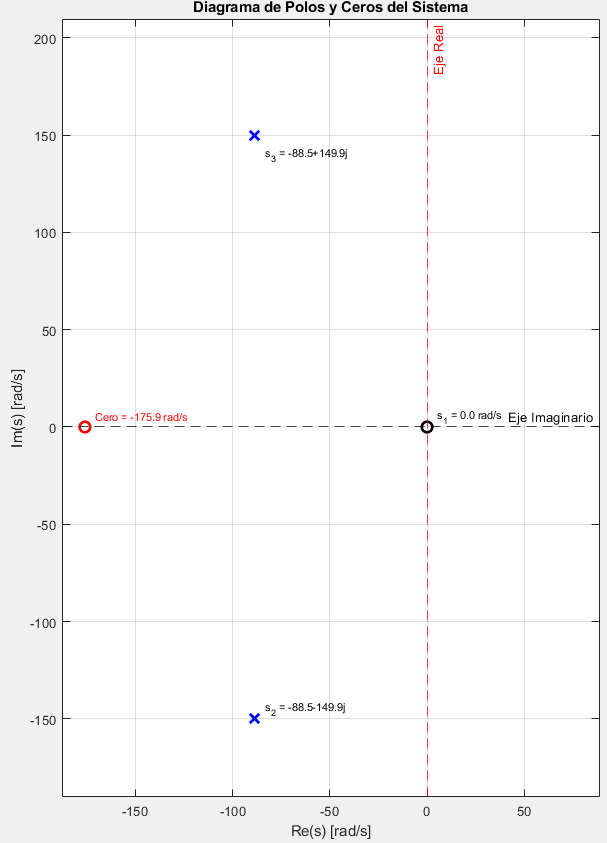
\includegraphics[width=0.5\textwidth]{Imagenes/mapa_polos_ceros.png}
    \caption{Mapa de polos y ceros a lazo abierto}
    \label{fig:polos_ceros}
\end{figure}

Se puede concluir que el sistema es estable, ya que todos sus polos se encuentran en el semiplano izquierdo del dominio de Laplace y presenta un comportamiento subamortiguado.\\


\textbf{Análisis de Variación de Parámetros}\\
\textbf{Migración de Propiedades ante Variación de Rs}

Para comprender cómo la resistencia del estator (\( R_s \)) afecta la dinámica del sistema, se realizó un análisis de variación de \( R_s \) dentro de un rango de \([0.8 \cdot R_s^{\text{ref}}, 1.2 \cdot R_s^{\text{ref}}]\), donde \( R_s^{\text{ref}} \) es el valor nominal de la resistencia. Este análisis permite observar cómo cambian las posiciones de los polos y ceros en el plano \( s \), lo que influye directamente en la estabilidad y el comportamiento transitorio del sistema.

\textbf{Resultados de la Variación de Rs}

A continuación, se presentan los resultados obtenidos para diferentes valores de \( R_s \):

\begin{table}[H]
    \centering
    \label{tab:variacion_Rs}
    \begin{tabular}{|c|c|c|c|c|}
        \hline
        \textbf{Rs [ohms]} & \textbf{Polos} & \textbf{Cero} & \textbf{\(\omega_n\) [rad/s]} & \textbf{\(\zeta\)} \\
        \hline
        0.816 & $s_{2,3} = -70.9 \pm 158.9j$ & -140.69 & 174.0 & 0.41 \\
        \hline
        0.849 & $s_{2,3} = -73.8 \pm 157.6j$ & -146.43 & 174.0 & 0.42 \\
        \hline
        0.883 & $s_{2,3} = -76.6 \pm 156.2j$ & -152.17 & 174.0 & 0.44 \\
        \hline
        0.916 & $s_{2,3} = -79.5 \pm 154.8j$ & -157.92 & 174.0 & 0.46 \\
        \hline
        0.949 & $s_{2,3} = -82.4 \pm 153.3j$ & -163.66 & 174.1 & 0.47 \\
        \hline
        0.983 & $s_{2,3} = -85.3 \pm 151.8j$ & -169.40 & 174.1 & 0.49 \\
        \hline
        1.016 & $s_{2,3} = -88.1 \pm 150.2j$ & -175.14 & 174.1 & 0.51 \\
        \hline
        1.049 & $s_{2,3} = -91.0 \pm 148.4j$ & -180.89 & 174.1 & 0.52 \\
        \hline
        1.082 & $s_{2,3} = -93.9 \pm 146.7j$ & -186.63 & 174.1 & 0.54 \\
        \hline
        1.116 & $s_{2,3} = -96.7 \pm 144.8j$ & -192.37 & 174.2 & 0.56 \\
        \hline
        1.149 & $s_{2,3} = -99.6 \pm 142.9j$ & -198.11 & 174.2 & 0.57 \\
        \hline
        1.182 & $s_{2,3} = -102.5 \pm 140.9j$ & -203.86 & 174.2 & 0.59 \\
        \hline
        1.216 & $s_{2,3} = -105.4 \pm 138.7j$ & -209.60 & 174.2 & 0.60 \\
        \hline
    \end{tabular}
    \caption{Variación de Rs y sus Efectos en Polos y Ceros}
\end{table}

\textbf{Migración de Polos y Ceros}

En la Figura \ref{fig:migracion_polos_ceros} se muestra el diagrama de polos y ceros del sistema a medida que varía \( R_s \). Se observa que:

\begin{itemize}
    \item \textbf{Polos (\( s_{2,3} \)):} A medida que \( R_s \) aumenta, los polos se desplazan hacia la izquierda en el semiplano real, lo que indica una mayor estabilidad del sistema. Además, la parte imaginaria de los polos disminuye ligeramente, lo que sugiere una reducción en la amplitud de las oscilaciones transitorias.
    \item \textbf{Cero del Sistema (\( z \)):} El cero se desplaza hacia la izquierda proporcionalmente a la variación de \( R_s \), lo que afecta la respuesta transitoria del sistema al modificar la relación entre los polos y ceros.
\end{itemize}

\begin{figure}[H]
    \centering
    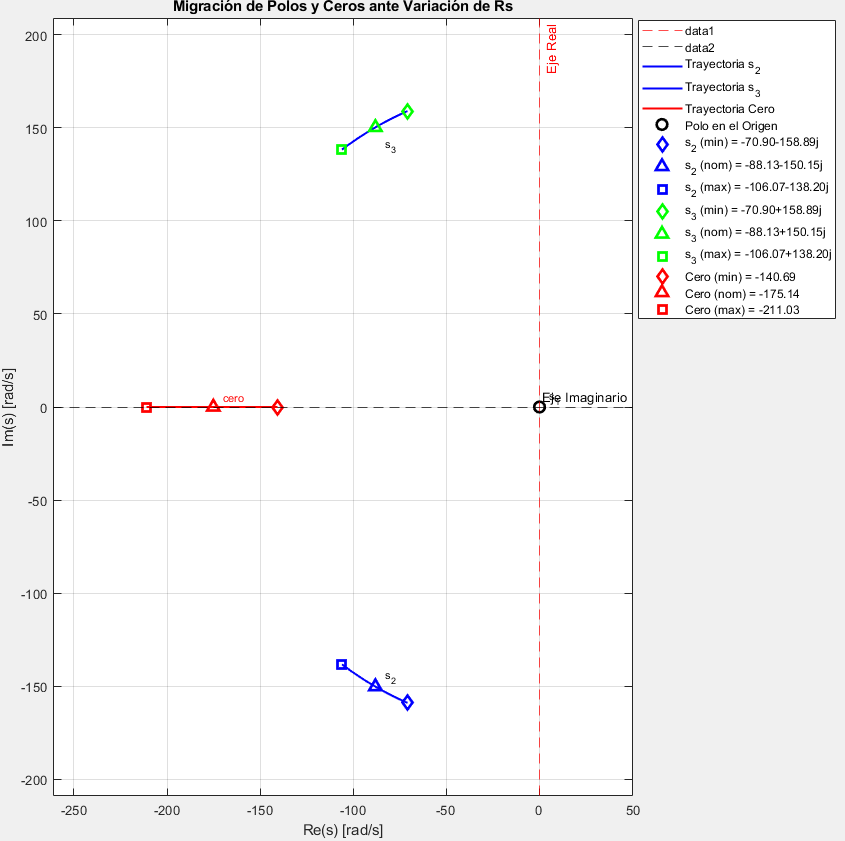
\includegraphics[width=0.55\textwidth]{Imagenes/migracion_polos_ceros.png}
    \caption{Migración de Polos y Ceros ante Variación de \( R_s \)}
    \label{fig:migracion_polos_ceros}
\end{figure}

\textbf{Interpretación de Resultados}

El análisis demuestra que una mayor resistencia del estator (\( R_s \)) contribuye a una mayor estabilidad del sistema al desplazar los polos hacia la izquierda en el plano \( s \). Además, esta variación provoca un aumento en el factor de amortiguamiento (\( \zeta \)), lo que indica que el sistema se vuelve más amortiguado y, por lo tanto, reduce las oscilaciones en su respuesta transitoria. La frecuencia natural (\( \omega_n \)) del sistema permanece aproximadamente constante, lo que implica que la rapidez de la respuesta no se ve significativamente afectada.


\subsection{Análisis de Observabilidad Completa de Estado}

En este análisis, se considera el modelo LTI equivalente aumentado con la matriz de estado \( A \) y las matrices de salida \( C_{\theta} \) y \( C_{\omega} \) correspondientes a las mediciones de la posición \(\theta_m(t)\) y la velocidad angular \(\omega_m(t)\).

La matriz de estado \( A \) y las matrices de salida \( C_{\theta} \) y \( C_{\omega} \) están definidas como sigue:

\[
A = \begin{bmatrix}
0 & 1 & 0 \\
0 & -\frac{b_{\text{eq}}}{J_{\text{eq}}} & \frac{3 P_{p} \lambda'_{m}}{2 J_{\text{eq}}} \\
0 & -\frac{P_{p} \lambda'_{m}}{L_q} & -\frac{R_s}{L_q}
\end{bmatrix}
\]

\[
C_{\theta} = \begin{bmatrix}
1 & 0 & 0
\end{bmatrix}, \quad
C_{\omega} = \begin{bmatrix}
0 & 1 & 0
\end{bmatrix}
\]

Con estas definiciones, procederemos al análisis de la observabilidad del sistema.

\textbf{Observabilidad desde la Salida Medida $\theta_m(t)$}

La matriz de observabilidad \( O_{\theta} \) se construye utilizando la matriz de estado \( A \) y la matriz de salida \( C_{\theta} \), como se define en la siguiente expresión:

\[
O_{\theta} = \begin{bmatrix}
C_{\theta} \\
C_{\theta} A \\
C_{\theta} A^2
\end{bmatrix}
\]

Donde \( C_{\theta} \) es la matriz que mide la posición \(\theta_m(t)\). La matriz resultante es:

\[
O_{\theta} = \begin{bmatrix}
1 & 0 & 0 \\
0 & 1 & 0 \\
0 & -\frac{b_{\text{eq}}}{J_{\text{eq}}} & \frac{3 P_{p} \lambda'_{m}}{2 J_{\text{eq}}}
\end{bmatrix}
\]

El rango de la matriz de observabilidad es 3, lo que indica que el sistema es completamente observable desde la salida medida \(\theta_m(t)\).

\textbf{Observabilidad desde la Salida Medida $\omega_m(t)$}

Para la salida medida de la velocidad angular \(\omega_m(t)\), la matriz de observabilidad \( O_{\omega} \) se construye de manera similar utilizando la matriz de salida \( C_{\omega} \):

\[
O_{\omega} = \begin{bmatrix}
C_{\omega} \\
C_{\omega} A \\
C_{\omega} A^2
\end{bmatrix}
\]

La matriz de observabilidad \( O_{\omega} \) se expresa como:

\[
O_{\omega} = \begin{bmatrix}
0 & 1 & 0 \\
0 & -\frac{b_{\text{eq}}}{J_{\text{eq}}} & \frac{3 P_{p} \lambda'_{m}}{2 J_{\text{eq}}} \\
0 & \frac{b_{\text{eq}}^2}{J_{\text{eq}}^2} - \frac{3 P_{p}^2 (\lambda'_{m})^2}{2 J_{\text{eq}} L_q} & -\frac{3 P_{p} b_{\text{eq}} \lambda'_{m}}{2 J_{\text{eq}}^2} - \frac{3 P_{p} R_s \lambda'_{m}}{2 J_{\text{eq}} L_q}
\end{bmatrix}
\]

El rango de la matriz de observabilidad es 2, lo que indica que el sistema NO es completamente observable desde la salida medida \(\omega_m(t)\). Esto se debe a que por más que se conozca la velocidad del sistema, no es posible obtener la posición del mismo sin conocer la condición inicial de posición. Caso contrario a lo que sucede cuando se conoce la posición del sistema, ya que si se la deriva, se puede llegar a conocer la velocidad del mismo.



\subsection{Análisis de Controlabilidad Completa de Estado}

En este análisis, se estudia la controlabilidad del sistema LTI equivalente aumentado desde la entrada manipulada \( v_{qsr}(t) \), sin considerar la perturbación de la carga mecánica.

La matriz de estado \( A \) y la matriz de entrada \( B \) están definidas como sigue:

\[
A = \begin{bmatrix}
0 & 1 & 0 \\
0 & -\frac{b_{\text{eq}}}{J_{\text{eq}}} & \frac{3 P_{p} \lambda'_{m}}{2 J_{\text{eq}}} \\
0 & -\frac{P_{p} \lambda'_{m}}{L_q} & -\frac{R_s}{L_q}
\end{bmatrix}, \quad
B = \begin{bmatrix}
0 \\
0 \\
\frac{1}{L_q}
\end{bmatrix}
\]

A partir de las matrices de estado \( A \) y de entrada \( B \), se construye la matriz de controlabilidad \( C \), que se expresa como:

\[
C = \begin{bmatrix}
B & A B & A^2 B
\end{bmatrix}
\]

La matriz de controlabilidad \( C \) resultante es:

\[
C = \begin{bmatrix}
0 & 0 & \frac{3 P_p \lambda'_{m}}{2 J_{\text{eq}} L_q} \\
0 & \frac{3 P_p \lambda'_{m}}{2 J_{\text{eq}} L_q} & -\frac{\frac{3 P_p b_{\text{eq}} \lambda'_{m}}{2 J_{\text{eq}}^2} + \frac{3 P_p R_s \lambda'_{m}}{2 J_{\text{eq}} L_q}}{L_q} \\
\frac{1}{L_q} & -\frac{R_s}{L_q^2} & \frac{\frac{R_s^2}{L_q^2} - \frac{3 P_p^2 \lambda^{'2}_{m}}{2 J_{\text{eq}} L_q}}{L_q}
\end{bmatrix}
\]

El rango de la matriz de controlabilidad es 3, lo que indica que el sistema \textbf{es completamente controlable} desde la entrada manipulada \( v_{qsr}(t) \). Esto implica que, con esta única entrada de control, es posible controlar todos los estados del sistema.

Dado que el rango de la matriz de controlabilidad es igual al número de estados del sistema, no se requiere ninguna entrada adicional para lograr la controlabilidad completa. El sistema es capaz de ser controlado de manera óptima desde \( v_{qsr}(t) \), lo que simplifica el diseño y la implementación del controlador.





\newpage
\subsection{Simulación dinámica}
\subsubsection{Respuesta del estado interno}
\label{sec:respuesta_estado_interno_simulaciónDT}
A continuación, se realizará la simulación dinámica en el dominio del tiempo, comparando el modelo NL completo desacoplado con Ley de control NL vs LTI equivalente aumentado. En primer lugar se considera un estado inicial \(i^r_{ds}(0) = 0A\) y luego se comparará con el estado inicial \(i^r_{ds} = \pm 5A\). 
Se analiza la respuesta del estado interno $\{\theta_m(t);\omega_m(t);i^r_{qd0s}(t);T^\circ_s(t)\}$ (y \(v^r_{ds}\) forzada) a pulso de consigna de tensión de estator en eje q, superpuesto con doble pulso de torque de carga y con una temperatura ambiente de 25°C. En la imagen~\ref{fig:EntradasSimulacionDT} se observan estos escalones de entradas.

\begin{figure}[H]
    \centering
    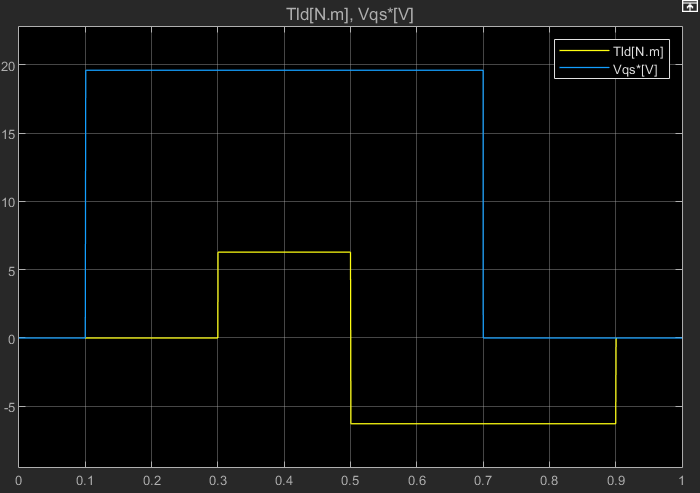
\includegraphics[width=0.45\textwidth]{Imagenes/EntradasTdVq.png}
    \caption{Consignas de Tensión \(V^{r*}_{qs}\) y Torque de carga \(T_{ld}\).}
    \label{fig:EntradasSimulacionDT}
\end{figure}

En la figura~\ref{fig:VelPosTorqueAlineados} se observa que la velocidad empieza a oscilar en el instante 0.1s hasta establecerse en un valor luego de que la tensión \(V^{r*}_{qs}\) pegue un salto a 19.596V, este escalón perdura hasta el instante 0.7s y vuelve a 0V. Luego se observa también para los instantes 0.3s, 0.5s y 0.9s cómo los cambios en la perturbación modifican la velocidad angular de equilibrio del sistema.

\begin{figure}[H]
    \centering
    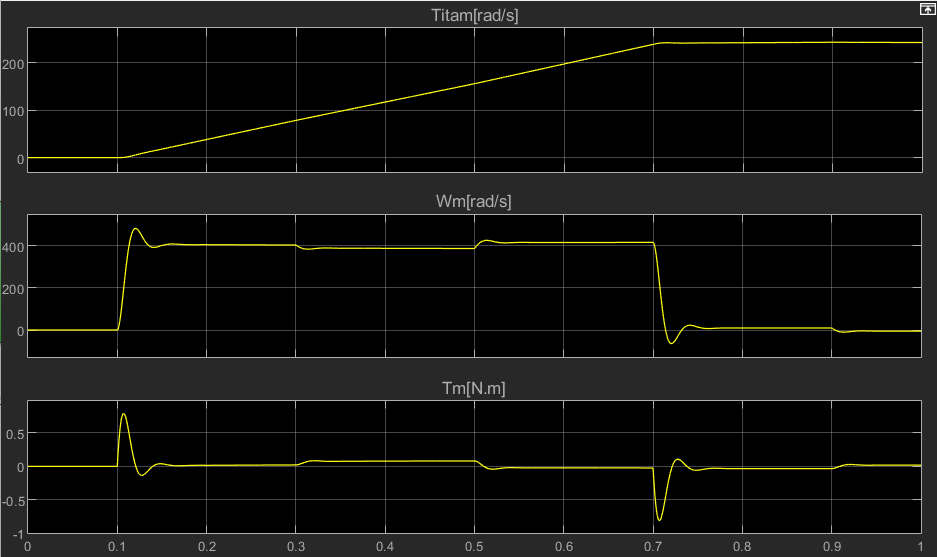
\includegraphics[width=0.7\textwidth]{Imagenes/VelPosTorqueAlineados.png}
    \caption{Curvas de posición angular, velocidad angular y torque electromagnético.}
    \label{fig:VelPosTorqueAlineados}
\end{figure}



En la Figura~\ref{fig:TemperaturaEstatorDT} se observa como varía la temperatura de los bobinados del estator, considerando una perturbación de la temperatura ambiente igual a 25°C.
\begin{figure}[H]
    \centering
    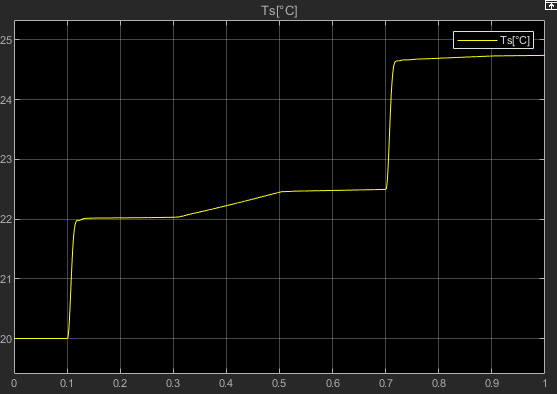
\includegraphics[width=0.55\textwidth]{Imagenes/TemperaturaEstatorDT.png}
    \caption{Temperatura de bobinados del estator.}
    \label{fig:TemperaturaEstatorDT}
\end{figure}

En la Figura~\ref{fig:ComparacionTensionesCorrientesVirtuales} se observan las consignas de tensiones en coordenadas virtuales aplicadas a la entrada del modulador de tensión y las corrientes resultantes. Los cambios en la consigna de tensión \(V^{r*}_{ds}\) se debe a la realimentación No Lineal de desacople entre los ejes q y d del controlador parcial de la Figura~\ref{fig:BloquesControladorParcialNoLineal}. Esta realimentación logra que, cómo se observa en las gráficas, la corriente \(i^r_{ds}\) sea nula.
\begin{figure}[H]
    \centering
    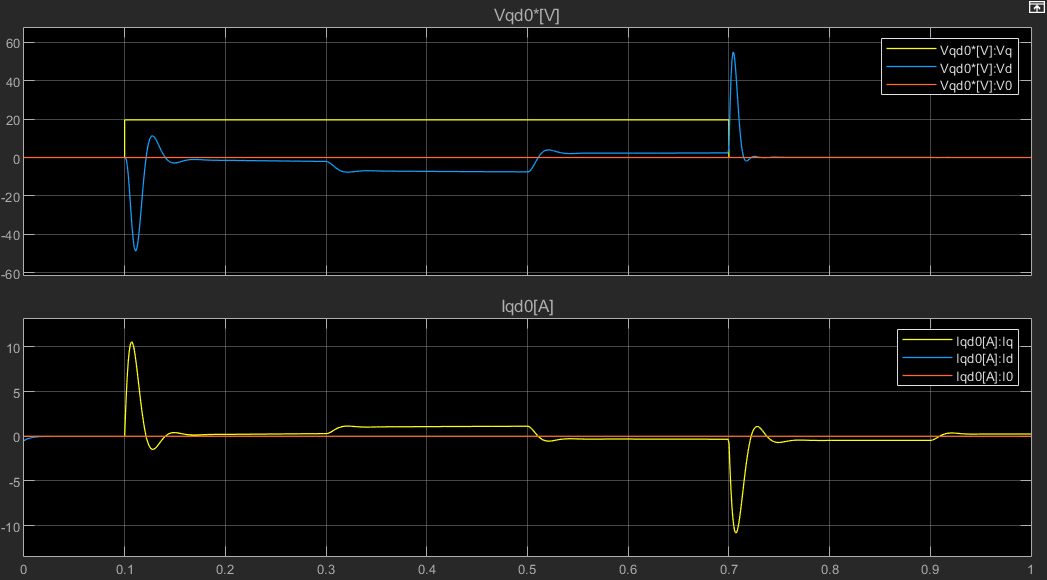
\includegraphics[width=0.95\textwidth]{Imagenes/ComparacionTensionesCorrientesVirtuales.png}
    \caption{Tensiones y corrientes en coordenadas virtuales.}
    \label{fig:ComparacionTensionesCorrientesVirtuales}
\end{figure}

El comportamiento de las consignas de tensiones convertidas a coordenadas reales abc se observa en la Figura~\ref{fig:SimulaciónTensionesCoordenadasReales} y detalladamente en la Figura~\ref{fig:TensionesRealesAcercamientoGlobalDT} con un acercamiento a $t = 0{.}1\,\text{s}$, donde se observa un comportamiento trifasico con un corto transitorio inicial y un sistema estable en valores de hasta 19.63V máximos. Se puede observar que este valor máximo, cuando el sistema se encuentra estable, se establece en 20.85V luego del primer escalón de la consigna de torque \(T_{ld}\) en el instante $t = 0{.}3\, \text{s}$, y en 19.73V a partir del instante $t = 0{.}5\, \text{s}$ en el segundo escalón de torque de valor negativo. 

\begin{figure}[H]
    \centering
    \begin{subfigure}[b]{0.45\textwidth}
        \centering
        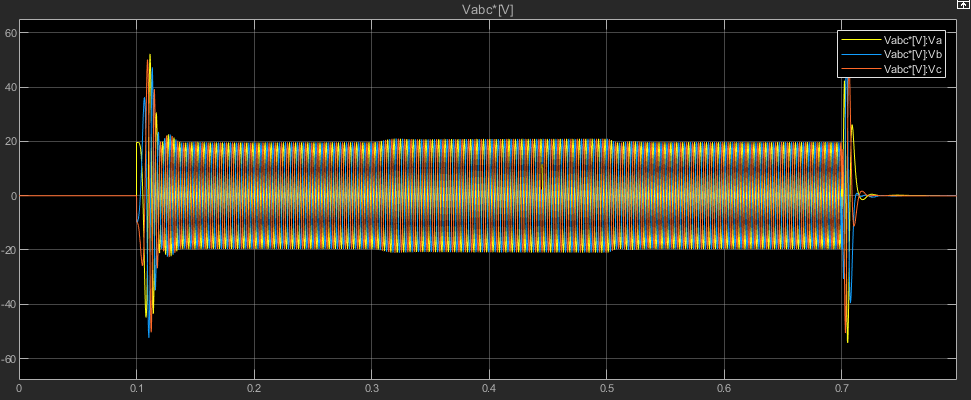
\includegraphics[width=\textwidth]{Imagenes/ConsignasTensionABC.png}
        \caption{Tensiones reales abc \(V_{abcs}\).}
        \label{fig:TensionesRealesGlobalDT}
    \end{subfigure}
    \hfill
    \begin{subfigure}[b]{0.45\textwidth}
        \centering
        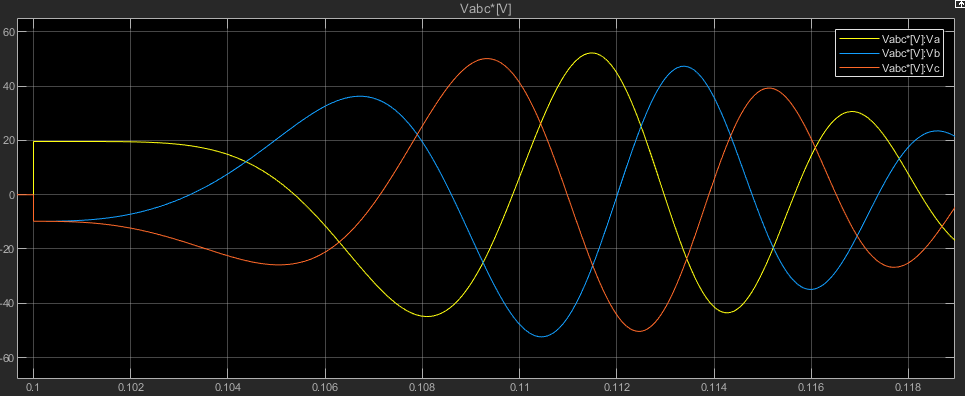
\includegraphics[width=\textwidth]{Imagenes/ConsignasTensionABCacercamiento.png}
        \caption{Acercamiento a $t = 0{.}1\,\text{s}$}
        \label{fig:TensionesRealesAcercamientoGlobalDT}
    \end{subfigure}
    \caption{Tensiones aplicadas en coordenadas reales.}
    \label{fig:SimulaciónTensionesCoordenadasReales}
\end{figure}
El comportamiento de las corrientes resultantes en coordenadas reales abc se observa en la Figura~\ref{fig:SimulaciónCorrientesCoordenadasReales} y detalladamente con un acercamiento al instante $t = 0{.}1\,\text{s}$ en la Figura~\ref{fig:CorrientesRealesAcercamientoGlobalDT}. Se observa inicialmente un transitorio en las corrientes que provocan picos máximos de hasta 10.86A en el caso de la corriente \(i_{bs}(t)\) (curva azul), y luego el comportamiento de las corrientes sigue una forma senoidal que se corresponde con el comportamiento de las tensiones. 

\begin{figure}[H]
    \centering
    \begin{subfigure}[b]{0.5\textwidth}
        \centering
        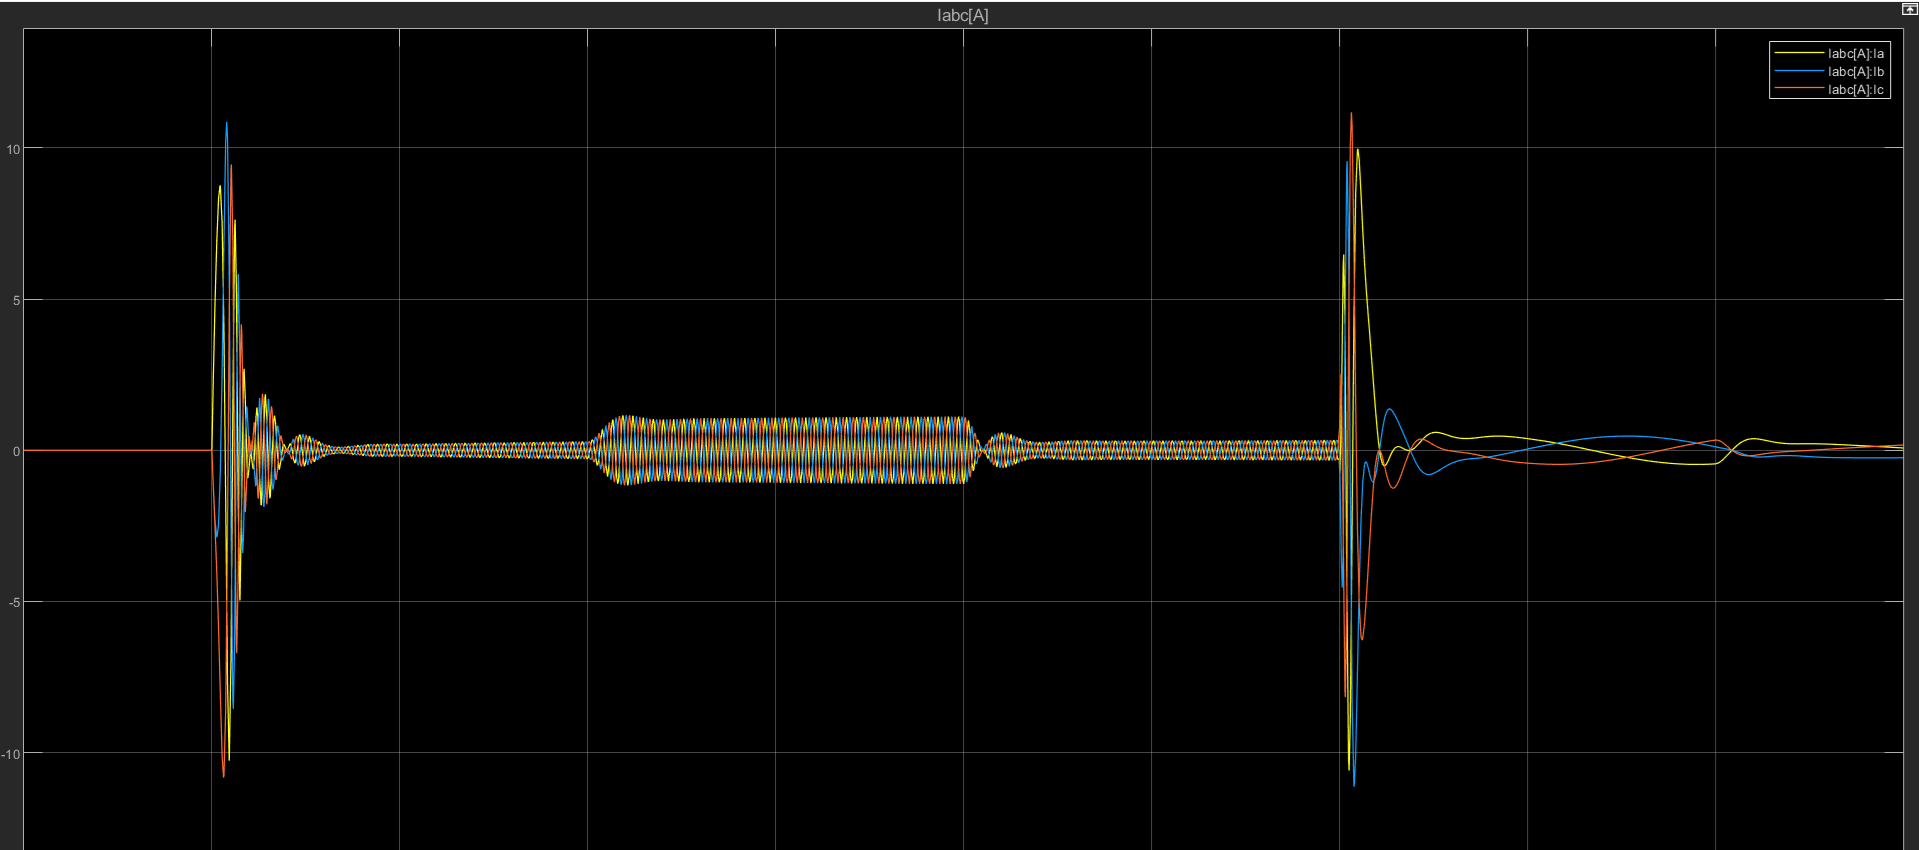
\includegraphics[width=\textwidth]{Imagenes/CorrientesABCSimulacion.png}
        \caption{Corrientes reales abc \(I_{abcs}\).}
        \label{fig:CorrientesRealesGlobalDT}
    \end{subfigure}
    \hfill
    \begin{subfigure}[b]{0.48\textwidth}
        \centering
        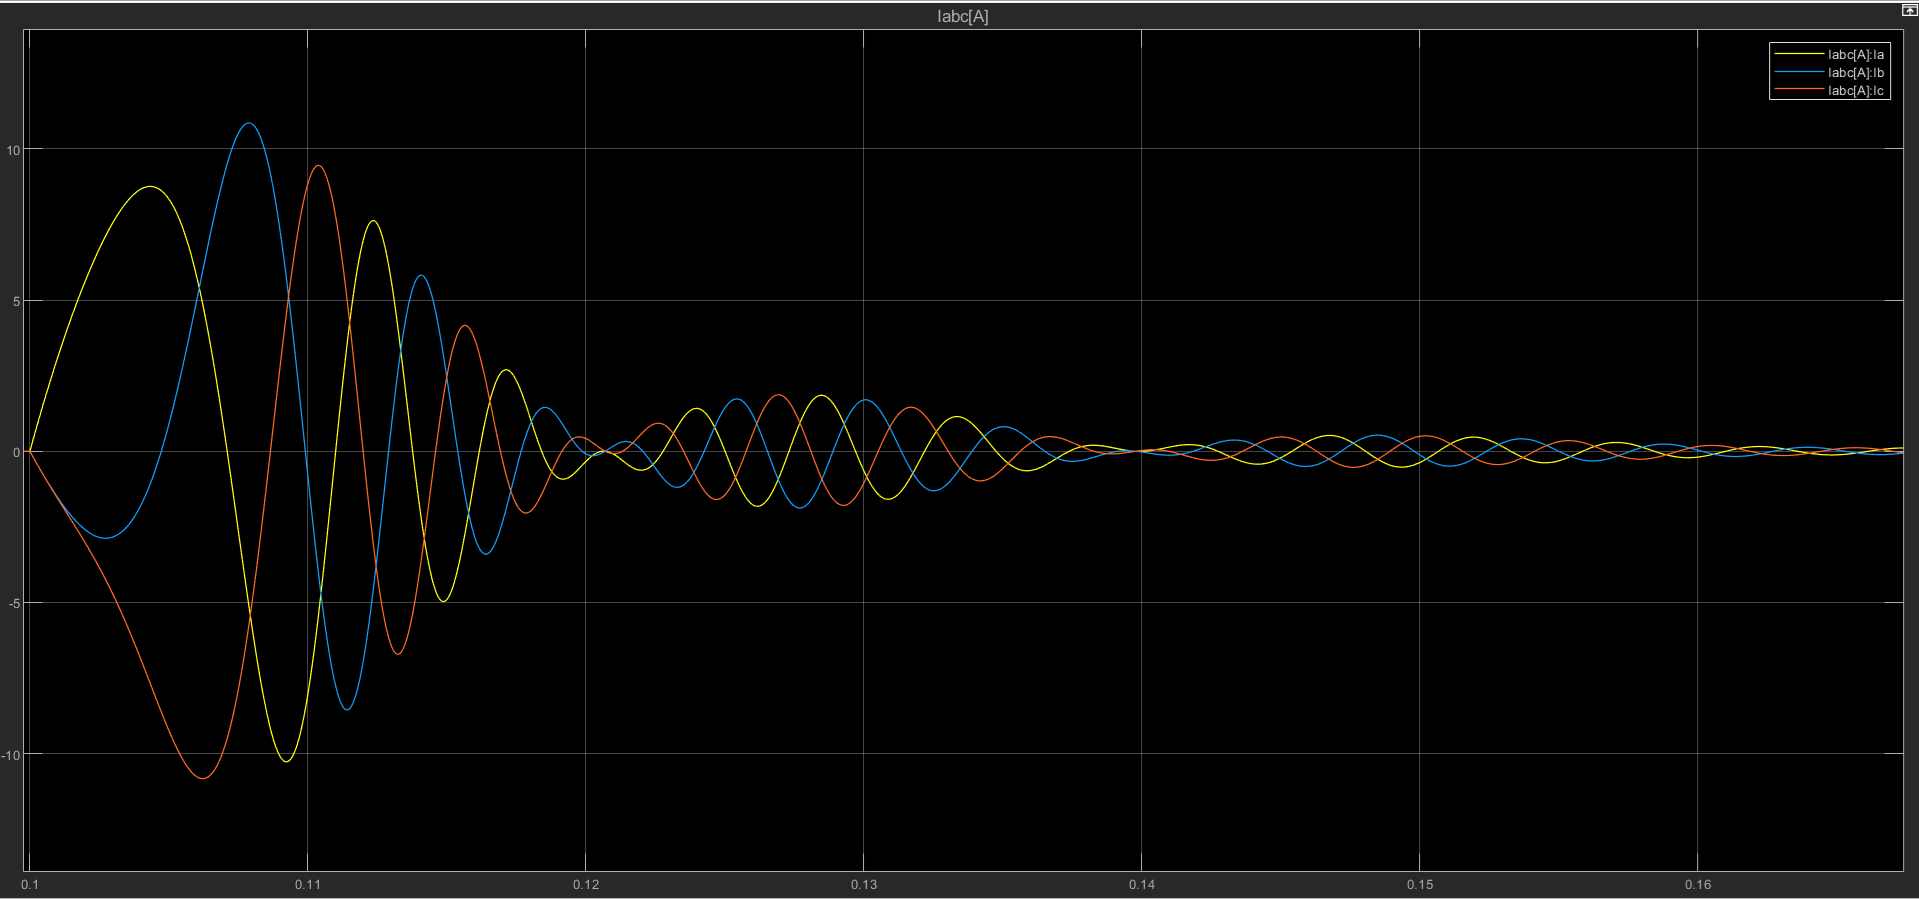
\includegraphics[width=\textwidth]{Imagenes/CorrientesABCacercamientoSimulacion.png}
        \caption{Acercamiento a $t = 0{.}1\,\text{s}$}
        \label{fig:CorrientesRealesAcercamientoGlobalDT}
    \end{subfigure}
    \caption{Corrientes resultantes en coordenadas reales.}
    \label{fig:SimulaciónCorrientesCoordenadasReales}
\end{figure}

En las figuras~\ref{fig:ComparativaVelocidadAngular} y~\ref{fig:ComparativaCorrientesVirtuales} se observan algunas comparaciones entre el modelo global NL y el sistema LTI aumentado. Se han comparado las curvas de velocidad angular y corrientes en coordenadas virtuales. La diferencia entre el sistema NL completo desacoplado con ley de control y el sistema LTI equivalente aumentado se debe a que el sistema LTI no considera las variaciones de Rs(t) con la temperatura, considerándola como una constante ``$R_s = R_{sREF} \approx 1.02\:\Omega\:(20\:^{\circ}\text{C})$''. Por lo tanto para el sistema NL, cuando la temperatura del estator es menor a Ts$<20^{\circ}$C la resistencia ``Rs$<1.02\:\Omega$'' será menor que la de referencia a 20$^{\circ}$C, generando así una mayor corriente en el sistema (Figura~\ref{fig:ComparativaCorrientesVirtuales}) y sus efectos consecuentes (el efecto contrario se produce cuando Ts$>20^{\circ}$C).

\begin{figure}[H]
    \centering
    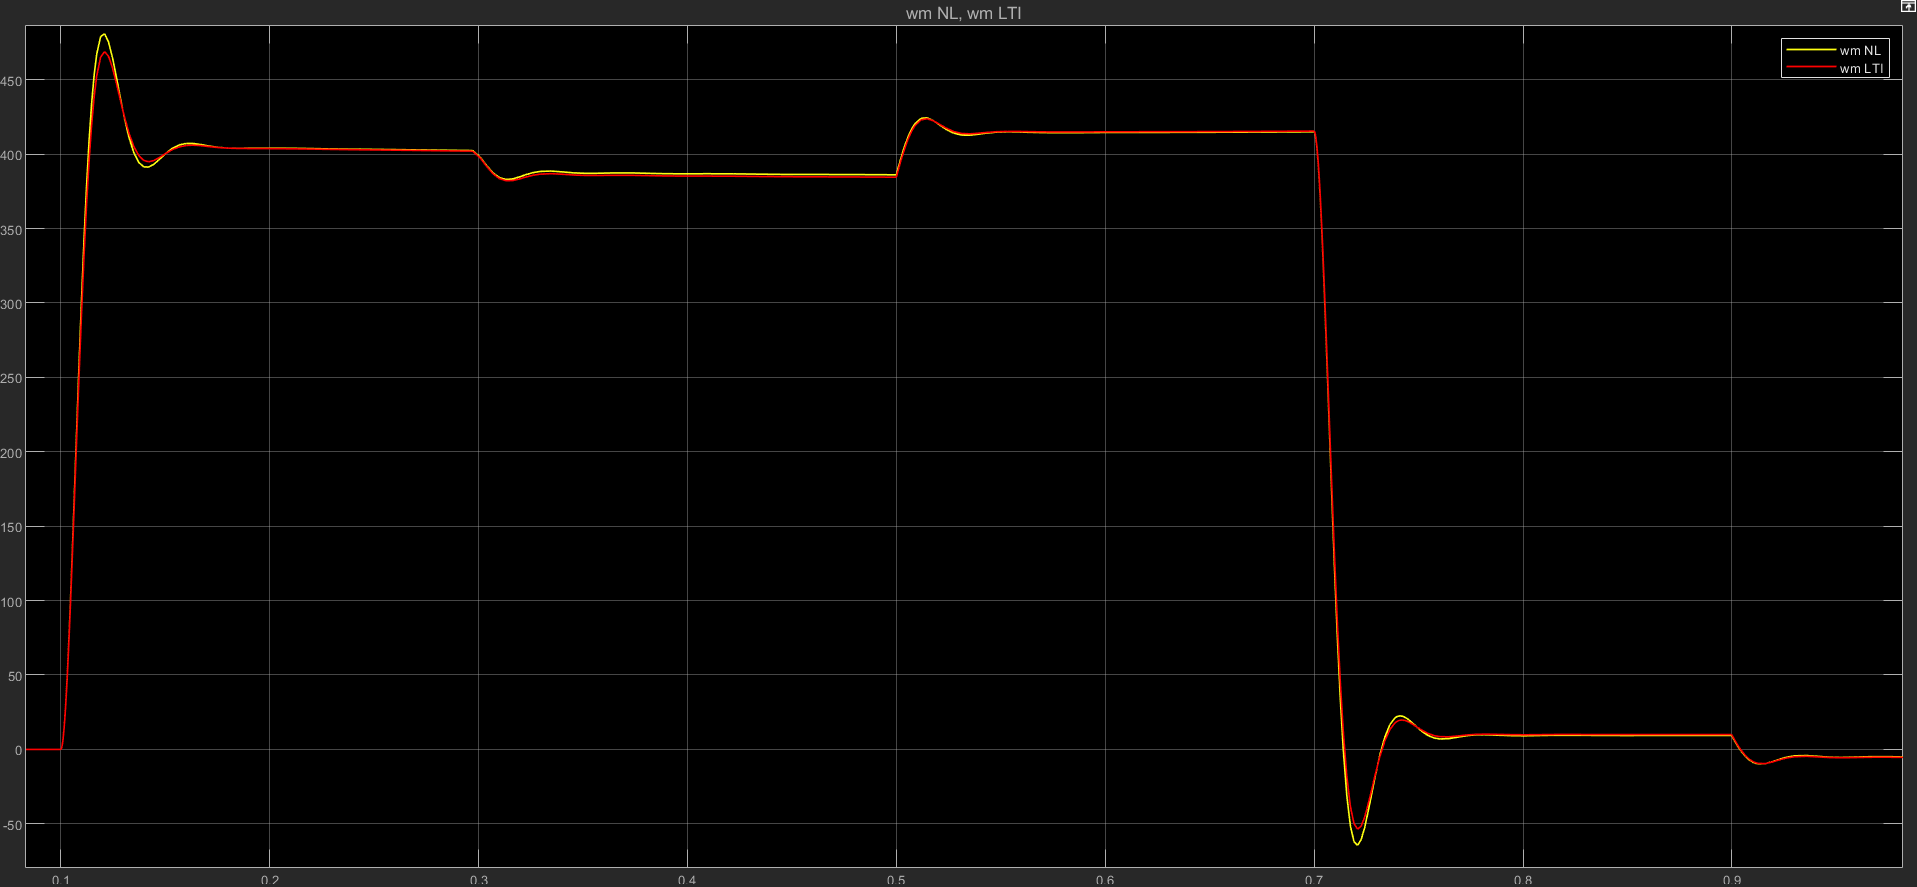
\includegraphics[width=1\textwidth]{Imagenes/ComparativaVelocidadAngular.png}
    \caption{Comparación de la velocidad angular entre el sistema NL y el sistema LTI aumentado. Amarillo: sistema NL - Rojo: sistema LTI aumentado.}
    \label{fig:ComparativaVelocidadAngular}
\end{figure}


\begin{figure}[H]
    \centering
    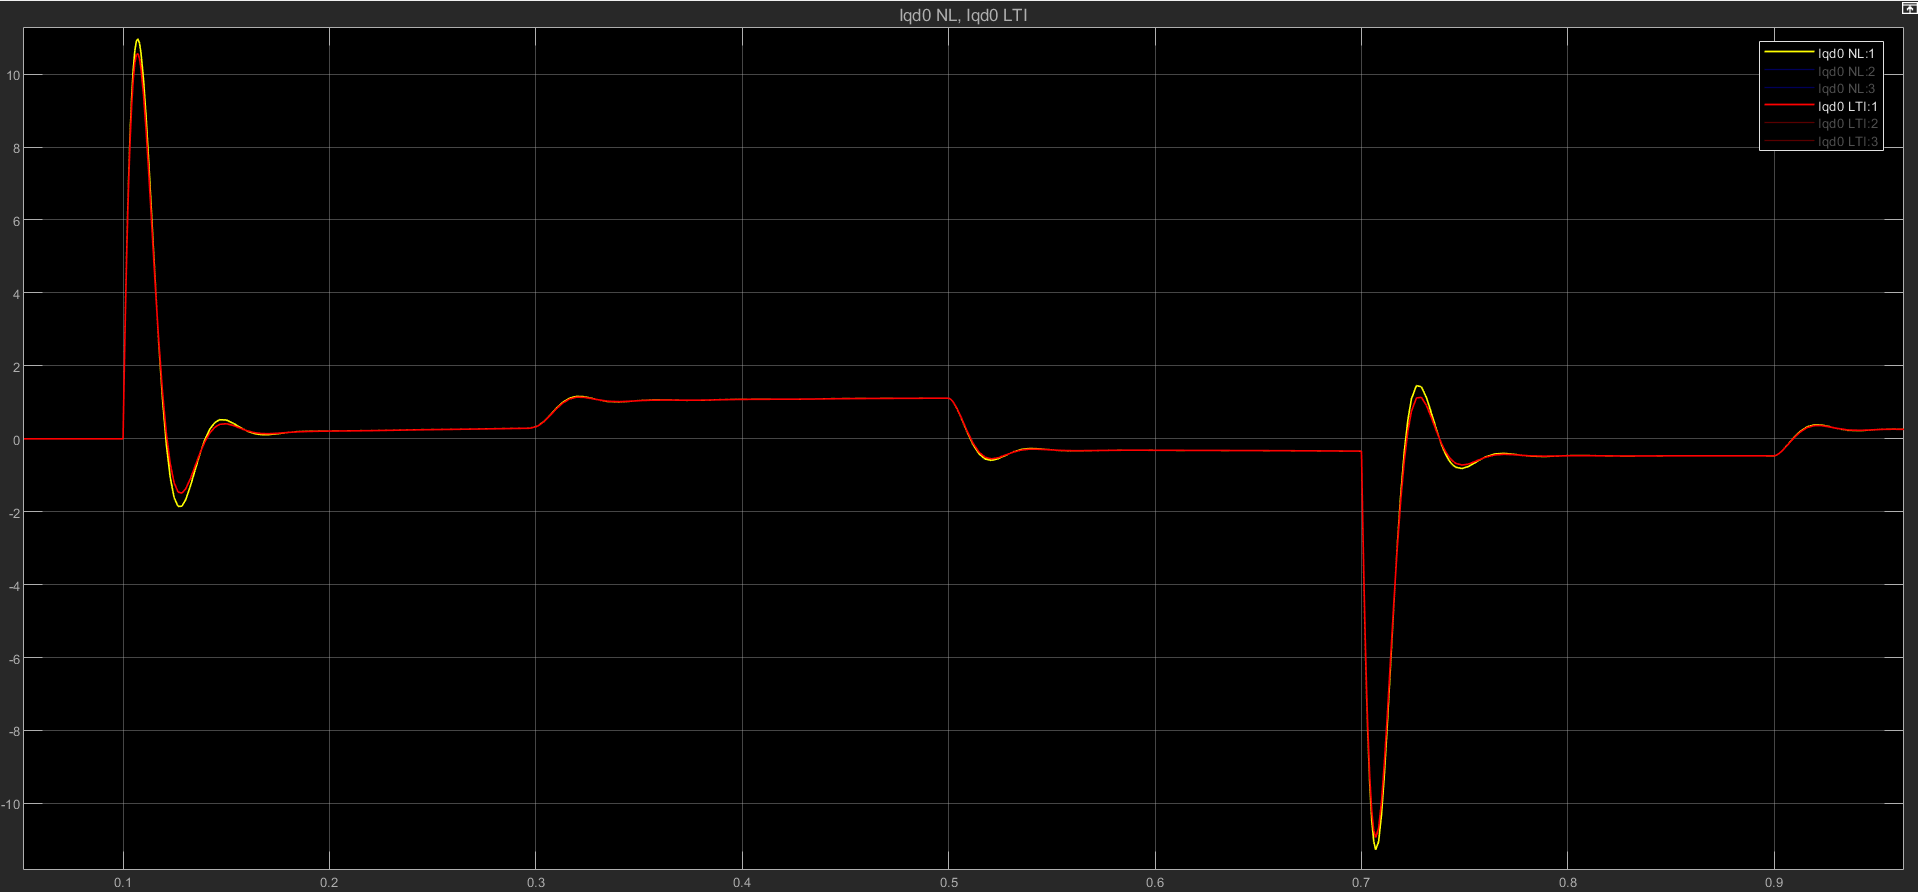
\includegraphics[width=1\textwidth]{Imagenes/ComparativaCorrientesVirtuales.png}
    \caption{Comparación de las corrientes virtuales entre el sistema NL y el sistema LTI aumentado. Amarillo: sistema NL - Rojo: sistema LTI aumentado.}
    \label{fig:ComparativaCorrientesVirtuales}
\end{figure}


\newpage
La curva paramétrica $\omega_m$-$T_m$ mostrada en la Figura~\ref{fig:CurvaParametricaTorquevsVelocidad} representa el comportamiento dinámico del sistema, construida a partir de los pares ordenados $(\omega_m(t),T_m(t))$ correspondientes a la velocidad angular del eje mecánico y el torque electromagnético, respectivamente, para cada instante $t$ de simulación. En esta representación se identifican 6 puntos agudos que corresponden a estados de equilibrio del sistema dinámico bajo las condiciones de entrada especificadas. La curva se puede dividir en 5 segmentos, cada uno representado con un color diferente, que conectan pares sucesivos de puntos de equilibrio. Estos segmentos constituyen las trayectorias de transición del sistema, es decir, los conjuntos de puntos que describen la evolución temporal del sistema cuando se desplaza de un estado de equilibrio a otro. Esta visualización permite apreciar tanto los estados estacionarios como la dinámica transitoria del sistema en el espacio de estados $\omega_m$-$T_m$.
\begin{figure}[H]
    \centering
    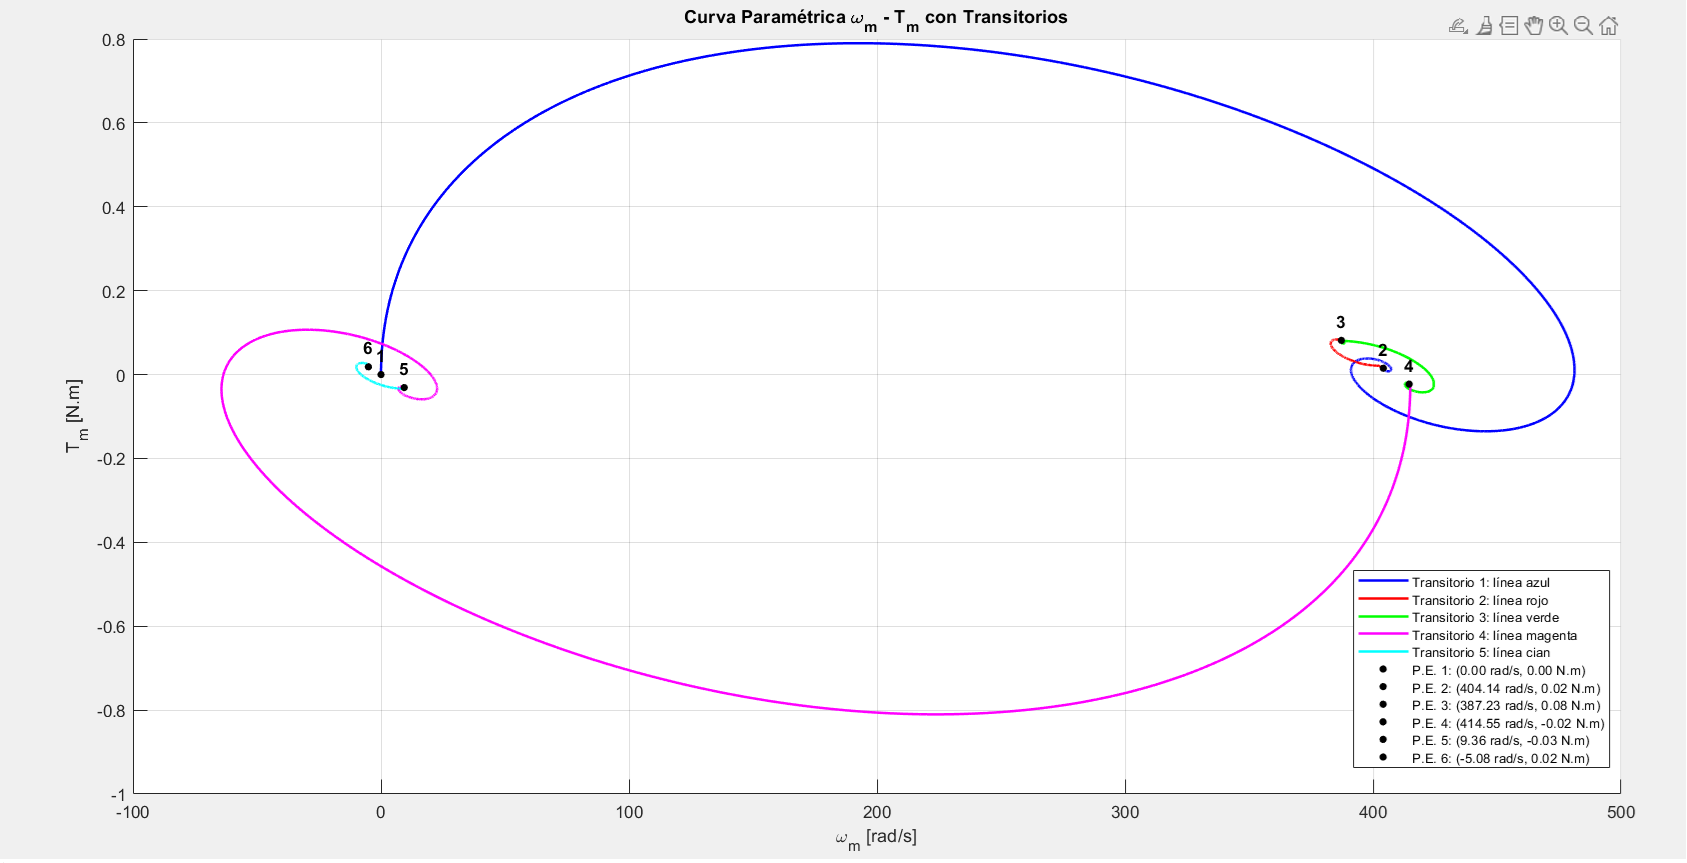
\includegraphics[width=0.8\textwidth]{Imagenes/CurvaParametricaWm-Tm.png}
    \caption{Curvas paramétricas de Torque vs Velocidad.}
    \label{fig:CurvaParametricaTorquevsVelocidad}
\end{figure}


\subsection*{Cálculo del Ángulo de Carga \(\delta(t)\)}

El ángulo de carga \(\delta(t)\), también conocido como el \textit{ángulo de defasaje electromagnético del rotor}, representa el desplazamiento angular entre la coordenada eléctrica sincrónica \(\theta_{ev}\) y la posición angular del rotor en coordenadas eléctricas \(\theta_r\). Se define como:

\begin{equation}
    \delta(t) \equiv \theta_{ev}(t) - \theta_r(t) = \int_0^t [\omega_e(\xi) - \omega_r(\xi)] d\xi + [\theta_{ev}(0) - \theta_r(0)]
\end{equation}

donde:
\begin{itemize}
    \item \(\omega_e\) es la velocidad angular de la referencia sincrónica.
    \item \(\omega_r\) es la velocidad angular del rotor.
    \item \(\theta_{ev}(0)\) y \(\theta_r(0)\) son las condiciones iniciales de los ángulos.
\end{itemize}

\subsubsection*{Cálculo de la Coordenada Eléctrica Sincrónica \(\theta_{ev}\)}

Para obtener \(\theta_{ev}(t)\), primero se aplicó la transformación de Clarke a las tensiones trifásicas del estator \((V_a, V_b, V_c)\), obteniendo las componentes en coordenadas \(\alpha \beta\):

\begin{equation}
    V_{\alpha} = \frac{2}{3} \left( V_a - \frac{1}{2} V_b - \frac{1}{2} V_c \right),
\end{equation}

\begin{equation}
    V_{\beta} = \frac{\sqrt{3}}{3} (V_b - V_c).
\end{equation}

Luego, la fase instantánea \(\theta_{ev}\) de la señal se calculó con la función \(\operatorname{atan2}\):

\begin{equation}
    \theta_{ev} = \operatorname{atan2}(V_{\beta}, V_{\alpha}).
\end{equation}

Dado que la función \(\operatorname{atan2}\) solo devuelve valores en el intervalo \([- \pi, \pi]\), fue necesario corregir la fase para evitar discontinuidades en la señal al cruzar estos límites. Para ello, se implementó un bloque \texttt{MATLAB Function} en Simulink que ajusta \(\theta_{ev}\) considerando los ciclos completos de \(2\pi\).

\subsubsection*{Implementación en Simulink}

En la Figura~\ref{fig:BloquesAnguloCarga} se presenta el diagrama en bloques utilizado en Simulink para la obtención del ángulo de carga \(\delta(t)\). Se puede observar la transformación de Clarke aplicada a las tensiones trifásicas, la obtención de \(\theta_{ev}\) mediante la función \(\operatorname{atan2}\), la corrección de fase y el cálculo de \(\delta(t)\) restando \(\theta_r\), que se obtiene multiplicando la posición angular del rotor mecánico \(\theta_m\) por el número de pares de polos \(P\).

\begin{figure}[H]
    \centering
    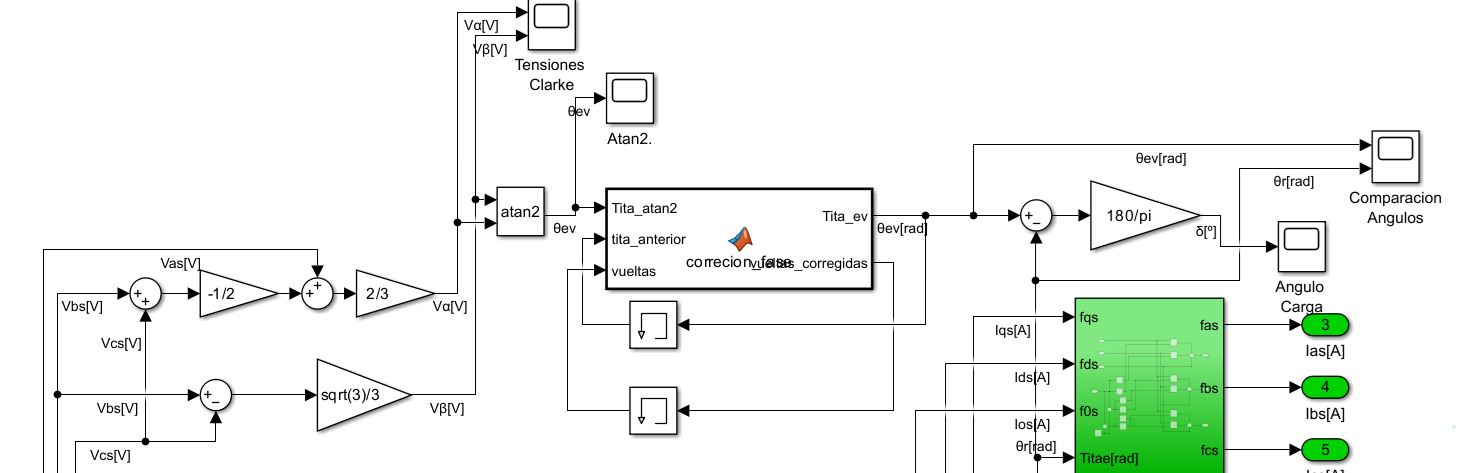
\includegraphics[width=0.8\textwidth]{Imagenes/BloquesAnguloCarga.png}
    \caption{Diagrama en bloques en Simulink para el cálculo del ángulo de carga \(\delta\).}
    \label{fig:BloquesAnguloCarga}
\end{figure}

\subsubsection*{Resultados de la Simulación}

En la Figura~\ref{fig:AnguloCargaSimulacionDT} se presenta la evolución temporal del ángulo de carga \(\delta(t)\). Se observa que la corrección de fase implementada en el bloque \texttt{MATLAB Function} permite obtener una señal continua y sin discontinuidades abruptas al cruzar múltiplos de \(\pi\).

\begin{figure}[H]
    \centering
    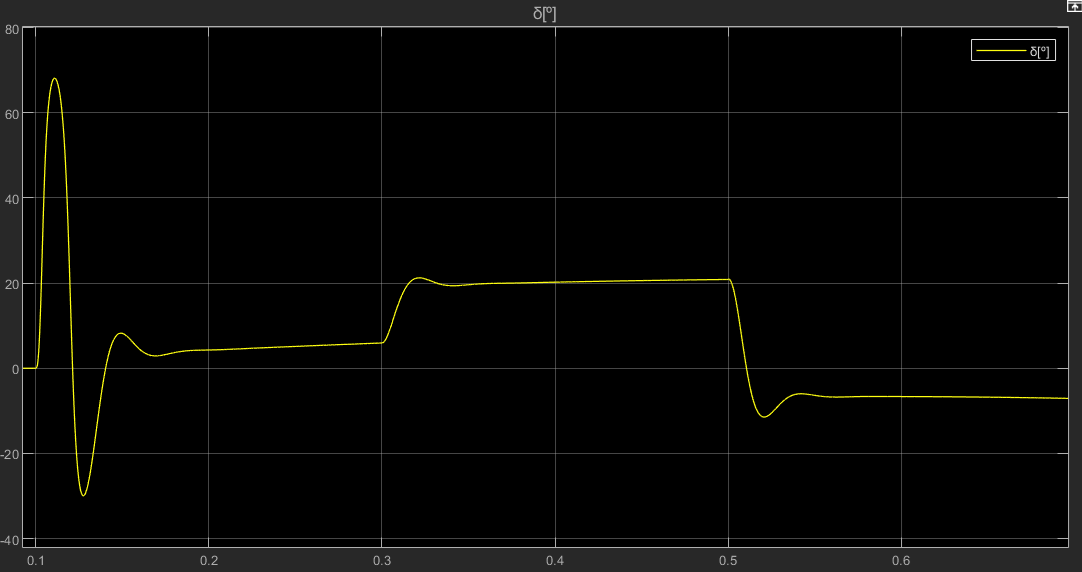
\includegraphics[width=0.7\textwidth]{Imagenes/AnguloCargaSimulacionDT.png}
    \caption{Respuesta temporal del ángulo de carga \(\delta(t)\).}
    \label{fig:AnguloCargaSimulacionDT}
\end{figure}

Estos resultados permiten analizar el comportamiento de la máquina eléctrica en términos de su sincronización con el campo magnético del estator, permitiendo evaluar su operación en diferentes condiciones de carga y control.



\subsubsection{Determinación de velocidad y corriente final de establecimiento}

En la Tabla~\ref{table:parametros_sistema} se observan los valores de velocidad y corriente final de establecimiento luego de cada transitorio, tiempos de crecimiento (10\% al 90\% de intervalo entre valores inicial y final), tiempo de establecimiento ($\pm$1\%) y sobrepico. 

\textbf{¿Qué influencia relativa tienen cada una de las dos acciones externas? ¿A qué se debe?} Al aplicar una tensión \(V^r_{qs}\), el eje mecánico de la máquina eléctrica comienza a moverse hasta alcanzar la velocidad angular $\omega_m$ de equilibrio. Se observa que ante el primer escalón \(T_{ld}\) la velocidad angular disminuye, esto se debe a que la perturbación se opone al torque electromagnético \(T_m\) (considerando una convención de signos para el torque de perturbación tal que el signo + implica una dirección contraria a la dirección de movimiento), reduciendo el torque resultante total sobre el eje mecánico. En el instante $t = 0.5\, \text{s}$ ocurre lo opuesto, el escalón \(T_{ld}\) ahora tiene valor negativo lo que significa que refuerza al torque electromagnético, aumentando el torque resultante sobre el eje de la máquina, aumentando la velocidad $\omega_m$. Al cesar el escalón de tensión \(V^r_{qs}\) en el instante $t = 0.7\, \text{s}$, el torque resultante tiende a ser 0 excepto por el escalón negativo de \(T_{ld}\) que dura hasta el instante $t = 0.9\, \text{s}$, lo que provoca que aún el eje mecánico de la máquina gire a una velocidad $\omega_m$. Cuando el escalón negativo de \(T_{ld}\) cesa, la velocidad angular $\omega_m$ del eje mecánico de la máquina decae a 0.

\begin{table}[htbp]
   \centering
   \begin{tabular}{|c|c|c|c|c|c|}
       \hline
       \multicolumn{6}{|c|}{Parámetros del sistema} \\
       \hline
       & $V_q = 19.596V$ & $T_{ld} = 6.28\text{N.m}$ & $T_{ld} = -6.28\text{N.m}$ & $V_q = 0V$ & $T_{ld} = 0\text{N.m}$ \\
       & $t = 0.1\text{s}$ & $t = 0.3\text{s}$ & $t = 0.5\text{s}$ & $t = 0.7\text{s}$ & $t = 0.9\text{s}$ \\
       \hline
       $\omega_m$ Final [rad/s] & 403.90 & 387.1 & 414.50 & 9.50 & -5.35 \\
       \hline
       Tiempo de levantamiento $t_r$ [s] & 0.013 & 0.007 & 0.006 & 0.014 & 0.0071 \\
       \hline
       Tiempo de asentamiento $t_s$ [s] & 0.083 & 0.014 & 0.022 & 0.076 & 0.049 \\
       \hline
       Sobrepico [rad/s] & 77.27 & -7.161 & 4.046 & -55.442 & -2.5673 \\
       \hline
       \hline
       $i_q$ Final [A] & 0.2094 & 1.063 & -0.3155 & -0.468 & 0.2522 \\
       \hline
       Tiempo de levantamiento $t_r$ [s] & 0.000623 & 0.0145 & 0.0134 & 0.00039 & 0.004200 \\
       \hline
       Tiempo de asentamiento $t_s$ [s] & 0.094 & 0.055 & 0.0052 & 0.083828 & 0.0052 \\
       \hline
       Sobrepico [A] & 10.76 & 0.100 & -0.22 & -10.782 & 0.1314 \\
       \hline
   \end{tabular}
   \caption{Parámetros característicos de la respuesta dinámica del sistema ante variaciones de tensión y torque de carga}
   \label{table:parametros_sistema}
\end{table}
\newpage
\subsubsection{Comportamiento de \(i^r_{ds}(t)\) para \(i^r_{ds}(0) \neq 0\) y comparación entre modelos NL completo vs LTI aumentado}

Ahora se observará el comportamiento de las corrientes en coordenadas virtuales \(i^r_{qd0s}\) frente a una condición inicial \(i^r_{ds}(0) = \pm0{.}5A\). Tanto en la figura~\ref{fig:CorrientesVirtualesId0.5A} como en la figura~\ref{fig:CorrientesVirtualesId-0.5A} se observa que no hay cambios en el comportamiento de las corrientes respecto de lo que se observó en la Figura~\ref{fig:ComparacionTensionesCorrientesVirtuales} con condición inicial nula \(i^r_{ds}(0) = 0\). También se observa el rápido decaimiento exponencial de la corriente \(i^r_{ds}(t)\) en las figuras~\ref{fig:DecaimientoCorrienteId0.5A} y~\ref{fig:DecaimientoCorrienteId-0.5A}. 


\begin{figure}[H]
    \centering
    % Primera fila con las subfiguras (a) y (b)
    \begin{subfigure}[b]{0.42\textwidth}
        \centering
        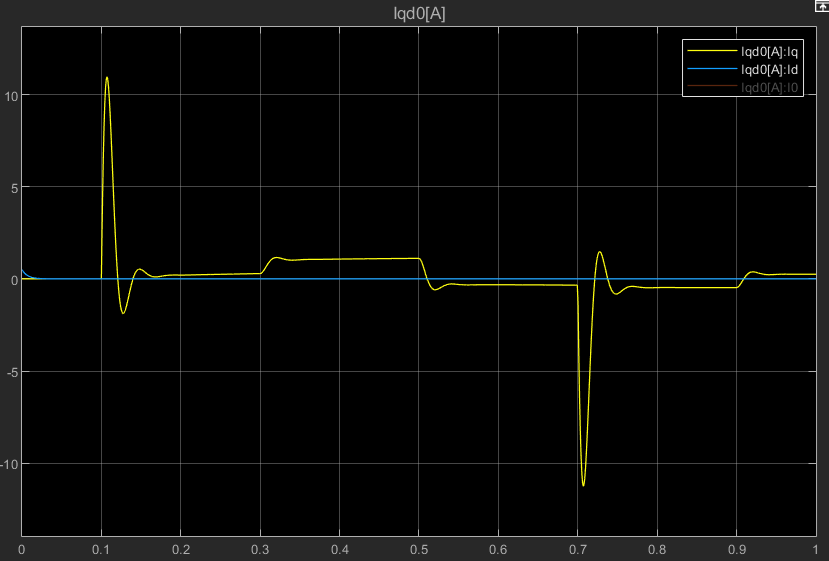
\includegraphics[width=\textwidth]{Imagenes/CorrientesVirtualesId0,5A.png}
        \caption{Corrientes virtuales \(i^r_{qd0s}\).}
        \label{fig:CorrientesVirtualesId0.5A}
    \end{subfigure}
    \hfill
    \begin{subfigure}[b]{0.4\textwidth}
        \centering
        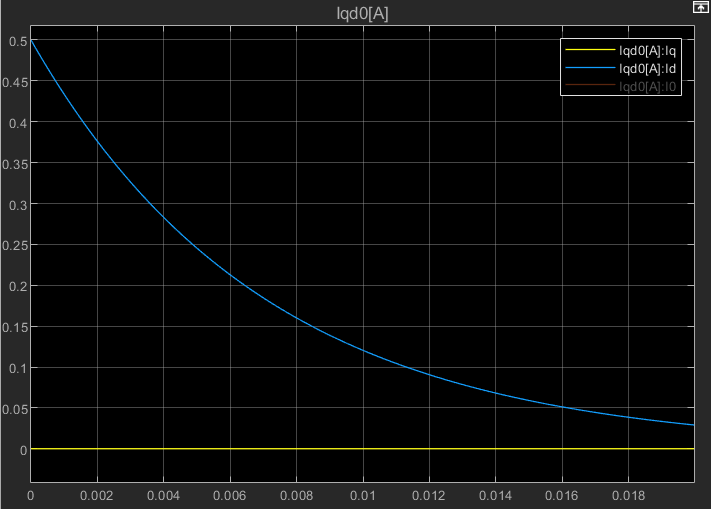
\includegraphics[width=\textwidth]{Imagenes/DecaimientoCorrienteId0,5A.png}
        \caption{Decaimiento exponencial de la corriente \(i^r_{ds}\).}
        \label{fig:DecaimientoCorrienteId0.5A}
    \end{subfigure}
    
    \vspace{0.5cm} % Espacio vertical entre las filas

    % Segunda fila con las subfiguras (c) y (d)
    \begin{subfigure}[b]{0.42\textwidth}
        \centering
        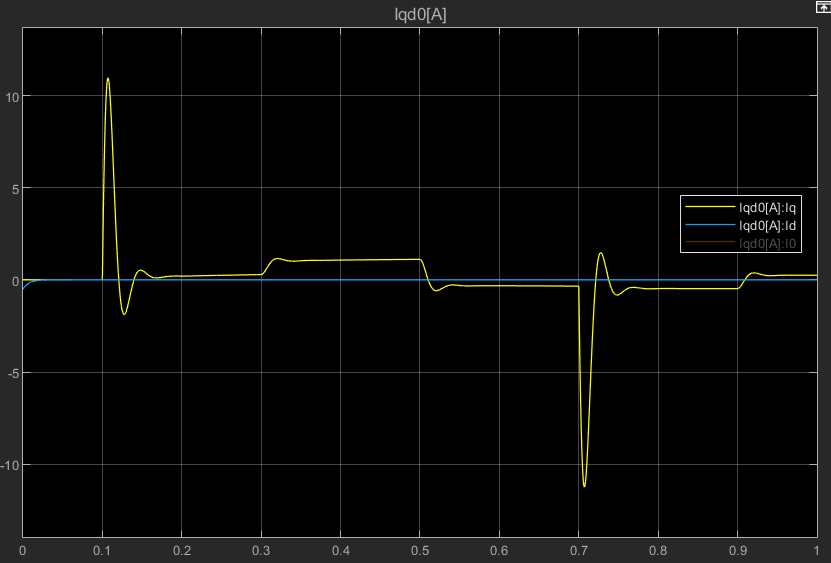
\includegraphics[width=\textwidth]{Imagenes/CorrientesVirtualesId-0,5A.png}
        \caption{Corrientes virtuales \(i^r_{qd0s}\).}
        \label{fig:CorrientesVirtualesId-0.5A}
    \end{subfigure}
    \hfill
    \begin{subfigure}[b]{0.4\textwidth}
        \centering
        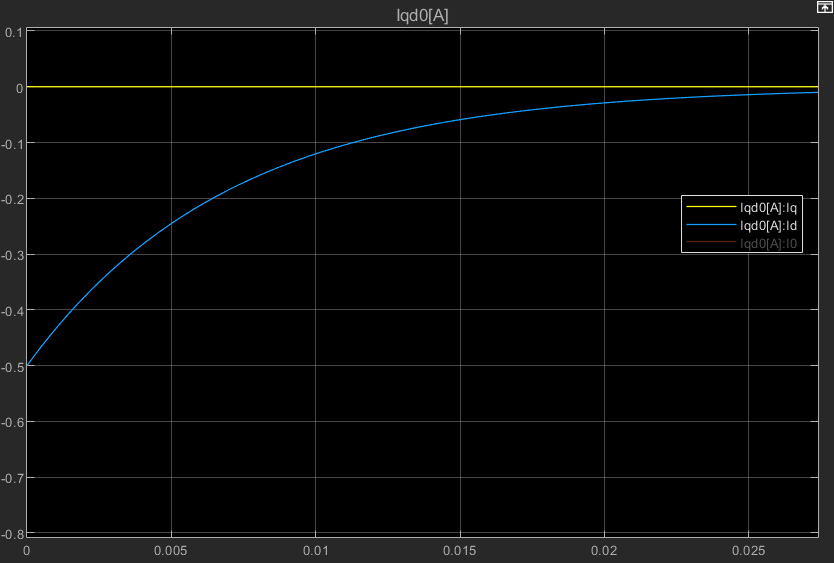
\includegraphics[width=\textwidth]{Imagenes/DecaimientoCorrienteId-0,5A.png}
        \caption{Decaimiento exponencial de la corriente \(i^r_{ds}\).}
        \label{fig:DecaimientoCorrienteId-0.5A}
    \end{subfigure}

    \caption{Corrientes virtuales \(i^r_{qd0s}\) en el modelo NL completo dadas dos condiciones iniciales: \(i^r_{ds}(0) = 0.5A\) (subfiguras (a) y (b)) y \(i^r_{ds}(0) = -0.5A\) (subfiguras (c) y (d)).}
    \label{fig:CorrientesVirtualesCondicionId}
\end{figure}

Finalmente se comparan los resultados con el modelo LTI equivalente aumentado de la Figura~\ref{fig:diagrama_sistema_LTI_aumentado} (sección~\ref{sec:modelo_LTI}), y se observan comportamientos prácticamente idénticos en ambos modelos. En las figuras~\ref{fig:CorrientesVirtualesId0.5ALTIaumentado} y~\ref{fig:CorrientesVirtualesId-0.5ALTIaumentado} se ilustran las respuestas de las corrientes en coordenadas virtuales frente a las condiciones iniciales \(i^r_{ds}(0) = 0.5A\) y \(i^r_{ds}(0) = -0.5A\) y en las figuras~\ref{fig:DecaimientoCorrienteId0.5ALTIaumentado} y~\ref{fig:DecaimientoCorrienteId-0.5ALTIaumentado} los decaimientos exponenciales de la corriente \(i^r_{ds}(t)\) correspondientes. La similitud de las respuestas de corrientes en ambos modelos (NL completo desacoplado con Ley de Control NL vs LTI equivalente aumentado),
confirma la efectividad del desacople realizado entre ejes de corriente \textbf{q} y \textbf{d} con la \textbf{Ley de Control complementaria mínima en el eje q} del ítem 2.c.VI de la consigna del Trabajo Integrador.

\begin{figure}[H]
    \centering
    % Primera fila con las subfiguras (a) y (b)
    \begin{subfigure}[b]{0.42\textwidth}
        \centering
        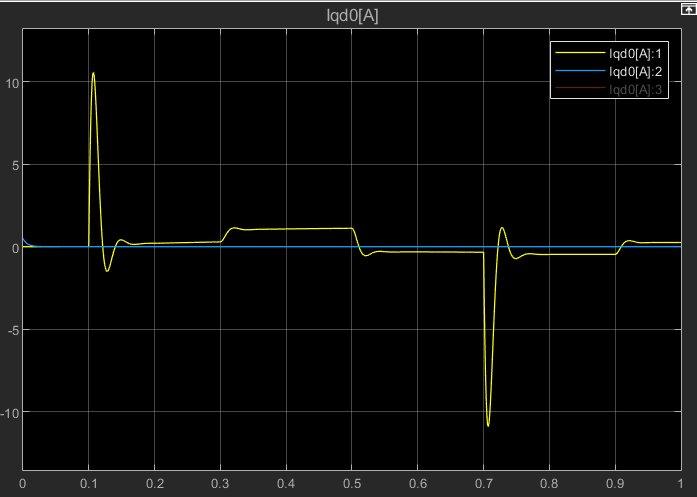
\includegraphics[width=\textwidth]{Imagenes/CorrientesVirtuales0,5ALTIaumentado.png}
        \caption{Corrientes virtuales \(i^r_{qd0s}\).}
        \label{fig:CorrientesVirtualesId0.5ALTIaumentado}
    \end{subfigure}
    \hfill
    \begin{subfigure}[b]{0.4\textwidth}
        \centering
        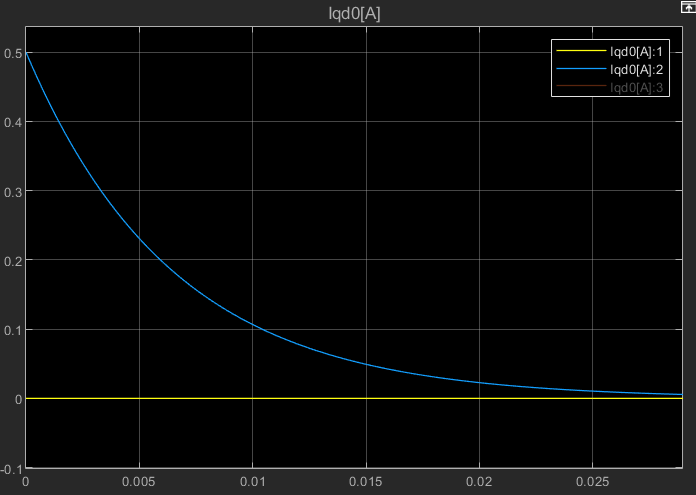
\includegraphics[width=\textwidth]{Imagenes/DecaimientoCorrienteId0,5ALTIaumentado.png}
        \caption{Decaimiento exponencial de la corriente \(i^r_{ds}\).}
        \label{fig:DecaimientoCorrienteId0.5ALTIaumentado}
    \end{subfigure}
    
    \vspace{0.5cm} % Espacio vertical entre las filas

    % Segunda fila con las subfiguras (c) y (d)
    \begin{subfigure}[b]{0.42\textwidth}
        \centering
        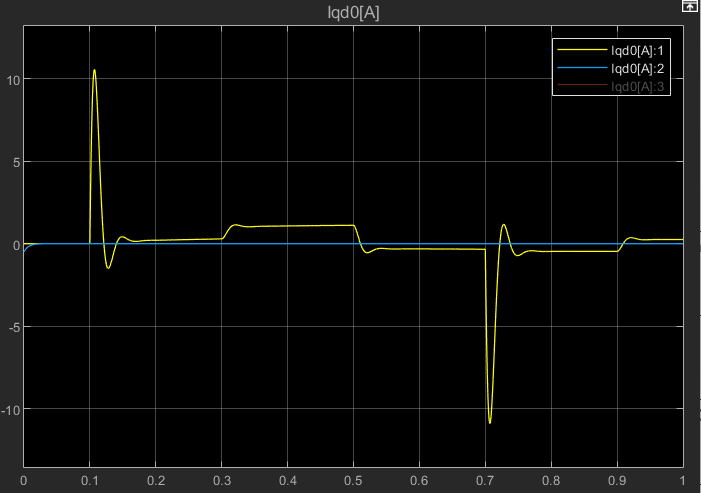
\includegraphics[width=\textwidth]{Imagenes/CorrientesVirtuales-0,5ALTIaumentado.png}
        \caption{Corrientes virtuales \(i^r_{qd0s}\).}
        \label{fig:CorrientesVirtualesId-0.5ALTIaumentado}
    \end{subfigure}
    \hfill
    \begin{subfigure}[b]{0.4\textwidth}
        \centering
        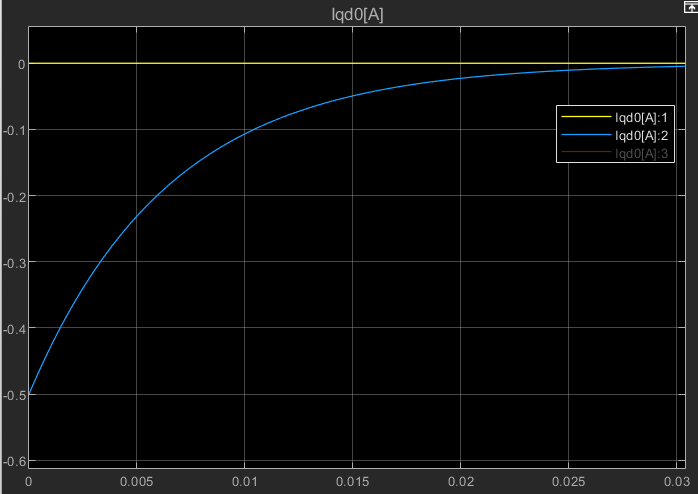
\includegraphics[width=\textwidth]{Imagenes/DecaimientoCorrienteId-0,5ALTIaumentado.png}
        \caption{Decaimiento exponencial de la corriente \(i^r_{ds}\).}
        \label{fig:DecaimientoCorrienteId-0.5ALTIaumentado}
    \end{subfigure}

    \caption{Corrientes virtuales \(i^r_{qd0s}\) en el modelo LTI equivalente aumentado dadas dos condiciones iniciales: \(i^r_{ds}(0) = 0.5A\) (subfiguras (a) y (b)) y \(i^r_{ds}(0) = -0.5A\) (subfiguras (c) y (d)).}
    \label{fig:CorrientesVirtualesCondicionIdLTIAumentado}
\end{figure}
\subsubsection{Comportamiento de los modelos con una consigna de tensión en el eje d, \(v^{r*}_{ds}(t) \equiv V^r_{qs nom}/10\)}

Se agrega una consigna de tensión en el eje d, \(v^{r*}_{ds}(t) \equiv V^r_{qs nom}/10 = \pm 1{.}9596 V_{cc}\) en \(t_{step1} = 0{.}5\, s\), sumada a la restricción o \textbf{Ley de Control mínima en el eje d}. 
Se observa que para una tensión $V_d(t)=1.9695V$ se comprueba el efecto de reforzamiento de campo (Field forcing), en donde el Torque electromagnético tiene sobreimpulsos mayores y la velocidad angular de establecimiento es menor. Por otro lado, para $V_{ds}(t)=-1.9695V$ se comprueba el efecto de debilitamiento de campo (Field weakening), donde se observan sobreimpulsos menores en el Torque electromagnético y una velocidad angular de establecimiento mayor respecto al sistema estándar con $V_{ds}(t)=0$. Se obtuvieron los siguientes resultados de las curvas de velocidad (Figura~\ref{fig:VelocidadAngular_ConsignasTensionVds}) y torque (Figura~\ref{fig:TorqueElectromagnetico_ConsignasTensionVds}).

\begin{figure}[H]
    \centering
    \begin{subfigure}[b]{0.5\textwidth}
        \centering
        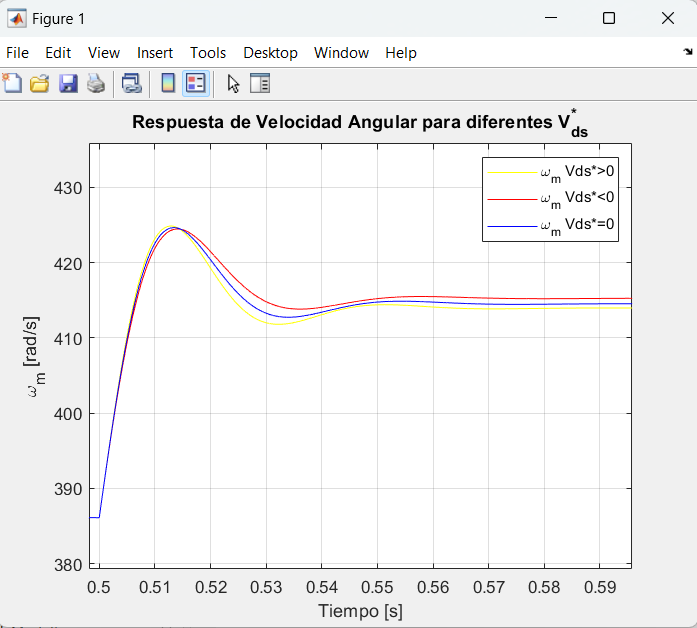
\includegraphics[width=\textwidth]{Imagenes/VelocidadAngular_ConsignasTensionVds.png}
        \caption{Velocidad angular para consignas de tensión \(v^r_{ds}(t) \pm 1{.}9695V\) y \(v^r_{ds}(t) = 0V\).}
        \label{fig:VelocidadAngular_ConsignasTensionVds}
    \end{subfigure}
    \hfill
    \begin{subfigure}[b]{0.48\textwidth}
        \centering
        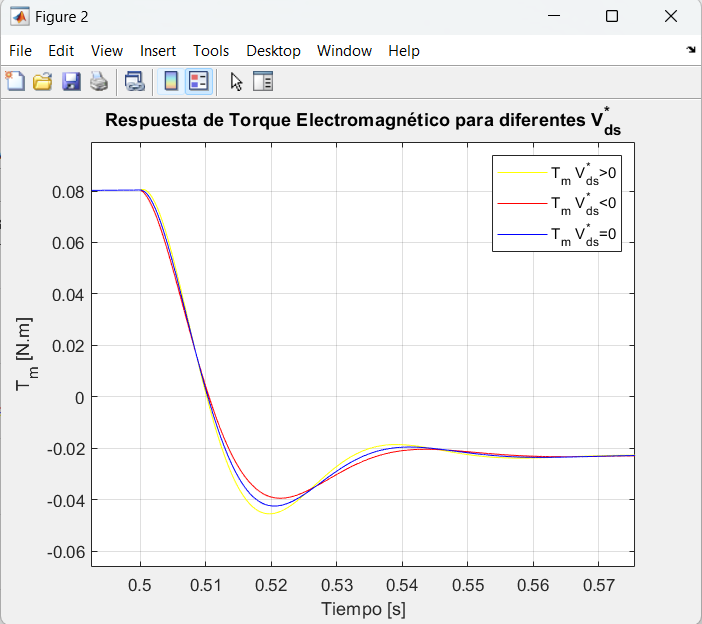
\includegraphics[width=\textwidth]{Imagenes/TorqueElectromagnetico_ConsignasTensionVds.png}
        \caption{Torque Electromagnético para consignas de tensión \(v^r_{ds}(t) \pm 1{.}9695V\) y \(v^r_{ds}(t) = 0V\).}
        \label{fig:TorqueElectromagnetico_ConsignasTensionVds}
    \end{subfigure}
    \caption{Comportamiento del modelo NL completo con consignas de tensión en el eje d.}
    \label{fig:ModeloNLcompletoConsignasTensionVds}
\end{figure}



\section{Diseño, Análisis y Simulación con Controlador de Movimiento}

\subsection{Modulador de Torque Equivalente}

En esta sección se desarrolla el modulador de torque equivalente que actuará como el lazo interno de control vectorial de corriente/torque. Este modulador recibe como consigna una referencia de torque \((T_m^*(t))\) y entrega las tensiones necesarias en coordenadas \((q,d,0)\) del estator, las cuales luego se transforman a coordenadas \((a,b,c)\) para alimentar el inversor trifásico. El objetivo principal es lograr un lazo interno rápido y desacoplado de corrientes, que permita mantener el control del torque del motor sin interferencias no lineales ni acoplamientos indeseados.

\textbf{Desacoplamiento Completo de las Retroalimentaciones Físicas}

Partimos del subsistema electromagnético en coordenadas rotóricas \( qd0 \), cuyas ecuaciones a partir del modelo no lineal completo (ver Sección~5.1) se expresan como:

\begin{equation}
\begin{aligned}
    v_{qs}^r(t) &= R_s(T_s^\circ(t))\,i_{qs}^r(t) \;+\; L_q \frac{d i_{qs}^r(t)}{dt} \;+\; [\lambda_m' + L_d i_{ds}^r(t)] P_p \omega_m(t),\\[6pt]
    v_{ds}^r(t) &= R_s(T_s^\circ(t))\,i_{ds}^r(t) \;+\; L_d \frac{d i_{ds}^r(t)}{dt} \;-\; L_q i_{qs}^r(t) P_p \omega_m(t),\\[6pt]
    v_{0s}(t) &= R_s(T_s^\circ(t))\,i_{0s}(t) \;+\; L_{ls} \frac{d i_{0s}(t)}{dt}.
\end{aligned}
\end{equation}

Estos lazos contienen las retroalimentaciones físicas naturales: términos que dependen de \(\omega_m(t)\), la resistencia variable con la temperatura \(R_s(T_s^\circ(t))\), y acoplamientos entre las corrientes \(i_{qs}^r(t)\) e \(i_{ds}^r(t)\).

La idea es realizar un “desacoplamiento” o compensación interna, alimentando el subsistema con tensiones que cancelen todos los términos naturales, dejando como dinámica resultante una relación directa entre las entradas de referencia y las derivadas de las corrientes. Proponemos:

\begin{equation}
\begin{aligned}
    v_{qs}^r(t) &= v_{qs}^{r*}(t) \;+\; R_s(T_s^\circ(t))\,i_{qs}^r(t) \;+\; [\lambda_m' + L_d i_{ds}^{r*}(t)] P_p \omega_m(t),\\[6pt]
    v_{ds}^r(t) &= v_{ds}^{r*}(t) \;+\; R_s(T_s^\circ(t))\,i_{ds}^r(t) \;-\; L_q i_{qs}^{r*}(t) P_p \omega_m(t),\\[6pt]
    v_{0s}(t)  &= v_{0s}^{r*}(t) \;+\; R_s(T_s^\circ(t))\,i_{0s}(t).
\end{aligned}
\end{equation}

Al sustituir estas expresiones en el subsistema electromagnético original, se obtiene un comportamiento prácticamente linealizado para cada eje. Por ejemplo, el eje \(q\) queda:

\[
    L_q \frac{d i_{qs}^r(t)}{dt} = v_{qs}^{r*}(t),
\]

y análogamente para el eje \(d\):

\[
    L_d \frac{d i_{ds}^r(t)}{dt} = v_{ds}^{r*}(t).
\]

El eje \(0\) (que suele ser nulo en sistemas equilibrados) también se linealiza de forma similar.

\textbf{Comparación con la Linealización por Retroalimentación NL Completa (ítem 5.1.2.c.VI)}

La estrategia previa de linealización por retroalimentación no lineal mínima (ítem 5.1.2.c.VI) imponía directamente \( i_{ds}^r(t)=0 \) para desacoplar el canal de flujo magnético. Aquí, en cambio, el desacoplamiento es más general: se compensan todos los términos no lineales y acoplamientos, resultando en un modelo interno donde las corrientes responden de manera casi independiente a las entradas \( v_{qs}^{r*}(t) \) y \( v_{ds}^{r*}(t) \).

Con este modulador de torque, el control interno puede alcanzar una dinámica más rápida y robusta, permitiendo variar incluso \( i_{ds}^r(t) \) si se desea realizar debilitamiento o reforzamiento de campo. La solución anterior resultaba en un caso particular con \( i_{ds}^r(t)=0 \).

\textbf{Efecto de Estimar la Dependencia \( R_s(T_s^\circ(t)) \) vs. Usar un Valor Nominal de \( R_s \)}

La planta física tiene siempre la resistencia del estator \(R_s\) dependiente de la temperatura \(T_s^\circ(t)\). Si el controlador interno considera esta dependencia y actualiza en línea el valor de \( R_s \), el desacoplamiento será más preciso, reduciendo errores en la corriente y torque.

Por el contrario, si el controlador asume un valor nominal constante \(\bar{R}_s\), se producirán errores cuando la temperatura varíe, ya que la compensación interna no será exacta. Esto podría manifestarse en una ligera degradación del desempeño: tiempos de establecimiento más largos, sobrepicos en la corriente o errores estacionarios en el torque.

Se compararán ambos escenarios. Con una estimación en línea de \( R_s(T_s^\circ) \) se espera un comportamiento más robusto frente a cambios de temperatura, mientras que con \( R_s \) nominal constante podría surgir un error de seguimiento de corriente/torque en condiciones térmicas alejadas del punto nominal.

En la Figura~\ref{fig:ComparacionTorquesRs} se comparan los torques resultantes aplicados sobre el eje mecánico de la máquina eléctrica bajo dos condiciones del controlador: sin considerar la variación de la resistencia del estator \(R_s\) (curva roja) y considerándola variable con la temperatura (curva azul). La curva roja exhibe un error de estado estacionario causado por el acoplamiento del subsistema térmico, el cual persiste debido a que el controlador no compensa la variación de \(R_s\) con la temperatura \(T^\circ_s(t)\). Este error en el torque aplicado se refleja en la respuesta de velocidad mostrada en la Figura~\ref{fig:ComparacionVelocidadRs}, donde se observa una divergencia creciente entre las curvas de velocidad angular \(\omega_m\): la trayectoria con \(R_s\) constante se desvía progresivamente de la trayectoria que considera \(R_s\) variable, evidenciando el impacto del modelado térmico en el desempeño del sistema.

\begin{figure}[H]
    \centering
    % Subfigura (a) - Diagrama de bloques desagregado
    \begin{subfigure}[t]{\textwidth}
        \centering
        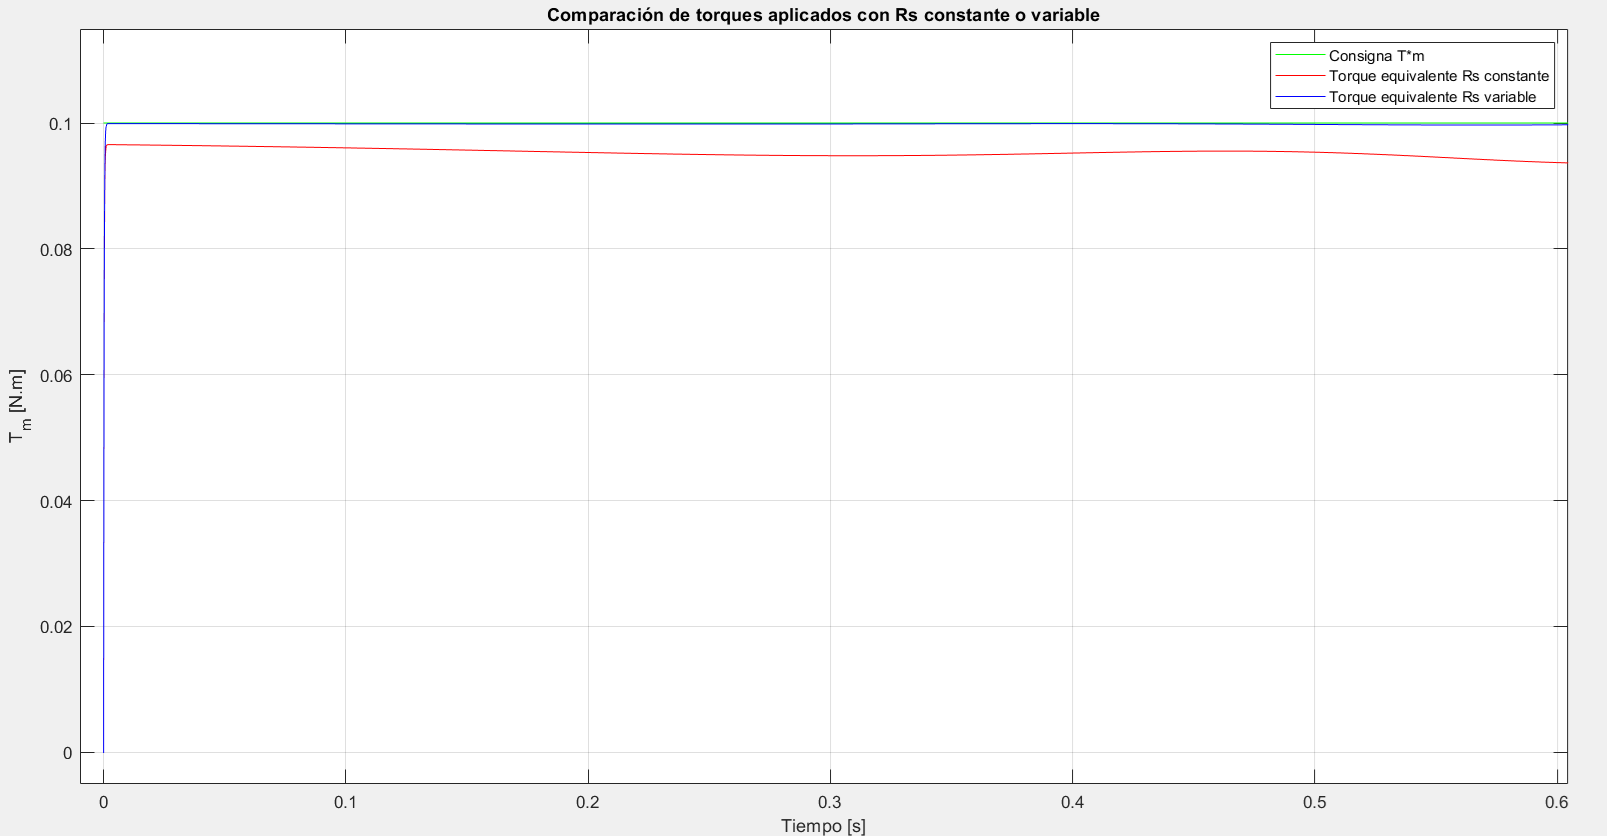
\includegraphics[width=0.85\textwidth]{Imagenes/ComparacionModuladorTorqueRs.png}
        \caption{Comparación entre el torque resultante aplicado sobre el eje mecánico considerando \(R_s\) constante (curva roja) o variable (curva azul).}
        \label{fig:ComparacionTorquesRs}
    \end{subfigure}
    
    \vspace{0.5cm} % Espacio entre subfiguras
    
    % Subfigura (b) - Bloque compacto
    \begin{subfigure}[t]{\textwidth}
        \centering
        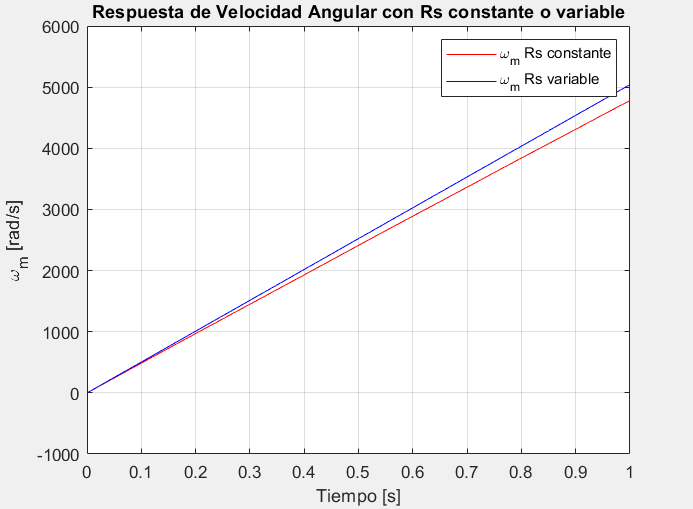
\includegraphics[width=0.65\textwidth]{Imagenes/ComparacionVelocidadModuladorRs.png}
        \caption{Comparación entre la velocidad angular obtenida del eje mecánico considerando \(R_s\) constante (curva roja) o variable (curva azul).}
        \label{fig:ComparacionVelocidadRs}
    \end{subfigure}
    
    \caption{Respuesta de Torque electromagnético \(T_m\) y velocidad angular \(\omega_m\) del eje mecánico de la máquina eléctrica considerando $R_s$ variable y constante.}
    \label{fig:ComparacionModuladorTorqueRs}
\end{figure}

\textbf{Diagrama de Bloques de la Realimentación para el Desacople de las Realimentaciones Físicas}

La Figura~\ref{fig:modulador_torque} muestra el diagrama de bloques de los desacoples de las realimentaciones físicas, en el cual se tiene en cuenta la variación de la temperatura del sistema (Ts(t)), por lo que la resistencia de los devanados del estator variaría con la temperatura, de este modo, replicando mejor el comportamiento real del sistema físico.

\begin{figure}[H]
    \centering
    % Subfigura (a) - Diagrama de bloques desagregado
    \begin{subfigure}[t]{\textwidth}
        \centering
        \includegraphics[width=0.7\textwidth]{Imagenes/modulador_torque_desacople_realimentaciones.png}
        \caption{Diagrama de bloques de la realimentación para el desacople de las realimentaciones físicas.}
        \label{fig:modulador_torque}
    \end{subfigure}
    
    \vspace{0.5cm} % Espacio entre subfiguras
    
    % Subfigura (b) - Bloque compacto
    \begin{subfigure}[t]{\textwidth}
        \centering
        \includegraphics[width=0.2\textwidth]{Imagenes/modulador_torque_desacople_realimentaciones_compacto.png}
        \caption{Bloque compacto de la realimentación para el desacople de las realimentaciones físicas.}
        \label{fig:modulador_torque_desacople_realimentaciones_compacto}
    \end{subfigure}
    
    \caption{Comparación entre el diagrama desagregado y el bloque compacto del desacople de las realimentaciones físicas.}
    \label{fig:modulador_torque_desacople_realimentaciones}
\end{figure}


\textbf{Lazos de Control de Corrientes \(\boldsymbol{i^r_{q d 0 s}(t)}\) con Control Proporcional}

Para que el modulador de torque equivalente pueda ejecutar correctamente las consignas de torque, es necesario asegurar control directo y preciso sobre las corrientes del estator en coordenadas rotóricas \( qd0 \). Hasta el momento, se logró un desacoplamiento interno que linealiza la relación entre las tensiones virtuales \((v_{qs}^{r*}(t), v_{ds}^{r*}(t), v_{0s}^{r*}(t))\) y las derivadas de las corrientes \((i_{qs}^r(t), i_{ds}^r(t), i_{0s}(t))\). Esto permite considerar cada eje \((q,d,0)\) como un subsistema dinámico sencillo (similar a un integrador).

A partir de esta situación, se implementan lazos de control proporcionales de corriente. La idea es que las tensiones de referencia \((v_{qs}^{r*}(t), v_{ds}^{r*}(t), v_{0s}^{r*}(t))\) se obtengan a partir del error entre las corrientes deseadas \((i_{qs}^{r*}(t), i_{ds}^{r*}(t), i_{0s}^{r*}(t))\) y las corrientes medidas \((i_{qs}^r(t), i_{ds}^r(t), i_{0s}(t))\), multiplicando dicho error por una ganancia proporcional adecuada. Así, para cada eje se tiene:

\[
L_q \frac{d i_{qs}^r(t)}{dt} \approx v_{qs}^{r*}(t) = (i_{qs}^{r*}(t) - i_{qs}^r(t)) R'_q,
\]
\[
L_d \frac{d i_{ds}^r(t)}{dt} \approx v_{ds}^{r*}(t) = (i_{ds}^{r*}(t) - i_{ds}^r(t)) R'_d,
\]
\[
L_{ls} \frac{d i_{0s}(t)}{dt} \approx v_{0s}^{r*}(t) = (i_{0s}^{r*}(t) - i_{0s}(t)) R'_0.
\]

Aquí, \(R'_q, R'_d, R'_0\) son constantes de proporcionalidad que, físicamente, pueden interpretarse como resistencias virtuales. Su elección determinará la ubicación de los polos del lazo de corriente.

\textbf{Aplicación de la Transformada de Laplace y Funciones de Transferencia}

Para analizar el comportamiento dinámico de estos lazos, aplicamos la transformada de Laplace a las ecuaciones anteriores. Por ejemplo, para el eje \(q\):

\[
L_q s I_{qs}(s) \approx (I_{qs}^{r*}(s) - I_{qs}(s)) R'_q.
\]

Reorganizando términos:

\[
L_q s I_{qs}(s) + R'_q I_{qs}(s) = R'_q I_{qs}^{r*}(s),
\]

\[
(L_q s + R'_q) I_{qs}(s) = R'_q I_{qs}^{r*}(s).
\]

La función de transferencia desde la corriente de referencia \(I_{qs}^{r*}(s)\) hasta la corriente real \(I_{qs}(s)\) es:

\[
G_{iqs}(s) = \frac{I_{qs}(s)}{I_{qs}^{r*}(s)} = \frac{R'_q}{L_q s + R'_q}.
\]

Dividiendo numerador y denominador por \(R'_q\):

\[
G_{iqs}(s) = \frac{1}{\frac{L_q}{R'_q} s + 1}.
\]

Análogamente, para los ejes \(d\) y \(0\):

\[
G_{ids}(s) = \frac{1}{\frac{L_d}{R'_d} s + 1}, \quad G_{i0s}(s) = \frac{1}{\frac{L_{ls}}{R'_0} s + 1}.
\]

Estas funciones de transferencia son típicas de sistemas de primer orden con ganancia estática unitaria y un polo real negativo. Cada lazo de corriente se comporta como un filtro pasa-bajos de primer orden, cuyo polo está determinado por la relación \(\frac{R'_q}{L_q}\), \(\frac{R'_d}{L_d}\), \(\frac{R'_0}{L_{ls}}\).

\textbf{Elección de Polos y Ganancias}

El objetivo es ubicar polos en \(p_i = -5000\,\text{rad/s}\) para todos los ejes, lo que implica:

\[
\frac{R'_q}{L_q} = 5000 \implies R'_q = 5000 L_q = 29 \Omega,
\]
\[
\frac{R'_d}{L_d} = 5000 \implies R'_d = 5000 L_d = 33 \Omega,
\]
\[
\frac{R'_0}{L_{ls}} = 5000 \implies R'_0 = 5000 L_{ls} = 4 \Omega.
\]

De esta forma, el ancho de banda del lazo de corriente se extiende hasta aproximadamente 796 Hz, asegurando una respuesta muy rápida frente a perturbaciones o cambios en las referencias.

\textbf{Interpretación y Comparación con el Ítem 5.1.2.c.VI}

En el ítem 5.1.2.c.VI se realizaba una linealización mínima mediante retroalimentación no lineal, imponiendo \( i_{ds}^r(t)=0 \) sin ubicar explícitamente polos para el lazo interno de corriente. Esto limitaba la capacidad de ajustar la rapidez de la respuesta interna.

Ahora, con el control proporcional de las corrientes, se introduce una forma explícita de control interno que permite:

\begin{itemize}
    \item Ajustar la velocidad de respuesta de las corrientes, haciéndola más rápida o lenta según convenga.
    \item Aumentar la robustez ante variaciones paramétricas (por ejemplo, debido a \(R_s(T_s^\circ)\)).
    \item Permitir \( i_{ds}^{r*}(t) \neq 0 \), abriendo la posibilidad de realizar debilitamiento o reforzamiento de campo, algo que no era posible bajo la condición \(i_{ds}^r(t)=0\).
\end{itemize}


\begin{figure}[H]
    \centering
    % Subfigura (a) - Diagrama de bloques desagregado
    \begin{subfigure}[t]{\textwidth}
        \centering
        \includegraphics[width=0.7\textwidth]{Imagenes/modulador_corriente.png}
        \caption{Diagrama de bloques del modulador de corriente.}
        \label{fig:modulador_corrientes}
    \end{subfigure}
    
    \vspace{0.5cm} % Espacio entre subfiguras
    
    % Subfigura (b) - Bloque compacto
    \begin{subfigure}[t]{\textwidth}
        \centering
        \includegraphics[width=0.2\textwidth]{Imagenes/modulador_corriente_compacto.png}
        \caption{Bloque compacto del modulador de corriente.}
        \label{fig:modulador_corriente_desacople_realimentaciones_compacto}
    \end{subfigure}
    
    \caption{Comparación entre el diagrama desagregado y el bloque compacto del modulador de corriente.}
    \label{fig:modulador_corriente}
\end{figure}


\newpage
\textbf{Incorporación de la Consigna de Torque y Compensación del Subsistema Mecánico}

Una vez determinados los lazos internos de corriente y el desacoplamiento electromagnético, se completa el modulador de torque equivalente incorporando la consigna de torque mecánico como nueva variable manipulada. Adicionalmente, se compensan las perturbaciones mecánicas internas: la fricción viscosa equivalente y el torque debido a la gravedad sobre la carga. Esta estrategia garantiza que el torque electromagnético que “ve” el lazo externo de control de movimiento no se vea afectado por dichas perturbaciones, facilitando su diseño y sintonía.

\textbf{Consigna de Torque con Compensación de Fricción Viscosa y Gravedad (Precomputed Torque)}

Partimos de una consigna de torque “pura” \(T_m^{*'}(t)\), correspondiente al torque mecánico deseado sin considerar pérdidas ni perturbaciones. Para incluir la fricción viscosa \( b_{eq} \,\omega_m(t) \) y el efecto de la gravedad sobre la carga, modificamos la consigna total de torque:

\begin{equation}
T_m^{*}(t) = T_m^{*'}(t) + b_{eq}\,\omega_m(t) + \frac{k_t}{r}\sin\left(\frac{\theta_m(t)}{r}\right).
\end{equation}

Con esta expresión, el modulador de torque genera internamente el torque adicional necesario para compensar la fricción viscosa y el torque gravitacional. De esta forma, el torque electromagnético resultante desde el punto de vista del lazo externo se aproxima a \(T_m^{*'}(t)\), liberando al controlador de movimiento de la tarea de contrarrestar estas perturbaciones mecánicas internas.

\textbf{Relación entre el Torque y las Corrientes}

El torque electromagnético en coordenadas \( qd \) se expresa como:

\begin{equation}
T_m(t) = \frac{3}{2} P_p [ \lambda_m' + (L_d - L_q)i_{ds}^r(t) ]\, i_{qs}^r(t),
\end{equation}

donde \(P_p\) es el número de pares de polos, \(\lambda_m'\) el flujo magnético del imán permanente, y \(L_d, L_q\) las inductancias en ejes d y q respectivamente.

Conocido \(T_m^{*}(t)\), podemos despejar la referencia de corriente en el eje q:

\begin{equation}
i_{qs}^{r*}(t) = \frac{T_m^{*'}(t) + b_{eq}\,\omega_m(t) + \frac{k_l \cdot g}{r}\sin\left(\frac{\theta_m(t)}{r}\right)}{\frac{3}{2}P_p[\lambda_m' + (L_d - L_q)i_{ds}^r(t)]}.
\label{eq:Consigna_Corriente_Modulador_Torque}
\end{equation}

\textbf{Casos Especiales y Flexibilidad}

- Si \( i_{ds}^r(t)=0 \), el torque depende sólo del flujo de imán permanente y la corriente q. Esta configuración simplifica la implementación y es suficiente en muchos casos.  
- Si \( i_{ds}^r(t)\neq 0 \), se puede modificar el campo magnético interno (field weakening/forcing), ampliando el rango de operación en torque y velocidad, a costa de mayor complejidad.

\begin{figure}[H]
    \centering
    % Subfigura (a) - Diagrama de bloques desagregado
    \begin{subfigure}[t]{\textwidth}
        \centering
        \includegraphics[width=0.7\textwidth]{Imagenes/modulador_torque.png}
        \caption{Diagrama de bloques del modulador de torque con compensaciones internas.}
        \label{fig:modulador_torque_1}
    \end{subfigure}
    
    \vspace{0.5cm} % Espacio entre subfiguras
    
    % Subfigura (b) - Bloque compacto
    \begin{subfigure}[t]{\textwidth}
        \centering
        \includegraphics[width=0.35\textwidth]{Imagenes/modulador_torque_compacto.png}
        \caption{Bloque compacto del modulador de torque.}
        \label{fig:modulador_torque_compacto}
    \end{subfigure}
    
    \caption{Comparación entre el diagrama detallado y su versión compacta del modulador de torque, incluyendo la incorporación de la consigna de torque, fricción viscosa y torque gravitacional.}
    \label{fig:subsistema_modulador_torque}
\end{figure}
\noindent\textbf{Simulación con Modulador de Torque}

A continuación se mostrarán los resultados obtenidos en la simulación en el dominio del tiempo del sistema global NL completo utilizando el modulador de Torque diseñado con el modulador de corriente en cascada y los desacoples de realimentaciones naturales correspondientes. 

En la Figura~\ref{fig:curvas_torques_modulador} se observan las señales en función del tiempo de: consigna de torque \(T^{*'}_m(t)\), Torque electromagnético \(T_m\), Torque equivalente aplicado sobre el eje mecánico de la máquina eléctrica, Torque de Perturbación \(T_l\), el cual involucra tanto la perturbación por posición angular de la articulación del brazo robótico cómo la perturbación por contacto \(T_{ld}(t)\), y el Torque por fricción viscosa. En la Figura~\ref{fig:acercamiento_torques_modulador} se puede ver cómo el torque total aplicado sobre el eje mecánico de la máquina eléctrica sigue al escalón de la consigna de torque \(T^{*'}_m(t)\). Para ello, el torque electromagnético necesario debe compensar los efectos del torque de perturbación \(T_l\) y el Torque por fricción viscosa \(b_{eq} \cdot \omega_m\). Para la simulación, se consideró una condición inicial para la posición angular no nula, \(\theta_m(0) \neq 0\) para provocar una perturbación por aceleración de la gravedad sobre el brazo robótico. Para la consigna de torque se consideró un valor consistente con los puntos de equilibrios obtenidos en la simulación DT de la sección~\ref{sec:respuesta_estado_interno_simulaciónDT}. Si este valor es muy grande, la simulación no se realiza correctamente, por lo cual se debe escoger un valor razonable.



\begin{figure}[H]
    \centering
    \begin{subfigure}[t]{\textwidth}
        \centering
        \includegraphics[width=0.7\textwidth]{Imagenes/Torques_simulacion_modulador_torque.png}
        \caption{Curvas de Consigna de Torque, Torque electromagnético, torque por fricción viscosa, torque de perturbación y torque total aplicado sobre el eje mecánico en función del tiempo.}
        \label{fig:curvas_torques_modulador}
    \end{subfigure}
    
    \vspace{0.5cm} % Espacio entre subfiguras
    
    \begin{subfigure}[t]{\textwidth}
        \centering
        \includegraphics[width=0.6\textwidth]{Imagenes/Acercamiento_torques_modulador.png}
        \caption{Acercamiento en el instante inicial \(t = 0\, s\) para observar escalón de consigna de torque \(T^{*'}_m(t) = 0{.}1\, Nm\) y la respuesta del Torque total aplicado sobre el eje mecánico del motor.}
        \label{fig:acercamiento_torques_modulador}
    \end{subfigure}
    \caption{Comparación de los distintos torques aplicados sobre la máquina eléctrica en el comportamiento dinámico de la simulación en el dominio del tiempo con Modulador de Torque.}
    \label{fig:simulacionDT_modulador_torques}
\end{figure}
\newpage
En la Figura~\ref{fig:curvas_posicion_velocidad_modulador_torque} se observan las curvas de posición y velocidad angular del eje mecánico, las cuales son consistentes con una consigna de torque constante. Un torque constante genera una aceleración angular de valor constante, y ésto a su vez, genera que la curva de velocidad angular tenga la forma de una recta lineal y la de la posición angular, una curva parabólica.

\begin{figure}[H]
    \centering
    \includegraphics[width=0.6\textwidth]{Imagenes/Curvas_posicion_velocidad_modular_torque.png}
    \caption{Curvas de posición y velocidad angular del eje mecánico de la máquina eléctrica, con modulador de torque equivalente y consigna de torque.}
    \label{fig:curvas_posicion_velocidad_modulador_torque}
\end{figure}

En la Figura~\ref{fig:simulacionDT_modulador_corrientes} se observa el comportamiento dinámico de las corrientes reales \(abc\), se puede comparar con la Figura~\ref{fig:curvas_torques_modulador} para ver como el torque electromagnético \(T_m(t)\) representa la envolvente de las curvas de corrientes. Las mismas seguirán creciendo sin límite ya que al tener una aceleración angular constante, el torque por fricción viscosa aumenta linealmente y el torque electromagnético debe compensar esta fricción para lograr la consigna de torque establecida. Esto en la práctica no debe ser así, ya que se superarán los valores de especificaciones de operación establecidos en el cuadro~\ref{tabla:especificaciones_operacion_electricas}.

\begin{figure}[H]
    \centering
    \begin{subfigure}[t]{0.48\textwidth}
        \centering
        \includegraphics[width=\textwidth]{Imagenes/Curvas_corrientes_modulador_torque.png}
        \caption{Corrientes en coordenadas reales \(abc\) con modulador de torque equivalente.}
        \label{fig:curvas_corrientesABC_modulador_torque}
    \end{subfigure}
    \hfill  % Esto agrega un espacio horizontal flexible entre las subfiguras
    \begin{subfigure}[t]{0.48\textwidth}
        \centering
        \includegraphics[width=\textwidth]{Imagenes/Acercamiento_corrientes_modulador_torque.png}
        \caption{Acercamiento de corrientes en coordenadas reales \(abc\) en el instante \(t = 0{.}4\, s\).}
        \label{fig:acercamiento_corrientes_torques_modulador}
    \end{subfigure}
    \caption{Respuesta de corrientes reales de la simulación DT con modulador de torque equivalente y consigna de torque.}
    \label{fig:simulacionDT_modulador_corrientes}
\end{figure}

De la ecuación~\ref{eq:Consigna_Corriente_Modulador_Torque}, vemos que considerar la estrategia \(i_{ds}^*(t) = 0\), genera el desacople entre los ejes virtuales \(q\) y \(d\) anulando los efectos de reforzamiento y debilitamiento de campo. Por ello, el torque electromagnético depende únicamente del flujo magnético generado por los imanes permanentes de la máquina.

Por otro lado, introducir corrientes \(i_{ds}^*(t) \neq 0\) genera los siguientes efectos:

\begin{itemize}
   \item Con \(i_{ds}^*(t) > 0\) se produce reforzamiento de campo: se visualiza un leve incremento en el torque electromagnético erogado por el motor.
   \item Con \(i_{ds}^*(t) < 0\) se produce debilitamiento de campo: se visualiza un leve decremento en el torque electromagnético erogado por el motor.
\end{itemize}

\subsection{Controlador externo de movimientos: posición/velocidad}

Con el fin de mejorar la dinámica del sistema y corregir los errores de estado estacionario producidos por cargas 
perturbadoras, se implementa un controlador que reciba consignas de velocidad y posición, y defina el torque necesario para 
tal acción. Será diseñado utilizando el método de sintonía serie con acción integral para el PID, con $\xi = 0,75$ y $\omega_n = 800\,  {rad/s}$, 
con valores nominales de inercia \(J_l\) y amortiguamiento \(b_l\).

Se optó por utilizar como variable de entrada, solo la velocidad angular del motor. Esto se realizó para evitar incluir acciones 
derivativas en el controlador, lo que podría resultar en errores numéricos debido a su acción como filtro pasa alto. Es decir, es 
más conveniente para evitar inestabilidades, integrar la realimentación de velocidad que derivar la realimentación de posición. De esta 
forma, el modelo emplea dos bloques integrales que actúan como filtros pasa bajos y eliminan el ruido proveniente del error 
de posición y velocidad, ya que por naturaleza son de alta frecuencia.

La salida del controlador será la consigna de torque que ingresará al modular de torque de la sección anterior, por lo tanto, 
modelando el sistema en el dominio de Laplace se tiene:

\begin{equation}
T_m^{*'}(s) = e_\omega(s).b_a + e_\theta(s).K_{sa} + K_{sia}\frac{e_\theta(s)}{s}
\label{eq:torque_controlador}
\end{equation}

Donde las variables $e_\theta(s)$ y $e_\omega(s)$ representan los errores entre las consignas de posición y velocidad angular, y el valor 
medido, respectivamente:

\begin{equation}
e_\theta(s) = \theta^*(s) - \theta(s)
\end{equation}

\begin{equation}
e_\omega(s) = e_\theta(s).s
\end{equation}

\begin{figure}[H]
    \centering
    % Subfigura (a) - Diagrama de bloques desagregado
    \begin{subfigure}[t]{0.6\textwidth}
        \centering
        \includegraphics[width=\textwidth]{Imagenes/DiagramaBloquesPIDdesagregado.png}
        \caption{Diagrama de bloques del controlador PID de movimiento con consigna de velocidad \(\omega^*_m\).}
        \label{fig:DiagramaBloquesPIDdesagregado}
    \end{subfigure}
    \hfill % Esto agrega un espacio horizontal flexible entre las subfiguras
    % Subfigura (b) - Bloque compacto
    \begin{subfigure}[t]{0.35\textwidth}
        \centering
        \includegraphics[width=\textwidth]{Imagenes/DiagramaBloquesPIDcompacto.png}
        \caption{Bloque compacto del controlador PID.}
        \label{fig:DiagramaBloquesPIDcompacto}
    \end{subfigure}
    
    \caption{Comparación entre el diagrama detallado y su versión compacta del controlador PID de movimiento.}
    \label{fig:DiagramaBloquesControladorPID}
\end{figure}

Por otro lado, la relación entre el torque y la variación de velocidad del motor en el modelo del subsistema mecánico, 
teniendo en cuenta el desacople de $-b_{eq}.\omega_m(t)$ de la sección anterior, se ve que:

\begin{equation}
J_{eq}.\dot{\omega}_m(t) = T_m^*(t) - \frac{T_l(t)}{r}
\end{equation}

Aplicando la transformada de Laplace y reemplazando en la ecuación del controlador, se tiene:
\begin{equation}
J_{eq} \cdot s^2 \cdot \theta_m(s) = T_m^*(s) - \frac{T_l(s)}{r}
\label{eq:laplace_mecanica}
\end{equation}

Sustituyendo la expresión del torque del controlador (Ec.~\ref{eq:torque_controlador}) y expandiendo los términos de error:
\begin{equation}
J_{eq} \cdot s^2 \cdot \theta_m(s) = E_\theta(s) \cdot s \cdot b_a + E_\theta(s) \cdot K_{sa} + \frac{E_\theta(s)}{s} \cdot K_{sia} - \frac{T_l(s)}{r}
\label{eq:sustitucion_torque}
\end{equation}

Reemplazando la expresión del error de posición $E_\theta(s) = [\theta_m^*(s) - \theta_m(s)]$:
\begin{equation}
J_{eq} \cdot s^2 \cdot \theta_m(s) = \left[s \cdot b_a + K_{sa} + \frac{K_{sia}}{s}\right] \cdot [\theta_m^*(s) - \theta_m(s)] - \frac{T_l(s)}{r}
\label{eq:reemplazo_error}
\end{equation}

Agrupando términos con $\theta_m(s)$ a la izquierda y términos con $\theta_m^*(s)$ y $T_l(s)$ a la derecha:
\begin{equation}
[J_{eq} \cdot s^3 + s^2 \cdot b_a + s \cdot K_{sa} + K_{sia}] \cdot \theta_m(s) = [s^2 \cdot b_a + s \cdot K_{sa} + K_{sia}] \cdot \theta_m^*(s) - \frac{T_l(s)}{r} \cdot s
\label{eq:agrupacion_terminos}
\end{equation}

Despejando $\theta_m(s)$:
\begin{equation}
\theta_m(s) = \frac{s^2 \cdot b_a + s \cdot K_{sa} + K_{sia}}{J_{eq} \cdot s^3 + s^2 \cdot b_a + s \cdot K_{sa} + K_{sia}} \cdot \theta_m^*(s) - \frac{s}{J_{eq} \cdot s^3 + s^2 \cdot b_a + s \cdot K_{sa} + K_{sia}} \cdot \frac{T_l(s)}{r}
\label{eq:theta_despejada}
\end{equation}

De esta ecuación podemos identificar las funciones de transferencia del sistema. Para la entrada de consigna de posición $\theta_m^*(s)$:
\begin{equation}
G_{\theta^*_m}(s) = \frac{\theta_m(s)}{\theta_m^*(s)} = \frac{s^2 \cdot b_a + s \cdot K_{sa} + K_{sia}}{J_{eq} \cdot s^3 + s^2 \cdot b_a + s \cdot K_{sa} + K_{sia}}
\label{eq:FT_consigna}
\end{equation}

Y para la perturbación de torque $T_l(s)$:
\begin{equation}
G_{T_l}(s) = \frac{\theta_m(s)}{\frac{T_l(s)}{r}} = -\frac{s}{J_{eq} \cdot s^3 + s^2 \cdot b_a + s \cdot K_{sa} + K_{sia}}
\label{eq:FT_perturbacion}
\end{equation}

La ecuación (\ref{eq:FT_consigna}) representa cómo la posición del motor responde a cambios en la consigna de posición, mientras que la ecuación (\ref{eq:FT_perturbacion}) describe cómo la posición se ve afectada por perturbaciones en el torque de carga. Estas funciones de transferencia serán fundamentales para analizar el comportamiento del sistema en diferentes condiciones de operación.

Si analizamos las funciones de transferencia en régimen estacionario para una entrada escalón unitario:

\begin{itemize}
\item Si $K_{sia} \neq 0 \rightarrow G_{\theta^*}(s) = 1$ y $G_{T_l}(s) = 0$ (rechazo total a perturbaciones)
\item Si $K_{sia} = 0 \rightarrow G_{\theta^*}(s) = 1$ y $G_{T_l}(s) = -1/K_{sa}$ (sin rechazo a perturbaciones)
\end{itemize}

Con esto se observa cómo la acción integral es capaz de corregir el error en estado estacionario producto de las 
perturbaciones en el torque de carga.

Ahora se deben encontrar los valores óptimos de las ganancias del controlador, utilizando el método de sintonía serie con 
$n=2.5$. Se tiene:

\begin{equation}
\omega_{vel} = \frac{b_a}{J_{eq}} \qquad \omega_{pos} = \frac{K_{sa}}{b_a} \qquad \omega_{int} = \frac{K_{sia}}{K_{sa}}
\label{eq:frecuencias_caracteristicas}
\end{equation}

Sabiendo que:
\begin{equation}
\omega_{vel} = n \cdot \omega_{pos} \qquad \omega_{int} = \frac{1}{n} \cdot \omega_{pos}
\label{eq:relacion_frecuencias}
\end{equation}

Tenemos finalmente, con $\omega$ como frecuencia que se impone a los polos y representa el ancho de banda del controlador, 
$\omega = 800 \frac{rad}{s}$; $n = 2.5$; y considerando la inercia equivalente variable según:

\begin{equation}
J_{eq} = J_m + \frac{J_l}{r^2}
\label{eq:inercia_equivalente}
\end{equation}

Donde $J_m = 14\times10^{-6}$ kg.m², $r = 120$ y $J_l$ varía entre 0.0833 y 0.4583 kg.m².

Para el caso nominal ($J_{eq} = 1{.}9785\times10^{-5}$ kg.m² para \(J_l = 0.0833 \text{kg.m²}\) dado \(m_l = 0\)), las ganancias del controlador resultan:

\begin{equation}
b_a = J_{eq} \cdot n \cdot \omega_{pos} = 0.039 \frac{N\cdot m}{rad/s}
\label{eq:ganancia_ba}
\end{equation}

\begin{equation}
K_{sa} = J_{eq} \cdot n \cdot \omega_{pos}^2 = 31.656 \frac{N\cdot m}{rad}
\label{eq:ganancia_ksa}
\end{equation}

\begin{equation}
K_{sia} = J_{eq} \cdot \omega_{pos}^3 = 10129.78 \frac{N\cdot m}{rad\cdot s}
\label{eq:ganancia_ksia}
\end{equation}

Con estos datos podemos obtener el polinomio característico del controlador:
\begin{equation}
p(s) = J_{eq} \cdot s^3 + b_a \cdot s^2 + K_{sa} \cdot s + K_{sia} = J_{eq} \cdot (s + \omega_{pos}) \cdot (s^2 + (n-1) \cdot \omega_{pos} \cdot s + \omega_{pos}^2)
\label{eq:polinomio_caracteristico}
\end{equation}

Comparando esto con la forma normalizada del polinomio de 3er grado factorizado en 2 términos:
\begin{equation}
(s + \omega_n) \cdot (s^2 + 2 \cdot s \cdot \xi \cdot \omega_n + \omega_n^2)
\label{eq:forma_normalizada}
\end{equation}

Sabiendo que la distancia radial al origen es la misma para los 3 polos, lo que representa un filtro de Butterworth de tercer 
orden; vemos que para los distintos valores de $J_{eq}$:

Para valores nominales de $J_{eq}$:
\begin{equation}
\xi = \frac{n-1}{2} = 0.75 \quad s_1 = -800\frac{rad}{s} \quad s_{2,3} = -600 \pm 529.15\,i \frac{rad}{s}
\label{eq:polos_nominal}
\end{equation}

Para valores máximos de $J_{eq}$:
\begin{equation}
s_1 = -464.44\frac{rad}{s} \quad s_{2,3} = -464.44 \pm 673.18\,i \frac{rad}{s}
\label{eq:polos_max}
\end{equation}

\newpage

En la Figura~\ref{fig:migracion_polos_controlador} se observan los polos del sistema con el controlador, con el regulador de corriente, y los polos de la planta original:

\begin{figure}[H]
    \centering
    \includegraphics[width=0.95\textwidth]{Imagenes/MigracionPolosControlador.png}
    \caption{Polos del controlador variando \(J_{eq}\) y \(b_{eq}\), junto con polos a lazo abierto de la planta y polo del lazo de corriente.}
    \label{fig:migracion_polos_controlador}
\end{figure}


\textbf{Entrada de referencia o setpoint de posición}

Finalmente, para concluir esta sección, se incorpora la posibilidad de implementar el control de posición mediante una entrada de referencia. Esto permite emplear algoritmos en el control de la articulación. Dicho planteamiento se representa mediante el siguiente modelo:

\[
q_1^*(t) = \frac{1}{r} \cdot \theta_m^*(t) \tag{Ec. 77}
\]

Además, se realizarán las modificaciones necesarias para que, a partir de esta consigna de posición, sea posible obtener una consigna de velocidad mediante la derivada de la misma. Esta derivación puede realizarse sin amplificar el error causado por el ruido electromagnético, ya que en este caso no se trata de una variable medida, sino de una consigna. Cabe destacar que el ruido, en sí mismo, proviene del sensado de las variables y del transporte de la señal a lo largo de los cables, entre otros factores. Por lo tanto, no hay inconvenientes al llevar a cabo esta operación.

\begin{figure}[H]
    \centering
    % Subfigura (a) - Diagrama de bloques desagregado
    \begin{subfigure}[t]{0.5\textwidth}
        \centering
        \includegraphics[width=\textwidth]{Imagenes/setpoint.png}
        \caption{Diagrama de bloques del setpoint de posición \(\theta_m^*\).}
        \label{fig:setpoint}
    \end{subfigure}
    \hfill % Esto agrega un espacio horizontal flexible entre las subfiguras
    % Subfigura (b) - Bloque compacto
    \begin{subfigure}[t]{0.2\textwidth}
        \centering
        \includegraphics[width=\textwidth]{Imagenes/setpoint_compacto.png}
        \caption{Bloque compacto del setpoint de posición \(\theta_m^*\).}
        \label{fig:setpoint_compacto}
    \end{subfigure}
\end{figure}


\subsection{Observador de Estado de Orden Reducido}

El observador de estado de orden reducido se diseñó con el propósito de estimar la velocidad angular del motor a partir de la posición medida, ya que no se cuenta con un sensor de velocidad directa. Este estimador permite realimentar la velocidad angular para el control externo, optimizando el diseño del sistema al evitar la necesidad de sensores adicionales. Dado que el sistema no es observable desde la velocidad angular, es necesario estimarla utilizando la medición de posición angular.

\textbf{Modelo del Subsistema Mecánico}

El modelo del subsistema mecánico, ya desacoplado del término \(-b_{eq} \cdot \omega_m(t)\), se considera en el espacio de estados:

\[
\begin{aligned}
    \dot{\theta}_m(t) &= \omega_m(t), \\
    \dot{\omega}_m(t) &= \frac{1}{J_{eq}} \left(T_m'(t) - \frac{1}{r} T_l(t) \right),
\end{aligned}
\]

En forma matricial, el sistema se representa como:

\[
\dot{x}(t) = 
\begin{bmatrix}
0 & 1 \\ 
0 & 0
\end{bmatrix} 
x(t) + 
\begin{bmatrix}
0 \\ 
\frac{1}{J_{eq}}
\end{bmatrix} 
u(t),
\]
\[
y(t) = 
\begin{bmatrix}
1 & 0
\end{bmatrix} 
x(t),
\]

donde:
\[
x(t) = 
\begin{bmatrix}
\theta_m(t) \\ 
\omega_m(t)
\end{bmatrix}, \quad
u(t) = T_m'(t), \quad
y(t) = \theta_m(t), \quad
x(0) = 
\begin{bmatrix}
\theta_m(0) \\ 
\omega_m(0)
\end{bmatrix}.
\]


\textbf{Estados Iniciales}

Los estados iniciales del sistema son cruciales para garantizar la correcta convergencia del observador. El sistema físico tiene valores iniciales \(x(0) = \begin{bmatrix} \theta_m(0) \\ \omega_m(0) \end{bmatrix}\), mientras que el observador comienza con estados nulos (\(\tilde{x}(0) = \begin{bmatrix} 0 \\ 0 \end{bmatrix}\)), generando un error inicial:
\[
e(0) = x(0) - \tilde{x}(0).
\]
Este error inicial es corregido por la dinámica del observador, garantizando que \(e(t) \to 0\) de manera exponencial debido a los polos seleccionados.

\textbf{Diseño del Observador}

El observador de estado reducido se basa en la estructura de Luenberger, donde la dinámica del observador se corrige mediante un término proporcional al error entre la salida medida y la salida estimada:


\[
\dot{\tilde{x}}(t) = 
\begin{bmatrix}
0 & 1 \\ 
0 & 0
\end{bmatrix} 
\tilde{x}(t) + 
\begin{bmatrix}
0 \\ 
\frac{1}{J_{eq}}
\end{bmatrix} 
u(t) + 
\begin{bmatrix}
K_{e\theta} \\ 
K_{e\omega}
\end{bmatrix} 
\left( y(t) - 
\begin{bmatrix}
1 & 0
\end{bmatrix} 
\tilde{x}(t) \right),
\]

\[
\tilde{y}(t) = 
\begin{bmatrix}
1 & 0
\end{bmatrix} 
\tilde{x}(t).
\]


El error entre los estados reales y estimados se define como:
\[
e(t) = x(t) - \tilde{x}(t), \quad e(0) = x(0),
\]
cuya dinámica está dada por:
\[
\dot{e}(t) = \left( A - K_e C \right) e(t).
\]

\textbf{Cálculo de \( K_e \)}

La matriz \( A - K_e C \) tiene la forma:
\[
A - K_e C = \begin{bmatrix} 
-K_{e\theta} & 1 \\ 
-K_{e\omega} & 0 
\end{bmatrix}.
\]

El polinomio característico es:
\[
p(s) = \det\left(sI - (A - K_e C)\right) = s^2 + K_{e\theta}s + K_{e\omega}.
\]

Para \( p_{\text{obs}} = -3200 \, \text{rad/s} \), el polinomio característico deseado es:
\[
p_{\text{obs}}(s) = (s + 3200)^2 = s^2 + 6400s + 3200^2.
\]

Comparando coeficientes:
\[
K_{e\theta} = 6400 \, \text{rad/s}, \quad K_{e\omega} = 1.024 \times 10^7 \, \text{rad/s}^2.
\]

\textbf{Justificación de los Polos}

La elección de polos reales e iguales en \(-3200 \, \text{rad/s}\) asegura una rápida convergencia del observador sin generar oscilaciones. Estos polos están ubicados lo suficientemente alejados de los polos del controlador externo para no interferir con su dinámica. Esto garantiza un tiempo de establecimiento corto del observador y una correcta estimación de \(\tilde{\omega}_m(t)\).

\textbf{Diagrama de Bloques del Observador}

\begin{figure}[H]
    \centering
    % Subfigura (a) - Diagrama de bloques desagregado
    \begin{subfigure}[t]{0.7\textwidth}
        \centering
        \includegraphics[width=\textwidth]{Imagenes/observador.png}
        \caption{Diagrama de bloques del observador de estado reducido.}
        \label{fig:observador}
    \end{subfigure}
    \hfill % Esto agrega un espacio horizontal flexible entre las subfiguras
    % Subfigura (b) - Bloque compacto
    \begin{subfigure}[t]{0.2\textwidth}
        \centering
        \includegraphics[width=\textwidth]{Imagenes/observador_compacto.png}
        \caption{Bloque compacto del observador de estado reducido.}
        \label{fig:observador_compacto}
    \end{subfigure}
\end{figure}

\textbf{Análisis del Error}

La dinámica del error está gobernada por:
\[
\dot{e}(t) = (A - K_e C) e(t),
\]
donde \( A - K_e C \) es estable por construcción, con polos en \(-3200 \, \text{rad/s}\). Esto asegura que:
\[
\lim_{t \to \infty} e(t) = 0,
\]
es decir, el error del observador converge a cero en estado estacionario.

Con este diseño, el observador proporciona estimaciones precisas de la velocidad angular, permitiendo al controlador de movimiento operar eficientemente.



\subsection{Simulación en tiempo continuo con modelo completo NL}

Para realizar una simulación del sistema en tiempo continuo, realizamos una integración de todos los bloques presentados
anteriormente. El modelo de Simulink obtenido se observa Figura~\ref{fig:modelo_completo_simulacion}. Entre los bloques empleados podemos
distinguir aquellos que son parte de la planta: el subsistema electromagnético, el subsistema mecánico y el subsistema térmico.
También vemos los bloques que son parte del control: controlador de movimiento PID, modulador de torque y el observador
de estado reducido. La interfaz entre la planta y el control está dada por los elementos sensores, representados con ganancias
unitarias y por el elemento actuador, que en nuestro caso es el modulador de tensión, el cual toma las consignas de tensión y
las convierte en tensiones en los bornes de la máquina. En este caso, dicho modulador es representado por ganancias unitarias.

En principio se analizara los resultados obtenidos en el seguimiento de consignas de movimiento 
$q^*(t) \equiv \frac{1}{n}\theta_m(t)$ con perfil trapezoidal de posición. Se ensayara al sistema, con un perfil trapezoidal 
de posición con un tiempo de rampa $\Delta t_{ramp} = 5s$ y un posición final $q^*(\Delta t_{ramp}) = 2\pi$. Es decir se 
solicita una vuelta completa en sentido antihorario de la articulación del robot en $5s$ y luego una vuelta en sentido horario de 
igual manera.

\begin{figure}[H]
    \centering
    \includegraphics[width=1\textwidth]{Imagenes/Modelo_Completo_Simulacion.png}
    \caption{Diagrama de bloques del modelo completo con controlador de movimiento PID, modulador de torque y observador de estado reducido.}
    \label{fig:modelo_completo_simulacion}
\end{figure}
\newpage
\subsubsection{Seguimiento de consignas de movimiento.}

En la Figura~\ref{fig:ModeloCompletoConsignas} se observan las consignas de movimiento especificadas en la guía del Trabajo Integrador para la simulación del modelo completo en el dominio del tiempo. Las consignas de movimiento están referenciadas a la articulación del brazo robótico, por lo que las consignas de movimiento del eje de la máquina eléctrica están afectadas por el factor \(r \equiv 120\) de reducción del tren de transmisión. 

\begin{figure}[H]
    \centering
    \begin{subfigure}[b]{0.48\textwidth}
        \centering
        \includegraphics[width=\textwidth]{Imagenes/ConsignasMovimientoArticulacionRobotica.png}
        \caption{Consignas de movimiento para la articulación robótica especificadas en la consigna del Trabajo Integrador.}
        \label{fig:ConsignasMovimientoArticulaconRobotica}
    \end{subfigure}
    \hfill
    \begin{subfigure}[b]{0.48\textwidth}
        \centering
        \includegraphics[width=\textwidth]{Imagenes/ConsignasMovimientoMaquinaElectrica.png}
        \caption{Consignas de movimiento para el eje mecánico de la máquina eléctrica que están afectados por la relación de transmisión del tren de engranajes \(r \equiv 120\).}
        \label{fig:ConsignasMovimientoMaquinaElectrica}
    \end{subfigure}
    \caption{Consignas de movimiento para la simulación del modelo completo en el dominio del tiempo.}
    \label{fig:ModeloCompletoConsignas}
\end{figure}

En la Figura~\ref{fig:RespuestaPosicionVelocidadSimulacionCompleta} se observa que la consigna de posición se cumple satisfactoriamente, más allá de los transitorios en cada cambio brusco de la consigna de velocidad. A través de la Figura~\ref{fig:AcercamientoRespuestaSimulacionCompleta}, que es un acercamiento en el instante \(t = 5\,s\), se logra apreciar un pequeño error de \(0{.}005\) radianes entre la posición angular medida y la consigna de posición del eje mecánico de la máquina eléctrica. También se observa en la Figura los errores de estimación de posición y velocidad del Observador de Estado Reducido.

El sistema físico en la realidad sería incapaz de seguir esta consigna trapezoidal de posición ya que dicho perfil solicitado resulta en una curva de velocidad discontinua, lo que implica aceleraciones infinitas y por lo tanto torques, corrientes y tensiones muy elevadas que superan los límites especificados en el Cuadro~\ref{tabla:especificaciones_operacion_electricas}. Otra complicación que presenta este perfil de posición con puntos agudos y derivadas discontinuas es que aún cuando se pudieran aplicar los niveles de tensión necesarios a través del modulador de tensión trifásico para satisfacer la consigna, es que en un brazo robótico se busca reducir al máximo las aceleraciones por los esfuerzos dinámicos que estas provocan en las articulaciones. Teniendo en cuenta que el perfil de posición impuesto no es práctico por lo explicado anteriormente, sería útil implementar como restricción en el controlador que la consigna de velocidad no tenga discontinuidades.


\begin{figure}[H]
    \centering
    \begin{subfigure}[t]{\textwidth}
        \centering
        \includegraphics[width=0.8\textwidth]{Imagenes/PosicionVelocidadSimulacionModeloCompleto.png}
        \caption{Curvas de consignas de posición y velocidad (\(\theta^*_m\) y \(\omega^*_m\)), posición y velocidad  medidas (\(\theta_m\) y \(\omega_m\))  y posición y velocidad estimadas con el observador de estado reducido (\(\theta_{obs}\) y \(\omega_{obs}\)).}
        \label{fig:PosicionVelocidadSimulacionModeloCompleto}
    \end{subfigure}
    
    \vspace{0.5cm} % Espacio entre subfiguras
    
    \begin{subfigure}[t]{\textwidth}
        \centering
        \includegraphics[width=0.8\textwidth]{Imagenes/AcercamientoRespuestaSimulacionCompleta.png}
        \caption{Acercamiento en el instante \(t = 5\,s\) para observar los transitorios de posición y velocidad.}
        \label{fig:AcercamientoRespuestaSimulacionCompleta}
    \end{subfigure}
    \caption{Respuesta de posición y velocidad angular del eje mecánico de la máquina eléctrica en el seguimiento de las consignas.}
    \label{fig:RespuestaPosicionVelocidadSimulacionCompleta}
\end{figure}

\begin{figure}[H]
    \centering
    \includegraphics[width=0.45\textwidth]{Imagenes/ErroresObservadorSimulacionCompleta.png}
    \caption{Error de posición y velocidad por estimación de Observador de Estado de Orden Reducido.}
    \label{fig:ErroresObservadorSimulacionCompleta}
\end{figure}

En las Figuras~\ref{fig:TensionesSimulacionCompleta} y~\ref{fig:CorrientesSimulacionCompleta} se verifica lo detallado anteriormente, en la figura~\ref{fig:AcercamientoTensionesEstacionariasSimulacion} se observa el comportamiento senoidal de las tensiones aplicadas en los puntos de equilibrio de la simulación, y lo mismo en la figura~\ref{fig:AcercamientoCorrientesEstacionariasSimulacion} con las corrientes. En la figura~\ref{fig:AcercamientoCorrientesTransitoriosSimulacion} se observa que se presentan picos muy elevados en los transitorios que superan las especificaciones de operación eléctricas. Por otro lado, en la práctica el modulador de tensión llegaría a la saturación y no podría entregar tensiones tan elevadas en los transitorios como las que se ven en la figura~\ref{fig:AcercamientoTensionesTransitoriosSimulacion}.    

\begin{figure}[H]
    \centering
    \begin{subfigure}[t]{\textwidth}
        \centering
        \includegraphics[width=0.5\textwidth]{Imagenes/TensionesSimulacionCompleta.png}
        \caption{Curvas de tensiones en coordenadas virtuales \(qd0^r\) y absolutas \(abc\).}
        \label{fig:TensionesSimulacionCompleta}
    \end{subfigure}
    
    \vspace{0.5cm} % Espacio entre subfiguras
    
    \begin{subfigure}[t]{\textwidth}
        \centering
        \includegraphics[width=0.5\textwidth]{Imagenes/AcercamientoTensionesEstacionariasSimulacion.png}
        \caption{Acercamiento para observar las tensiones en los estados de equilibrio de la simulación.}
        \label{fig:AcercamientoTensionesEstacionariasSimulacion}
    \end{subfigure}

    \vspace{0.5cm} % Espacio entre subfiguras
    
    \begin{subfigure}[t]{\textwidth}
        \centering
        \includegraphics[width=0.5\textwidth]{Imagenes/AcercamientoTensionesTransitoriosSimulacion.png}
        \caption{Acercamiento en el instante \(t = 5\,s\) para observar las tensiones en los transitorios.}
        \label{fig:AcercamientoTensionesTransitoriosSimulacion}
    \end{subfigure}
    \caption{Curvas de Tensión en coordenadas virtuales y absolutas de la simulación del modelo completo en el dominio del tiempo.}
    \label{fig:TensionesSimulacionCompleta}
\end{figure}

\begin{figure}[H]
    \centering
    \begin{subfigure}[t]{\textwidth}
        \centering
        \includegraphics[width=0.5\textwidth]{Imagenes/CorrientesSimulacionCompleta.png}
        \caption{Curvas de corrientes en coordenadas virtuales \(qd0^r\) y absolutas \(abc\).}
        \label{fig:CorrientesSimulacionCompleta}
    \end{subfigure}
    
    \vspace{0.5cm} % Espacio entre subfiguras
    
    \begin{subfigure}[t]{\textwidth}
        \centering
        \includegraphics[width=0.5\textwidth]{Imagenes/AcercamientoCorrientesEstacionariasSimulacion.png}
        \caption{Acercamiento para observar las corrientes en los estados de equilibrio de la simulación.}
        \label{fig:AcercamientoCorrientesEstacionariasSimulacion}
    \end{subfigure}

    \vspace{0.5cm} % Espacio entre subfiguras
    
    \begin{subfigure}[t]{\textwidth}
        \centering
        \includegraphics[width=0.5\textwidth]{Imagenes/AcercamientoCorrientesTransitoriosSimulacion.png}
        \caption{Acercamiento en el instante \(t = 5\,s\) para observar los picos de corrientes en los transitorios.}
        \label{fig:AcercamientoCorrientesTransitoriosSimulacion}
    \end{subfigure}
    \caption{Curvas de Corrientes en coordenadas virtuales y absolutas de la simulación del modelo completo en el dominio del tiempo.}
    \label{fig:CorrientesSimulacionCompleta}
\end{figure}

\newpage
\subsubsection{Rechazo a Perturbaciones.}
\label{sec:rechazo_perturbaciones}

En este apartado, se evalúa el desempeño del sistema frente a perturbaciones de carga. Para ello se aplica una entrada
escalón en \( t = 0\,s\) con magnitud de \(T_{ld} = 5\,\text{N.m}\), y consigna de posición \(q^*(t) = 0\). Esto generó un error de estado
estacionario en la posición angular del motor. En la Figura~\ref{fig:RechazoPerturbacionesSimulacionCompleta} se observa el comportamiento del sistema frente a la consigna de posición con perturbación por contacto:

\begin{figure}[H]
    \centering
    \includegraphics[width=0.6\textwidth]{Imagenes/RechazoPerturbacionesSimulacionCompleta.png}
    \caption{Comportamiento del sistema frente a una consigna de posición \(q^*(t) = 0\) y perturbación por contacto \(T_{ld} = 5\,\text{N.m}\).}
    \label{fig:RechazoPerturbacionesSimulacionCompleta}
\end{figure}

El error es muy pequeño ya que la magnitud del torque de perturbación por contacto está afectado por la relación de la caja reductora.

\begin{figure}[H]
    \centering
    % Subfigura (a) - Diagrama de bloques desagregado
    \begin{subfigure}[t]{0.45\textwidth}
        \centering
        \includegraphics[width=\textwidth]{Imagenes/ErrorPosicionPerturbacion.png}
        \caption{Error de posición \(\theta^*(t)-\theta_m(t)\).}
        \label{fig:ErrorPosicionPerturbacion}
    \end{subfigure}
    \hfill % Esto agrega un espacio horizontal flexible entre las subfiguras
    % Subfigura (b) - Bloque compacto
    \begin{subfigure}[t]{0.45\textwidth}
        \centering
        \includegraphics[width=\textwidth]{Imagenes/AcercamientoErrorPosicionPerturbacion.png}
        \caption{Acercamiento en el intervalo [18\,s,20\,s].}
        \label{fig:AcercamientoErrorPosicionPerturbacion}
    \end{subfigure}
    \caption{Error de posición con Observador de Estado Reducido.}
    \label{fig:Error_posicion_observador_Reducido}
\end{figure}

Dicho error se debe a que el observador de estado planteado solo actúa de forma PD (proporcional derivativa), y no es capaz
de corregir dicho error de baja frecuencia. Esto implica que se debe mejorar el observador.

\section{Verificación de Desempeño y/o Mejoras}

\subsection{Especificaciones de Operación}
\label{sec:mejora_consignas_velocidades_trapezoidales}

Se realizó la verificación de las especificaciones de operación del sistema físico, incluyendo los valores límite de velocidad, torque, corriente y tensión de los componentes principales del motor, inversor y caja reductora. En la Tabla~\ref{tab:specifications}, se comparan los valores nominales con los resultados obtenidos en las simulaciones.

\begin{table}[H]
    \centering
    \caption{Comparación de valores simulados contra especificaciones de operación}
    \label{tab:specifications}
    \begin{tabular}{|c|c|c|c|c|}
        \hline
         & \multicolumn{2}{|c|}{\textbf{Especificación de Operación}} & \multicolumn{2}{|c|}{\textbf{Valores obtenidos en simulación}} \\ \hline
        \textbf{Especificación} & \textbf{Régimen Continuo} & \textbf{Máximo (Pico)} & \textbf{Régimen Continuo} & \textbf{Máximo (Pico)} \\ \hline
        Torque (Caja) & 17.0 N.m & 45.0 N.m & 2.85 N.m & 1492.8 N.m \\ \hline
        Velocidad Angular (Caja) & 6.28 rad/s & 6.28 rad/s & 1.25 rad/s & 1.88 rad/s \\ \hline
        Velocidad Angular (Motor) & 691.15 rad/s & 691.15 rad/s & 150 rad/s & 226.1 rad/s \\ \hline
        Corriente (Estator) & 0.4 A & 2.0 A & 0.34 A & 209 A \\ \hline
        Tensión de Fase (Estator) & 17.32 V & 27.71 V & 7.61 V & 62,000 V \\ \hline
    \end{tabular}
\end{table}

\textbf{Propuesta de mejora:} 
Para mitigar los valores que superan los límites, se propone implementar un perfil trapezoidal de velocidad. Este ajuste suaviza las aceleraciones, mejorando el comportamiento dinámico del sistema.
En la Figura~\ref{fig:perfil_trapezoidal_velocidad} se observan las nuevas consignas de posición y velocidad. A partir de la consigna inicial de velocidad \(\frac{dq_l}{dt}(t)^*\) se reemplazaron los saltos discretos de velocidad por rectas lineales en intervalos ajustados a gusto, modificando la forma de escalones de la consigna de velocidad por un perfil trapezoidal. Esta corrección en el perfil de velocidad elimina los valores elevados de aceleración y torque electromagnético, reduciendo los picos de corriente y tensiones máximas en los transitorios.



\begin{figure}[H]
    \centering
    % Subfigura (a) - Diagrama de bloques desagregado
    \begin{subfigure}[t]{0.55\textwidth}
        \centering
        \includegraphics[width=\textwidth]{Imagenes/perfil_trapezoidal_velocidad.png}
        \caption{Nuevas consignas de posición y velocidad angular de la articulación robótica con cambios de velocidad suavizados.}
        \label{fig:perfil_trapezoidal_velocidad}
    \end{subfigure}
    \hfill % Esto agrega un espacio horizontal flexible entre las subfiguras
    % Subfigura (b) - Bloque compacto
    \begin{subfigure}[t]{0.4\textwidth}
        \centering
        \includegraphics[width=\textwidth]{Imagenes/Acercamiento_perfil_trapezoidal_velocidad.png}
        \caption{Acercamiento en el instante \(t = 5\,s\).}
        \label{fig:Acercamiento_perfil_trapezoidal_velocidad}
    \end{subfigure}
\end{figure}

En la Figura~\ref{fig:Torque_electromagnetico_velocidad_trapezoidal} se observa el torque electromagnético \(T_m(t)\) obtenido con el nuevo perfil de velocidad, los picos máximos de torque de salida \(T_q(t) = r\cdot T_d(t)\) que antes llegaban a valores de 1492.8 N.m ahora valen 5.016 N.m.

En la Figura~\ref{fig:Corrientes_velocidad_trapezoidal} se observa una reducción muy importante de los picos de corriente en los bobinados del estator en los instantes de cambio de la velocidad en relación, a la simulación con el perfil de velocidad original sin suavizar.

Finalmente, en la Figura~\ref{fig:Tensiones_velocidad_trapezoidal} se observa que los valores máximos de tensión aplicada en los bobinados del estator de la máquina eléctrica se redujeron significativamente. El máximo valor de tensión en los transitorios es de 13.85 V, mucho menor que el valor obtenido en la Tabla~\ref{tab:specifications}

\begin{figure}[H]
    \centering
    \begin{subfigure}[t]{\textwidth}
        \centering
        \includegraphics[width=0.6\textwidth]{Imagenes/Torque_electromagnetico_velocidad_trapezoidal.png}
        \caption{Curva de Torque Electromagnético \(T_m(t)\) con el nuevo perfil de velocidad.}
        \label{fig:Torque_electromagnetico_velocidad_trapezoidal}
    \end{subfigure}
    
    \vspace{0.5cm} % Espacio entre subfiguras
    
    \begin{subfigure}[t]{\textwidth}
        \centering
        \includegraphics[width=0.6\textwidth]{Imagenes/Corrientes_velocidad_trapezoidal.png}
        \caption{Curva de corrientes virtuales y reales con el nuevo perfil de velocidad.}
        \label{fig:Corrientes_velocidad_trapezoidal}
    \end{subfigure}

    \vspace{0.5cm} % Espacio entre subfiguras
    
    \begin{subfigure}[t]{\textwidth}
        \centering
        \includegraphics[width=0.6\textwidth]{Imagenes/Tensiones_velocidad_trapezoidal.png}
        \caption{Curva de tensiones virtuales y reales con el nuevo perfil de velocidad.}
        \label{fig:Tensiones_velocidad_trapezoidal}
    \end{subfigure}
    \caption{Curvas de Torque Electromagnético, corrientes y tensiones obtenidas con el nuevo perfil de velocidad suavizado.}
    \label{fig:simulacion_perfil_trapezoidal_velocidad}
\end{figure}

\subsection{Observador de Estado}


En las simulaciones anteriores se puede observar un error de estado estacionario debido a la aplicaci\'on de un torque de carga como perturbaci\'on del sistema, ya que este no converge asint\'oticamente al valor medido. Esto se debe a que el observador no realimenta la entrada de perturbaci\'on. Una opci\'on podr\'ia ser realimentar (a trav\'es de un sensor) el torque, pero esto ser\'ia muy costoso y poco efectivo, ya que, con un sensor no muy preciso, el error persistir\'ia. La soluci\'on propicia es agregar una acci\'on integral al observador, resolviendo el problema a trav\'es del software sin necesidad de emplear m\'as hardware dedicado.

El observador de orden reducido, es equivalente a un controlador proporcional derivativo. Para evitar caer en el c\'alculo de la derivada del error, y mantener el esquema base utilizado previamente, se le agrega una secci\'on de acci\'on integral a trav\'es de un nuevo estado que tiene en cuenta el tiempo que permanece la estimaci\'on de estado en un valor err\'oneo, dado por:
\begin{equation}
\begin{aligned}
z(t) = \int (\theta(t) - \tilde{\theta}(t))\,dt
\end{aligned}
\end{equation}

Por lo tanto, el modelo del observador redefinido es:
\begin{equation}
\left\{
\begin{aligned}
\dot{\hat{\theta}}(t) &= K_{e\theta} \cdot (\theta(t) - \tilde{\theta}(t)) + \hat{\omega}(t) \\
\dot{\hat{\omega}}(t) &= K_{e\omega} \cdot (\theta(t) - \tilde{\theta}(t)) + \frac{T_m(t)}{J_{eq}} + z(t) \\
\dot{z}(t) &= K_{ei} \cdot (\theta(t) - \tilde{\theta}(t))
\end{aligned}
\right.
\end{equation}

Para obtener los valores de las ganancias del observador, debemos encontrar la ecuaci\'on caracter\'istica, a trav\'es de los autovalores de la matriz a lazo cerrado de $A' = [A - K_e \cdot C]$:

\begin{equation}
A' = \begin{bmatrix}
-K_{e\theta} & 1 & 0 \\
-K_{e\omega} & 0 & 1 \\
-K_{ei} & 0 & 0
\end{bmatrix}
\end{equation}

\begin{equation}
|s \cdot I - A'| = \begin{vmatrix}
    s + K_{e\theta} & -1 & 0 \\
    K_{e\omega} & s & -1 \\
    K_{ei} & 0 & s
\end{vmatrix}
= s^3 + s^2 \cdot K_{e\theta} + s \cdot K_{e\omega} + K_{ei}
\end{equation}

Planteamos un polinomio de tercer orden con polos reales e iguales en $s_{1,2,3} = -3200$ rad/s:

\begin{equation}
(s + 3200)^3 = s^3 + 3 \cdot s^2 \cdot 3200 + 3 \cdot s \cdot 3200^2 + 3200^3 
\end{equation}

Por comparaci\'on de t\'erminos semejantes, obtenemos:
\begin{equation}
\left\{
\begin{aligned}
K_{e\theta} &= 9.6 \cdot 10^3 \frac{\text{rad}}{\text{s}} \\ 
K_{e\omega} &= 3.072 \cdot 10^7 \frac{\text{rad}}{\text{s}} \\
K_{ei} &= 3.2768 \cdot 10^{10} \frac{\text{rad}}{\text{s}}
\end{aligned}
\right.
\end{equation}

A continuaci\'on, se ve el diagrama del observador modificado resultante:

\begin{figure}[H]
    \centering
    % Subfigura (a) - Diagrama de bloques desagregado
    \begin{subfigure}[t]{0.55\textwidth}
        \centering
        \includegraphics[width=\textwidth]{Imagenes/Observador_PID.png}
    \end{subfigure}
    \hfill % Esto agrega un espacio horizontal flexible entre las subfiguras
    % Subfigura (b) - Bloque compacto
    \begin{subfigure}[t]{0.2\textwidth}
        \centering
        \includegraphics[width=\textwidth]{Imagenes/observador_compacto.png}
    \end{subfigure}
    \caption{Diagrama de bloques del Observador de estado reducido con acción integral (izquierda) y su bloque compacto (derecha).}
    \label{fig:Observador_PID}
\end{figure}

Se somete el sistema a la misma perturbación de torque de carga \(T_{ld} = 5\,N{.}m\) y con consigna de posición \(q_l^*(t) \equiv 0\) que en la sección~\ref{sec:rechazo_perturbaciones}, y se ve como se ha reducido significativamente el error en régimen permanente al incluir la acción integral. En la Figura~\ref{fig:AcercamientoErrorPosicionPerturbacionPID} se puede observar que, a diferencia del error de \(2\cdot 10^{-4}\) que se tenía en la figura~\ref{fig:AcercamientoErrorPosicionPerturbacion}, se tiene ahora un error en régimen permanente que oscila entre \(-2\cdot 10^{-6} y 2\cdot 10^{-6}\).

\begin{figure}[H]
    \centering
    % Subfigura (a) - Diagrama de bloques desagregado
    \begin{subfigure}[t]{0.45\textwidth}
        \centering
        \includegraphics[width=\textwidth]{Imagenes/ErrorPosicionPerturbacionPID.png}
        \caption{Error de posición \(\theta^*(t)-\theta_m(t)\).}
        \label{fig:ErrorPosicionPerturbacionPID}
    \end{subfigure}
    \hfill % Esto agrega un espacio horizontal flexible entre las subfiguras
    % Subfigura (b) - Bloque compacto
    \begin{subfigure}[t]{0.45\textwidth}
        \centering
        \includegraphics[width=\textwidth]{Imagenes/AcercamientoErrorPosicionPerturbacionPID.png}
        \caption{Acercamiento vertical para apreciar la magnitud de los errores en estado estacionario.}
        \label{fig:AcercamientoErrorPosicionPerturbacionPID}
    \end{subfigure}
    \caption{Error producido por el observador mejorado con acción integral.}
    \label{fig:Error_posicion_observador_ReducidoPID}
\end{figure}

Con esto se concluye que incluir la acci\'on integral en el observador, elimina el error de estado estacionario y mejora notablemente la estimaci\'on de las variables del sistema.




\subsection{Comportamiento Térmico}

En esta sección, se pone a prueba la evolución térmica de los devanados del estator durante una simulación cíclica de la consigna aplicada 33 veces, unos 500 segundos en total de simulación.

\begin{figure}[H]
    \centering
    \includegraphics[width=0.85\textwidth]{Imagenes/verificacion_temperatura.jpeg}
    \caption{Comportamiento térmico del bobinado del motor.}
    \label{fig:temperatura}
\end{figure}

En la gráfica, se observa que la temperatura de los devanados aumenta, pero se estabiliza asintóticamente hasta los 26.40°C, muy por debajo de la 
temperatura límite de operación (T°máx = 115°C). Con ello, se concluye que el motor no se encuentra exigido térmicamente, respetando el máximo permitido.

A continuación, se ve la misma consigna pero aplicando la perturbación de carga de la sección anterior (\(T_{ld} = 5\,\text{N.m}\)).

\begin{figure}[H]
    \centering
    \includegraphics[width=0.85\textwidth]{Imagenes/verificacion_temperatura_carga.jpeg}
    \caption{Comportamiento térmico del bobinado del motor con perturbación de carga.}
    \label{fig:temperatura}
\end{figure}

En este caso, se observa que la curva también es asintótica, pero a un valor mayor a su límite de operación, alcanzando unos 135°C. De hecho, logra alcanzar los 115°C luego de 16 repeticiones de la consigna, cerca de los 240 segundos de funcionamiento. Por lo que, en una situación real, debe considerarse este efecto al momento de someter a la máquina a trabajos pesados y 
cíclicos, sumados a posibles perturbaciones externas, con el fin de evitar sobrepasar su temperatura máxima de operación.

\subsection{Sensores y Acondicionadores de Señal}

En este apartado, se analizan los efectos de considerar la respuesta no ideal (ancho de banda limitado) de los sensores de corriente en los devanados, la posici\'on angular del motor, y la temperatura del mismo. Para ello:

\begin{itemize}
    \item Sensor de Corriente: modelo LP en SS de 2\textsuperscript{o} orden, $\omega_n = 6000\,\frac{\text{rad}}{s}$, $\xi = 1$.
    \item Sensor de Posici\'on angular $\theta(t)$: modelo LP en SS de 2\textsuperscript{o} orden, $\omega_n = 2000\,\frac{\text{rad}}{s}$, $\xi = 1$.
    \item Sensor de temperatura: modelo LP en SS de 1\textsuperscript{o} orden, $\tau = 20\,s$.
\end{itemize}

La funci\'on de transferencia para un filtro pasa-bajo de 2\textsuperscript{o} orden es:

\begin{equation}
    G(s) = \frac{\omega_n^2}{s^2 + 2 \omega_n \xi s + \omega_n^2}
\end{equation}

Se puede demostrar que la funci\'on de transferencia de un modelo en espacio de estados se calcula con:

\begin{equation}
    G(s) = C (sI - A)^{-1} B + D
\end{equation}

Tomando como matriz de estados $A$:

\begin{equation}
    A = \begin{bmatrix}
        0 & -1 \\
        \omega_n^2 & -2 \omega_n \xi
    \end{bmatrix}
\end{equation}

Reemplazando la expresi\'on de $A$ en la ecuaci\'on de espacio de estados y comparando con la funci\'on de transferencia, obtenemos:

\begin{equation}
    G(s) = \begin{bmatrix} c_1 & c_2 \end{bmatrix}
    \left( \frac{1}{s^2 + 2 \omega_n \xi s + \omega_n^2} \right)
    \begin{bmatrix}
        s + 2 \omega_n \xi & -1 \\
        \omega_n^2 & s
    \end{bmatrix}
    \begin{bmatrix} b_1 \\ b_2 \end{bmatrix} + [d] = \frac{\omega_n^2}{s^2 + 2 \omega_n \xi s + \omega_n^2}
\end{equation}

Para mantener la igualdad, las matrices finales son del tipo:

\begin{equation}
    A = \begin{bmatrix}
        0 & -1 \\
        \omega_n^2 & -2 \omega_n \xi
    \end{bmatrix}, \quad B = \begin{bmatrix} 1 \\ 0 \end{bmatrix}, \quad C = \begin{bmatrix} 0 & 1 \end{bmatrix}, \quad D = [0]
\end{equation}

Así, los sensores de corriente de devanados y de posici\'on angular quedan definidos por:

\begin{equation}
    A_{iabc} = \begin{bmatrix}
        0 & -1 \\
        36 \times 10^6 & -12000
    \end{bmatrix}, \quad B_{iabc} = \begin{bmatrix} 1 \\ 0 \end{bmatrix}, \quad C_{iabc} = \begin{bmatrix} 0 & 1 \end{bmatrix}, \quad D_{iabc} = [0]
\end{equation}

\begin{equation}
    A_{pos} = \begin{bmatrix}
        0 & -1 \\
        4 \times 10^6 & -4000
    \end{bmatrix}, \quad B_{pos} = \begin{bmatrix} 1 \\ 0 \end{bmatrix}, \quad C_{pos} = \begin{bmatrix} 0 & 1 \end{bmatrix}, \quad D_{pos} = [0]
\end{equation}

No obstante, la funci\'on de transferencia de un filtro pasa-bajo de 1\textsuperscript{o} orden es:

\begin{equation}
    G(s) = \frac{1}{1 + \tau s}
\end{equation}

Por ello, la representaci\'on en el espacio de estados del sensor de temperatura queda:

\begin{equation}
    A_{T\degree} = \begin{bmatrix} -\frac{1}{\tau} \end{bmatrix} = \begin{bmatrix} -0.05 \end{bmatrix}, \quad B_{T\degree} = \begin{bmatrix} 1 \end{bmatrix}, \quad 
    C_{T\degree} = \begin{bmatrix} \frac{1}{\tau} \end{bmatrix} = \begin{bmatrix} 0.05 \end{bmatrix}, \quad D_{T\degree} = [0]
\end{equation}

A continuación los modelos en Simulink de los sensores no lineales:

\begin{figure}[H]
    \centering
    \includegraphics[width=0.2\textwidth]{Imagenes/sensores_no_ideales.png}
    \caption{Diagrama de bloques de los sensores no ideales en su modelo en espacio de estados.}
\end{figure}


Se irá haciendo una implementación progresiva de los sensores no ideales. 

Iniciamos el proceso aplicando el sensor de posición no ideal con una frecuencia de corte de $\omega_n = 2000 rad/s$. Se concluye que no es posible seguir la consigna de posición correspondiente, ya que la simulación se detiene debido a la divergencia en los cálculos de las ecuaciones diferenciales que respectan al sistema, tal como se muestran en las siguientes imágenes donde además se pueden observar las divergencias en la posición observada y en las corrientes de estator.

\begin{figure}[H]
    \centering
    \begin{subfigure}[t]{0.4\textwidth}
        \centering
        \includegraphics[width=\textwidth]{Imagenes/1_posNI_2000_p.png}
        \caption{Gráfica de posición.}
    \end{subfigure}
    \begin{subfigure}[t]{0.5\textwidth}
        \centering
        \includegraphics[width=\textwidth]{Imagenes/2_posNI_2000_w.png}
        \caption{Gráfica de velocidad.}
    \end{subfigure}
    \caption{Implementación sensor posición no ideal con $\omega_n = 2000 rad/s$.}
\end{figure}

\begin{figure}[H]
    \centering
    \includegraphics[width=0.6\textwidth]{Imagenes/3_posNI_2000_c.png}
    \caption{Gráfica de corrientes Sensor de posición no ideal con $\omega_n = 2000 rad/s$.}
\end{figure}

 Luego de iterar con diferentes valores de frecuencia de corte para el sensor de posición, concluimos con que el
 mínimo valor para generar una respuesta satisfactoria y que sea capaz de
 seguir la consigna indicada, es de $\omega_n = 25000 rad/s$. 

 \begin{figure}[H]
    \centering
    \includegraphics[width=0.6\textwidth]{Imagenes/5_posNI_25000_pw.png}
    \caption{Gráfica de posición y velocidad. Sensor de posición no ideal con $\omega_n = 25000 rad/s$.}
\end{figure}

En una segunda etapa, se incorporan sensores de corriente no ideales con una frecuencia de corte inicial de $\omega_n = 6000 \ \text{rad/s}$. Nuevamente, se observa una degradación en el seguimiento de la consigna, tanto en la estimación de la velocidad como en las corrientes. 

En cuanto al sensor de posición, se nota una diferencia, ya que los sensores de corriente provocan que se manifieste una inestabilidad en el mismo. Estos aspectos se reflejan en las siguientes imágenes:

\begin{figure}[H]
    \centering
    \begin{subfigure}[t]{0.5\textwidth}
        \centering
        \includegraphics[width=\textwidth]{Imagenes/7_corNI_6000_c.png}
        \caption{Gráfica de corrientes.}
    \end{subfigure}
    \begin{subfigure}[t]{0.5\textwidth}
        \centering
        \includegraphics[width=\textwidth]{Imagenes/8_corNI_6000_pw.png}
        \caption{Gráfica de posición y velocidad.}
    \end{subfigure}
    \caption{Implementación sensores de corriente no ideal con $\omega_n = 6000 rad/s$.}
\end{figure}

Tras iterar con diferentes valores de frecuencia de corte para los sensores de corriente, se determina que con una frecuencia de $\omega_n = 15000 \ \text{rad/s}$, es posible obtener respuestas satisfactorias en el sistema. Esto se evidencia en las imágenes que se presentan a continuación:

 \begin{figure}[H]
    \centering
    \includegraphics[width=0.6\textwidth]{Imagenes/9_corNI_15000_c.png}
    \caption{Gráfica de corrientes. Sensores de corriente no ideal con $\omega_n = 15000 rad/s$.}
\end{figure}

En una última etapa, se implementa el filtro pasabajos en los sensores de temperatura no ideales con un valor de $\tau = 20 \ \text{s}$. Se observa que la magnitud de la señal de temperatura se atenúa, debido a que, por la forma en que opera el sensor, no responde adecuadamente a los cambios rápidos en la temperatura, suavizando completamente cualquier variación de alta frecuencia y generando un retraso respecto a la señal real.

\begin{figure}[H]
    \centering
    \includegraphics[width=0.6\textwidth]{Imagenes/11_temNI_20.png}
    \caption{Gráfica de temperatura. Sensor de temperatura no ideal con $\tau = 20 \ \text{s}$.}
\end{figure}

Si se establece el tiempo de respuesta del sistema en $\tau = 1 \ \text{s}$, se observa que la frecuencia de corte del sensor mejora en comparación con $\tau = 20 \ \text{s}$, pero sigue siendo insuficiente. En este caso, el sensor tarda aproximadamente 4 segundos en alcanzar una temperatura de $20 \ ^\circ \text{C}$, lo que indica que la respuesta aún es demasiado lenta para reflejar cambios rápidos en la temperatura. Este retraso limita la precisión en la representación de la evolución térmica.

\begin{figure}[H]
    \centering
    \includegraphics[width=0.6\textwidth]{Imagenes/12_temNI_1.png}
    \caption{Gráfica de temperatura. Sensor de temperatura no ideal con $\tau = 1 \ \text{s}$.}
\end{figure}


Finalmente, si se reduce lo reduce a $\tau = 0.01 \ \text{s}$, se incrementa la frecuencia de corte del sensor, lo que permite obtener una representación más precisa de la evolución de la temperatura. Esto ocurre porque, al analizar su modelo de espacio de estados, se evidencia que el sensor de temperatura pierde rigidez, lo que lo hace más sensible a los cambios en la temperatura.

\begin{figure}[H]
    \centering
    \begin{subfigure}[t]{0.45\textwidth}
        \centering
        \includegraphics[width=\textwidth]{Imagenes/13_tempNI_01.png}
        \caption{Gráfica de temperatura. 0,75s en alcanzar los 20°C.}
    \end{subfigure}
    \begin{subfigure}[t]{0.45\textwidth}
        \centering
        \includegraphics[width=\textwidth]{Imagenes/14_tmpNI_01_acercamiento.png}
        \caption{Acercamiento a la gráfica de temperatura.}
    \end{subfigure}
    \caption{Implementación sensor de temperatura no ideal con $\tau = 0,1 \ \text{s}$.}
\end{figure}

\subsection{Modulador trif\'asico de tensi\'on no ideal}

Como \'ultimo aspecto de esta secci\'on se eval\'ua si aparece degradaci\'on en el desempe\~no del sistema cuando se considera la respuesta no ideal en el modular trif\'asico de tensi\'on que representa como modelo promediado al inversor.

Para ello, se plantea considerar las caracter\'isticas del modulador de tensi\'on trif\'asica, encargado de convertir las consignas de tensi\'on del modulador de torque en tensiones efectivas en los bobinados del estator de la m\'aquina sincr\'onica, a trav\'es de un inversor. Donde se reemplaza el modelo ideal asumido hasta este entonces por un modelo aproximado equivalente con saturaci\'on de tensi\'on y caracter\'isticas de filtro pasa bajo (para representar su ancho de banda limitado) con ganancia unitaria, implementado en el espacio de estados. Tal que:

\begin{itemize}
    \item Saturaci\'on de tensi\'on: $\lvert v(t) \rvert \leq \sqrt{2} \cdot \frac{V_{sl, \text{max}}}{\sqrt{3}}, \text{ donde } V_{sl, \text{max}} = 48 \cdot V_{ca, \text{rms}}$.
    \item Ancho de banda de tensi\'on $v(t)$: Modelo LP en SS de segundo orden, $\omega_n = 6000 \text{ rad/s}, \xi = 1$.
\end{itemize}

El modelo en espacios de estados es an\'alogo al desarrollado en la subsecci\'on anterior al degradar los sensores con el agregado de la saturaci\'on. Finalmente, las matrices que modelan el espacio de estados del inversor no ideal resultan ser:

\begin{equation}
\mathbf{A_v} = \begin{bmatrix}
0 & -1 \\
6000^2 & -12000
\end{bmatrix}, \quad \mathbf{B_v} = \begin{bmatrix} 0 \\
1 \end{bmatrix}, \quad \mathbf{C_v} = \begin{bmatrix} 0 & 1 \end{bmatrix}, \quad \mathbf{D_v} = \begin{bmatrix} 0 \end{bmatrix}.
\end{equation}

\begin{figure}[H]
    \centering
    % Subfigura (a) - Diagrama de bloques desagregado
    \begin{subfigure}[t]{0.45\textwidth}
        \centering
        \includegraphics[width=\textwidth]{Imagenes/Bloques_Modulador_Tension_No_Ideal.png}
        \caption{}
        \label{fig:Bloques_Modulador_Tension_No_Ideal}
    \end{subfigure}
    \hfill % Esto agrega un espacio horizontal flexible entre las subfiguras
    % Subfigura (b) - Bloque compacto
    \begin{subfigure}[t]{0.4\textwidth}
        \centering
        \includegraphics[width=\textwidth]{Imagenes/Bloques_Modulador_Tension_No_Ideal_Compacto.png}
        \caption{}
        \label{fig:Bloques_Modulador_Tension_No_Ideal_Compacto}
    \end{subfigure}
    \caption{Diagrama de bloques del modulador trifásico de tensión con su modelo LP de 2° orden en espacio de estados y saturación y su bloque compacto.}
    \label{fig:Diagrama_bloques_modulador_tension_NoIdeal}
\end{figure}

Al igual que en la simulaci\'on de la subsecci\'on anterior, la simulaci\'on presenta dificultades debido a las divergencias en las magnitudes del sistema.

En la Figura~\ref{fig:Posicion_Velocidad_ModuladorTNL} se puede observar un importante ruido en la velocidad, lo que genera grandes aceleraciones y por lo tanto grandes magnitudes de torque electromagnético necesario para poder cumplir con la consigna. Por otro lado, de las figuras~\ref{fig:Consignas_Tensiones_ModuladorTNL} y ~\ref{fig:Corrientes_ModuladorTNL}, se puede observar que estas consignas de torque elevadas llevan a consignas de tensiones de fase muy por encima de la tensión de saturación del modulador de tensión trifásico no ideal, y a magnitudes de corriente que están por encima de los valores admisibles en las bobinas del estator de la máquina eléctrica, indicados en el Cuadro~\ref{tabla:especificaciones_operacion_electricas}. 

Se tienen las tensiones de fase de la salida del modulador de tensión trifásico no ideal en la Figura~\ref{fig:Tensiones_Aplicadas_Moudaldor_TensionNI}. Se observa que por las características no ideales del modulador trifásico real, la tensión entregada por el mismo sólo puede alcanzar como máximo la tensión de saturación.

Finalmente se puede observar la temperatura generada en las bobinas del estator en la Figura~\ref{fig:Temperatura_Estator_ModuladorTNI} debido a los elevados valores de corriente que circulan por las mismas, analizando la (Ec ~\ref{eq:subsistema_termico}.) del subsistema térmico.

\begin{figure}[H]
    \centering
    \begin{subfigure}[t]{\textwidth}
        \centering
        \includegraphics[width=0.6\textwidth]{Imagenes/Posicion_Velocidad_ModuladorTNL.png}
        \caption{Perfiles de posición y velocidad angular con modulador trifásico con \(\omega_n = 6000rad/s\).}
        \label{fig:Posicion_Velocidad_ModuladorTNL}
    \end{subfigure}
    
    \vspace{0.5cm} % Espacio entre subfiguras
    
    \begin{subfigure}[t]{\textwidth}
        \centering
        \includegraphics[width=0.6\textwidth]{Imagenes/Consignas_Tensiones_ModuladorTNL.png}
        \caption{Perfiles de tensiones en coordenadas absolutas y virtuales con modulador trifásico con \(\omega_n = 6000rad/s\).}
        \label{fig:Consignas_Tensiones_ModuladorTNL}
    \end{subfigure}

    \vspace{0.5cm} % Espacio entre subfiguras
    
    \begin{subfigure}[t]{\textwidth}
        \centering
        \includegraphics[width=0.6\textwidth]{Imagenes/Corrientes_ModuladorTNL.png}
        \caption{Perfiles de corrientes en coordenadas absolutas y virtuales con modulador trifásico con \(\omega_n = 6000rad/s\).}
        \label{fig:Corrientes_ModuladorTNL}
    \end{subfigure}
    \caption{Perfiles de las variables de estado y de manipulación con modulador trifásico con \(\omega_n = 6000rad/s\).}
    \label{fig:simulacion_modulador_tension_NI}
\end{figure}

\begin{figure}[H]
    \centering
    \begin{subfigure}[t]{\textwidth}
        \centering
        \includegraphics[width=0.52\textwidth]{Imagenes/Tensiones_Aplicadas_ModuladorTNL.png}
        \caption{Perfil de tensiones de fase aplicadas en el estator de la máquina eléctrica trifásica, a la salida del modulador de tensión trifásico considerando frecuencia natural \(\omega_n = 6000\, rad/s\) y tensión de saturación.}
        \label{fig:Tensiones_Aplicadas_ModuladorTNL}
    \end{subfigure}
    
    \vspace{0.5cm} % Espacio entre subfiguras
    
    \begin{subfigure}[t]{\textwidth}
        \centering
        \includegraphics[width=0.52\textwidth]{Imagenes/Acercamiento_Tensiones_Aplicadas_ModuladorTNL.png}
        \caption{Acercamiento para observar ondas cuadradas de tensiones de fase aplicadas por el modulador de tensión trifásico producto de la saturación del mismo.}
        \label{fig:Acercamiento_Tensiones_Aplicadas_ModuladorTNL}
    \end{subfigure}
    \caption{Tensiones aplicadas a las fases del estator de la máquina eléctrica con modulador de tensión no ideal con \(\omega_n = 6000\, rad/s\), \(\xi = 1\) y saturación $\sqrt{\frac{2}{3}}\cdot V_{sl, \text{max}} = \sqrt{\frac{2}{3}}\cdot 48\, V_{ca, \text{rms}} = 39{.}19 V_{ca, \text{rms}}$.}
    \label{fig:Tensiones_Aplicadas_Moudaldor_TensionNI}
\end{figure}

\begin{figure}[H]
    \centering
    \includegraphics[width=0.6\textwidth]{Imagenes/Temperatura_Estator_ModuladorTNI.png}
    \caption{Gráfica de temperatura con modulador de tensión no ideal con \(\omega_n = 6000\,rad/s\), \(\xi = 1\) y saturación.}
    \label{fig:Temperatura_Estator_ModuladorTNI}
\end{figure}

Se propone hacer el mismo análisis aumentando la frecuencia de corte de los sensores de corriente hasta \(\omega_n = 25000\,rad/s\) y la frecuencia de corte del modulador de tensión hasta \(\omega_n = 30000\,rad/s\). En las Figuras~\ref{fig:Posicion_Velocidad_ModuladorTNI},~\ref{fig:Consignas_Tensiones_ModuladorTNImejorado} y~\ref{fig:Corrientes_ModuladorTNImejorado} se observan los perfiles de posición y velocidad angular, tensiones y corrientes respectivamente para estos valores de frecuencias de corte en los sensores de corriente y en el modulador de tensión trifásico.

\begin{figure}[htbp]
    \centering
    % Primera fila: Figuras a y b
    \begin{subfigure}{0.45\textwidth}
        \centering
        \includegraphics[width=\textwidth]{Imagenes/Posicion_Velocidad_ModuladorTNI.png}
        \caption{Perfiles de posición y velocidad angular.}
        \label{fig:Posicion_Velocidad_ModuladorTNI}
    \end{subfigure}
    \hfill
    \begin{subfigure}{0.45\textwidth}
        \centering
        \includegraphics[width=\textwidth]{Imagenes/Consignas_Tensiones_ModuladorTNImejorado.png}
        \caption{Tensiones en coordenadas absolutas y virtuales.}
        \label{fig:Consignas_Tensiones_ModuladorTNImejorado}
    \end{subfigure}

    % Segunda fila: Figuras c y d
    \vspace{1em}
    \begin{subfigure}{0.45\textwidth}
        \centering
        \includegraphics[width=\textwidth]{Imagenes/Corrientes_ModuladorTNImejorado.png}
        \caption{Corrientes en coordenadas absolutas y virtuales.}
        \label{fig:Corrientes_ModuladorTNImejorado}
    \end{subfigure}
    \hfill
    \begin{subfigure}{0.45\textwidth}
        \centering
        \includegraphics[width=\textwidth]{Imagenes/Temperatura_Estator_ModuladorTNImejorado.png}
        \caption{Evolución de la temperatura de los bobinados del estator en el tiempo.}
        \label{fig:Temperatura_Estator_ModuladorTNImejorado}
    \end{subfigure}

    \caption{Simulación del sistema automático completo con frecuencia de corte de modulador de tensión trifásico \(\omega_n = 30000\) y frecuencia de corte de los sensores de corriente \(\omega_n = 25000\).}
    \label{fig:simulacion_modulador_NoIdeal_mejorado}
\end{figure}

Se observa en los casos mostrados, una degradación total en el desempeño del sistema, ya que es incapaz de dar seguimiento a las consignas de tensión necesarias para cumplir la consigna de posición requerida debido al comportamiento de filtro pasabajo con saturación que presenta el modulador de tensión trifásico. Las elevadas corrientes generadas en el estator a causa de las consignas de tensión ocasionarían que la máquina eléctrica se queme rápidamente al analizar la evolución de la temperatura de los bobinados del estator en la figura~\ref{fig:Temperatura_Estator_ModuladorTNImejorado}.

Se observa en este \'ultimo caso una degradaci\'on total en el desempe\~no del sistema, ya que es incapaz de dar seguimiento a las consignas de tensi\'on necesarias dada la consigna de posici\'on requerida debido al comportamiento de filtro pasabajo con saturaci\'on que presenta el modulador de tensi\'on. Por otro lado se puede analizar que las consignas de tensi\'on crecen de forma exponencial, mientras que las tensiones reales se esfuerzan por seguir dichas consignas pero siempre permanecen en los valores l\'imites de saturaci\'on. Lo que ocasiona que las corrientes en el estator resulten elevadas aunque esto en la pr\'actica es imposible ya que la m\'aquina el\'ectrica se quemar\'ia mucho antes.

Se evidencia entonces la necesidad de establecer perfiles de velocidades m\'as lentos que sean menos exigentes en cuanto a velocidades m\'aximas lo que hace que las tensiones necesarias sean menores y as\'i lograr que ese cambio en la velocidad de consigna no presente un problema para el modulador de tensi\'on.


\section{Versión Final del Controlador Completo}

\textbf{Controlador completo:} 
La versión final del controlador integra todas las etapas necesarias para el correcto funcionamiento del sistema, incluyendo:
- Modelo no lineal del sistema físico.
- Transformaciones de Park (directa e inversa).
- Modulador de torque con desacoplamiento de las realimentaciones físicas del sistema.
- Controlador PID.
- Resistencia del bobinado del estator dependiente de la temperatura.
- Observador de estado reducido con acción integral.
- Sensores de corriente y posición con ancho de banda finito.
- Modulador de tensión con ancho de banda finito y saturación.

En la Figura~\ref{fig:Controlador_Completo} se muestra el diagrama de bloques del controlador completo junto con la planta no lineal modelada.

\begin{figure}[H]
    \centering
    \begin{subfigure}[t]{\textwidth}
        \centering
        \includegraphics[width=0.7\textwidth]{Imagenes/Controlador_Final.png}
        \caption{Diagrama de bloques del controlador con todas las etapas integradas.}
        \label{fig:Controlador_Final}
    \end{subfigure}
    
    \begin{subfigure}[t]{\textwidth}
        \centering
        \includegraphics[width=0.7\textwidth]{Imagenes/Planta_Actuadores_Sensores_Final.png}
        \caption{Diagrama de bloques de la máquina eléctrica junto con los actuadores y sensores.}
        \label{fig:Planta_Actuadores_Sensores_Final}
    \end{subfigure}
    \caption{Diagrama de bloques del sistema de control automático completo separando el controlador de la planta física.}
    \label{fig:Controlador_Completo}
\end{figure}

\textbf{Discretización del controlador:}
La discretización del controlador completo se realizó utilizando el método de Tustin (Trapecios) con periodo de muestreo constante $T_s$. Siguiendo el criterio práctico de diseño, la frecuencia de muestreo debe cumplir:
\[
f_s = \frac{1}{T_s} \geq 10 \cdot BW_\text{cont},
\]
donde $BW_\text{cont}$ es el mayor ancho de banda en el controlador. En este caso, para el lazo de corriente con $BW_\text{cont} = 796$ Hz, se calculó:
\[
T_s = \frac{1}{10 \cdot 796} \approx 1.25 \cdot 10^{-4} \, \text{s}.
\]

La discretización se implementó principalmente en los bloques de integración del controlador PID y del observador de estado, que se muestran en las Figuras~\ref{fig:Controlador_PID_discretizado} y~\ref{fig:observador_estado_discreto}, respectivamente.

La fórmula general del método de Tustin para una señal \(y(t)\) es:
\begin{equation}
y[k] = y[k-1] + \frac{T_s}{2} \big( x[k-1] + x[k] \big)
\end{equation}
donde:
\begin{itemize}
    \item \(T_s\): período de muestreo.
    \item \(x[k]\): señal de entrada al integrador en el instante discreto \(k\).
    \item \(y[k]\): salida acumulada del integrador.
\end{itemize}

En términos de transformada \(z\), el método se expresa como:
\begin{equation}
H(z) = \frac{Y(z)}{X(z)} = \frac{T_s}{2} \cdot \frac{1+z^{-1}}{1-z^{-1}}
\end{equation}

\begin{figure}[H]
    \centering
    \begin{subfigure}[t]{\textwidth}
        \centering
        \includegraphics[width=0.75\textwidth]{Imagenes/Controlador_PID_discreto.png}
        \caption{Diagrama de bloques del controlador PID discreto.}
        \label{fig:Controlador_PID_discreto}
    \end{subfigure}
    
    \begin{subfigure}[t]{\textwidth}
        \centering
        \includegraphics[width=0.6\textwidth]{Imagenes/Integracion_Tustin.png}
        \caption{Diagrama de bloques del método de Tustin (integración numérica por Trapecios).}
        \label{fig:Integracion_Tustin}
    \end{subfigure}
    \caption{Controlador PID discretizado.}
    \label{fig:Controlador_PID_discretizado}
\end{figure}

\begin{figure}[H]
    \centering
    \includegraphics[width=0.8\textwidth]{Imagenes/Observador_PID_discreto.png}
    \caption{Observador de estado reducido discretizado mediante el método de Tustin.}
    \label{fig:observador_estado_discreto}
\end{figure}

\textbf{Resultados:}
Se evaluó el desempeño del sistema con el controlador discretizado utilizando diferentes valores de $T_s$. En la Figura~\ref{fig:RespuestaControladorDiscretizado}, se comparan las respuestas del sistema para $T_s = 1.25 \cdot 10^{-4}$ s y $T_s = 3.14 \cdot 10^{-5}$ s. Se observa que:
- Con $T_s = 1.25 \cdot 10^{-4}$ s, la salida presenta una degradación en el seguimiento de la consigna debido a que la frecuencia de muestreo es insuficiente para capturar la dinámica del sistema.
- Con $T_s = 3.14 \cdot 10^{-5}$ s, el sistema alcanza un desempeño adecuado, sin degradación en el seguimiento de la consigna.

\begin{figure}[H]
    \centering
    % Subfigura (a) - Diagrama de bloques desagregado
    \begin{subfigure}[t]{0.45\textwidth}
        \centering
        \includegraphics[width=\textwidth]{Imagenes/RespuestaControladorDiscretizadoT125E-4.png}
        \caption{Respuesta a las consignas de movimiento con $T_s = 1.25 \cdot 10^{-4}$ s.}
        \label{fig:RespuestaControladorDiscretizadoT125E-4}
    \end{subfigure}
    \hfill % Esto agrega un espacio horizontal flexible entre las subfiguras
    % Subfigura (b) - Bloque compacto
    \begin{subfigure}[t]{0.4\textwidth}
        \centering
        \includegraphics[width=\textwidth]{Imagenes/RespuestaControladorDiscretizadoT314E-5.png}
        \caption{Respuesta a las consignas de movimiento con $T_s = 3.14 \cdot 10^{-5}$ s.}
        \label{fig:RespuestaControladorDiscretizadoT314E-5}
    \end{subfigure}
    \caption{Comparación de respuesta con distintos $T_S$ a consignas de movimiento con controlador final discretizado con sensores no ideales y modulador de tensión no ideal y con saturación.}
    \label{fig:RespuestaControladorDiscretizado}
\end{figure}

\subsection{Mejora en la Consigna de Movimiento mediante Perfiles Trapezoidales de Aceleración}

El diseño original de la consigna de movimiento presentaba discontinuidades en la velocidad e impulsos en las aceleraciones, lo que llevó a implementar una mejora mediante perfiles trapezoidales de velocidad, los cuales se detallan en la sección~\ref{sec:mejora_consignas_velocidades_trapezoidales}. Sin embargo, estos perfiles trapezoidales de velocidad todavía conllevan aceleraciones escalonadas y consignas de torque electromagnético igualmente escalonadas. Estos perfiles tienen un ancho de banda infinito, y dado que los sensores y actuadores no son ideales y tienen un ancho de banda limitado, esto puede generar un problema para el sistema de control, que podría no ser lo suficientemente rápido para cumplir con los cambios bruscos de aceleración en los instantes \(t=0\,\text{s}, t=5\,\text{s}, t=10\,\text{s}\) y \(t=15\,\text{s}\). Para mitigar aún más los transitorios abruptos en las tensiones y corrientes del sistema, se propuso la implementación de un \textbf{perfil trapezoidal de aceleración}. Este enfoque permite obtener una consigna de aceleración continua que da lugar a una curva de velocidad continua y suave, lo cual resulta en una consigna de posición aún más suavizada.

\subsubsection{Definición de la Consigna de Aceleración}

Se parte de un tiempo de rampa para los perfiles trapezoidales de velocidad \(t_{r1} < \frac{5}{2}\,s\) y aceleración \(t_{r2} = \frac{t_{r1}}{5}\), donde estos tiempos son arbitrarios. A medida que \(t_{r1}\) disminuye, los trapecios se asemejan más a los escalones originales, y cuanto más grandes sean estos tiempos, mayor será el efecto de suavizado sobre los trapecios de posición y velocidad, pero también serán mayores los picos de velocidad y aceleración en los respectivos trapecios generados.

Para calcular la altura de los trapecios de velocidad y aceleración, se sigue el siguiente procedimiento. Al comparar las figuras~\ref{fig:PosicionTrapezoidal} y~\ref{fig:VelocidadTrapezoidal}, se requiere que el área bajo la curva de los trapecios de velocidad sea igual al área bajo la curva de los escalones originales, tal como se define en la consigna de posición trapezoidal. Esto nos lleva a obtener \(h_1\), la altura de los trapecios de velocidad, que representa la velocidad máxima en un tiempo de rampa \(t_{r1}\), tal que la posición final entre los instantes \(t = 5\,s\) y \(t = 10\,s\) sea igual a \(2\cdot \pi\text{[rad]}\).

\begin{figure}[H]
    \centering
    \begin{subfigure}[b]{0.45\textwidth}
        \centering
        \includegraphics[width=\textwidth]{Imagenes/PosicionTrapezoidal.png}
        \caption{Perfil de posición trapezoidal, con velocidad escalonada e impulsos de aceleración.}
        \label{fig:PosicionTrapezoidal}
    \end{subfigure}
    \hfill
    \begin{subfigure}[b]{0.45\textwidth}
        \centering
        \includegraphics[width=\textwidth]{Imagenes/VelocidadTrapezoidal.png}
        \caption{Perfil de velocidad trapezoidal, con aceleración escalonada.}
        \label{fig:VelocidadTrapezoidal}
    \end{subfigure}
    \caption{Perfiles de posición y velocidad trapezoidal.}
\end{figure}

\subsubsection{Cálculo de la Altura de los Perfiles}

Con el razonamiento explicado anteriormente y utilizando la fórmula del área de un trapecio, \(h_1\) se calcula de la siguiente manera:

\begin{equation}
\left\{
\begin{aligned}
A &= \frac{(a + b) h}{2}, \\
2 \pi &= \frac{\left( 5 + (5 - 2 t_{r1}) \right) h_1}{2} \quad \rightarrow \quad h_1 &= \frac{4 \pi}{10 - 2 t_{r1}}.
\end{aligned}
\right.
\end{equation}

Esto garantiza que la consigna de posición alcance el mismo valor final que en el caso original.

Luego, para suavizar los perfiles de velocidad y eliminar las aceleraciones escalonadas, se calcula la altura del trapecio de aceleración \( h_2 \) como:

\begin{equation}
    h_2 = \frac{2h_1}{2\cdot t_{r1} - 2\cdot t_{r2}}
\end{equation}

Este cálculo asegura que la consigna de velocidad suavizada alcance el mismo valor final en el instante \(t = t_{r1}\) que en el caso de los perfiles de velocidad trapezoidales.

\subsubsection{Obtención de la Consigna de Posición}

Finalmente, la consigna de posición suavizada se obtiene integrando dos veces la consigna de aceleración:

\begin{equation}
    q_1^*(t) = \int_0^t \left( \int_0^\tau a^*(\xi) d\xi \right) d\tau
\end{equation}

De esta manera, se evitan los picos de corriente y torque en la máquina eléctrica. En la Figura~\ref{fig:AceleracionTrapezoidal} se puede observar la nueva consigna de posición. Originalmente, la velocidad era discontinua, pero con esta implementación de aceleraciones trapezoidales, la velocidad se transforma en una curva continua, y la consigna de posición se suaviza en todo el dominio del tiempo.

\begin{figure}[H]
    \centering
    \includegraphics[width=0.8\textwidth]{Imagenes/AceleracionTrapezoidal.png}
    \caption{Consigna suavizada con trapecios de aceleración.}
    \label{fig:AceleracionTrapezoidal}
\end{figure}



\section{Conclusión}

Como resultado del trabajo desarrollado, se obtuvo un modelo representativo de la realidad que integra las limitaciones inherentes al uso de un inversor de alimentación y sensores no ideales. Estas limitaciones se abordaron mediante mejoras en la sensibilidad de los sensores y ajustes en el diseño del controlador para asegurar el correcto funcionamiento del sistema.

Se analizó la degradación del comportamiento del sistema bajo diferentes perturbaciones de carga, que fueron rechazadas eficazmente gracias al lazo de control PID. Además, se evaluaron los efectos de la incertidumbre en los valores de la planta, que ocasionaron degradaciones en el desempeño, las cuales fueron mitigadas mediante la implementación de un observador de estado mejorado con acción integral.

Adicionalmente, se incluyeron los efectos no ideales del modulador trifásico de tensión, considerando la saturación y el ancho de banda limitado. Esto permitió obtener un modelo más fiel al comportamiento del sistema físico real. Posteriormente, se discretizó el controlador completo utilizando el método de Tustin, garantizando su preparación para una posible implementación en microcontroladores.

En futuros trabajos, se podrían explorar técnicas avanzadas de control y optimización, como control predictivo o estrategias adaptativas, para mejorar el rendimiento del motor en una mayor variedad de aplicaciones. También se recomienda considerar el uso de un inversor trifásico capaz de operar con tensiones superiores, junto con una fuente de alimentación adecuada, para aprovechar al máximo las capacidades del motor y mejorar su desempeño bajo condiciones de alta exigencia.



\section*{Referencias}

\begin{enumerate}
    \item G. L. Julián, “Guía de Trabajo: Control de Accionamiento CA con PMSM,” in UNCUYO–Ing. Mecatrónica, rev. 0, Nov. 2024.
    \item Franklin, G. F. (2015). \textit{Feedback Control of Dynamic Systems}.
    \item Gonzalez, R. (2022). \textit{Apuntes sobre control en espacio de estados} - Cátedra de Control y Sistemas.
    \item Ing. Gabriel Julián. (2024). \textit{Proyecto Global Integrador: Control de Accionamiento de CA con Motor Síncrono de Imanes Permanentes}.
    \item Ing. Gabriel Julián. (2024). \textit{Apuntes Automática y Máquinas Eléctricas}.
    \item Krishnan, R. (2010). \textit{Permanent Magnet Synchronous and Brushless DC Motor Drives}.
    \item Krishnan, R. (2001). \textit{Electric Motor Drive, Modeling, Analysis, and Control}.
    \item Nise, N. (2014). \textit{Control System Engineering}.
    \item Ogata, K. (2010). \textit{Ingeniería de Control Moderna}.
    \item Soporte MathWorks. (s.f.). \textit{Simulink}. Recuperado de \url{https://la.mathworks.com/help/simulink}.
    \item Soporte MathWorks. (s.f.). \textit{MATLAB}. Recuperado de \url{https://la.mathworks.com/help/matlab}.
\end{enumerate}



\end{document}